%%
%% This is file `sample-sigconf.tex',
%% generated with the docstrip utility.
%%
%% The original source files were:
%%
%% samples.dtx  (with options: `sigconf')
%% 
%% IMPORTANT NOTICE:
%% 
%% For the copyright see the source file.
%% 
%% Any modified versions of this file must be renamed
%% with new filenames distinct from sample-sigconf.tex.
%% 
%% For distribution of the original source see the terms
%% for copying and modification in the file samples.dtx.
%% 
%% This generated file may be distributed as long as the
%% original source files, as listed above, are part of the
%% same distribution. (The sources need not necessarily be
%% in the same archive or directory.)
%%
%%
%% Commands for TeXCount
%TC:macro \cite [option:text,text]
%TC:macro \citep [option:text,text]
%TC:macro \citet [option:text,text]
%TC:envir table 0 1
%TC:envir table* 0 1
%TC:envir tabular [ignore] word
%TC:envir displaymath 0 word
%TC:envir math 0 word
%TC:envir comment 0 0
%%
%%
%% The first command in your LaTeX source must be the \documentclass command.
\documentclass[sigconf]{acmart}


\usepackage{amsmath,amsfonts,dsfont,multirow,multicol,epsfig,url,array,makecell,balance,color,epstopdf}
%\usepackage{algorithm}
\usepackage{algorithmic}
\usepackage[ruled, vlined, linesnumbered]{algorithm2e}
\usepackage{hhline}
\usepackage{array}
\usepackage{enumerate}
\usepackage{enumitem}
\usepackage{subfigure}
\usepackage{booktabs}
\usepackage{xcolor,colortbl}
\usepackage{bm}
\usepackage{balance}
%\usepackage{color}
%\newcommand{\bigcell}[2]{\begin{tabular}{@{}#1@{}}#2\end{tabular}}
%\setlist[itemize]{leftmargin=*}
\usepackage{footnote}
\usepackage{threeparttable}
\usepackage{balance}

\newtheorem{assumption}{Assumption}[section]
\newtheorem{definition}{Definition}[section]
% \newtheorem{lemma}{Lemma}
% \newtheorem{theorem}{Theorem}
\def\header{\vspace{0.8mm} \noindent}
\def\pheader{\vspace{1mm} \noindent}
\def\extraspacing{\vspace{1mm}}
\def\myspacing{\vspace{1mm}}

%\newcommand{\blap}[1]{\vbox to 0pt{\hbox{#1}\vss}}

\def\algocapup{\vspace{-4mm}}
\def\algocapdown{\vspace{-4mm}}
\def\tblcapup{\vspace{0mm}}
\def\tblcapdown{\vspace{1mm}}
\def\tbldown{\vspace{-0mm}}
\def\figcapup{\vspace{-2mm}}
\def\figcapdown{\vspace{-2mm}}
\def\theoremtop{\vspace{1mm}}
\def\theoremdown{\vspace{1mm}}

\newcommand{\pushright}[1]{\ifmeasuring@#1\else\omit\hfill$\displaystyle#1$\fi\ignorespaces}
\newcommand{\pushleft}[1]{\ifmeasuring@#1\else\omit$\displaystyle#1$\hfill\fi\ignorespaces}

%\def\pi{\mathrm{PPR}}
%\def\diagcapup{\vspace{-2mm}}
%\def\legenddown{\vspace{-2mm}}
%\def\diagramdown{\vspace{-2mm}}
%\def\extrashrink{\vspace{-2mm}}
%\def\done{\hspace*{\fill} {$\square$}}
%\def\mathdone{\pushright{\square}}
%\def\done{\vspace{-0.5mm} \hspace*{\blank} {$\square$}}



%\def\apprembd{STRAP}
%\def\strap{STRAP\xspace}
%\def\d{\bar{d}}
%\def\s{\hat{s}}
%\def\O{\mathcal{O}}
%\def\O{\tilde{O}}
%\def\scw{\sqrt{c}}
%\def\Ecal{\mathcal{E}}
\def\e{\varepsilon}
\def\l{\ell}
\def\a{\alpha}
\def\epi{\bm{\hat{\pi}}}
\def\vpi{\bm{\pi}}
\def\z{\bm{z}}
\def\q{\bm{q}}
\def\eq{\bm{\hat{q}}}
\def\r{\bm{r}}
\def\er{\bm{\hat{r}}}
\def\I{\mathbf{I}}
\def\P{\mathbf{P}}
\def\A{\mathbf{A}}
\def\D{\mathbf{D}}
\def\X{\mathbf{X}}
\def\Z{\mathbf{Z}}

\def\E{\mathrm{E}}
\def\Var{\mathrm{Var}}
\def\Cov{\mathrm{Cov}}

%\def\I{\mathcal{I}}
%\def\Pcal{\mathcal{I}}
%\def\s{\mathbf{s}}
%\def\t{\mathbf{t}}







%\def\adppr{AdaptivePPR}
%\def\sfsim{SFSim\xspace}
%\def\rsum{r_{sum}}
%\def\prsim{PRSim\xspace}
%\def\prsims{PRSim-S\xspace}
%\def\prsima{PRSim-A\xspace}

%\def\inN{\mathcal{I}}
%\def\outN{\mathcal{O}}
%\def\din{d_{in}}
%\def\dout{d_{out}}

%\def\dis{\sigma}
%\def\err{\delta}


%\def\P{P}
%\def\P{\mathbf{P}}
%\def\sppr{\mathrm{SPPR}}
%\newcommand{\pf}{p_f}

%\def\ppr{\mathrm{PPR}}
%\def\pprfull{Personalized PageRank\xspace}

%\def\pif{\pi^f}
% \def\pib{\mathrm{rv}}
%\def\pib{\pi}
%\def\rf{r^f}
% \def\rb{\mathrm{rd}}
%\def\rb{r}
%\def\rs{\pi^*}
%\def\rd{r^*}
%\def\ev{\bar{\sigma}^2}
%\def\heta{\widehat{\eta\pi}}
%\def\heta{\hat{\eta}}
%\def\frmax{r_{max}^f}
% \def\brmax{\mathrm{rd_{max}}}
%\def\brmax{r_{max}}
%\def\frsum{r_{sum}^f}
%\newcommand{\vect}[1]{\boldsymbol{#1}}
%\def\vset{\mathcal{B}}
%\def\sset{\mathcal{S}}
%\def\timetable{\mathcal{T}}
%\def\tuple{T}
%\def\dep{dep}
%\def\arr{arr}
%\def\len{\ell}
%\def\index{\mathcal{L}}
%\def\L{\mathcal{L}}
%\def\order{o}
%\def\o{o}
%\def\IN{L_{in}}
%\def\OUT{L_{out}}
%%\def\in{L_{in}}
%%\def\out{L_{out}}
%\def\inl{L_{in}}
%\def\outl{L_{out}}
%\def\ttl{\mathcal{L}}
%\def\sa{s_{ans}}
%\def\pa{P_{ans}}
%\def\pl{{\boldsymbol\cdot}}
%\def\tl{t_\dashv}
%%\def\td{\mathcal{T}_d}
%%\def\ta{\mathcal{T}_a}
%\def\C{\mathcal{N}}
%\def\T{\mathcal{T}}
%
%\def\query{\ensuremath{\mbox{\sc Querying}}}
%\def\fastest{\ensuremath{\mbox{\sc Fastest}}}
%\def\earliest{\ensuremath{\mbox{\sc Earliest-Arrival}}}
%\def\latest{\ensuremath{\mbox{\sc Latest-Departure}}}
%\def\merge{SketchGen}
%\def\route{PathUnfold}
%\def\croute{CPathUnfold}
%\def\conciseroute{ConcisePathUnfold}
%\def\build{IndexBuild}
%\def\fastest{\ensuremath{\mbox{\sc Single-Source-SDP}}}
%
%\def\lhs{c^l}
%\def\rhs{c^r}
%\def\c{c}
%
%\def\outE{E_{out}}
%\def\inE{E_{in}}
%
%\def\td{T_d}
%\def\ta{T_a}
%\def\tg{\alpha}
%\def\acf{I}
%\def\acfout{I_{out}}
%\def\acfin{I_{in}}
%\def\cost{c}
%
%\def\forward{D_{out}}
%\def\backward{D_{in}}
%
%\DeclareMathOperator*{\argmax}{arg\,max}
%\DeclareMathOperator*{\argmin}{arg\,min}
%
%\def\pset{\mathcal{P}}
%
%\def\cblue{\color{black}}
%\def\cred{\color{red}} %mark questionable sentences
%\def\cgreen{\color{green} \bf} %mark questionable sentences
%
%
%\def\aorder{A-Order}
%\def\horder{H-Order}
%\def\deg-score{D}
%
%\def\randorder{Rand-Order}
%\def\degorder{Deg-Order}
%
%
%\def\avglabel{ l_{avg}}
%\def\avgstation{n_{avg}}

\def\CloseFloat{\setlength{\textfloatsep}{2.5mm}}
\def\OpenFloat{\setlength{\textfloatsep}{16pt}}

% Junhao defined
% color
\newcommand{\newblue}[1]{\color{blue}{#1}}



%%% Local Variables:
%%% mode: latex
%%% TeX-master: "paper"
%%% End:

\renewcommand{\vec}{\bm}

%%
%% \BibTeX command to typeset BibTeX logo in the docs
\AtBeginDocument{%
  \providecommand\BibTeX{{%
    \normalfont B\kern-0.5em{\scshape i\kern-0.25em b}\kern-0.8em\TeX}}}

%% Rights management information.  This information is sent to you
%% when you complete the rights form.  These commands have SAMPLE
%% values in them; it is your responsibility as an author to replace
%% the commands and values with those provided to you when you
%% complete the rights form.


%% These commands are for a PROCEEDINGS abstract or paper.
\copyrightyear{2021}
\acmYear{2021}
\setcopyright{acmlicensed}\acmConference[KDD '21]{Proceedings of the 27th ACM SIGKDD Conference on Knowledge Discovery and Data Mining}{August 14--18, 2021}{Virtual Event, Singapore}
\acmBooktitle{Proceedings of the 27th ACM SIGKDD Conference on Knowledge Discovery and Data Mining (KDD '21), August 14--18, 2021, Virtual Event, Singapore}
\acmPrice{15.00}
\acmDOI{10.1145/3447548.3467243} \acmISBN{978-1-4503-8332-5/21/08}


%%
%% Submission ID.
%% Use this when submitting an article to a sponsored event. You'll
%% receive a unique submission ID from the organizers
%% of the event, and this ID should be used as the parameter to this command.
%%\acmSubmissionID{123-A56-BU3}

%%
%% The majority of ACM publications use numbered citations and
%% references.  The command \citestyle{authoryear} switches to the
%% "author year" style.
%%
%% If you are preparing content for an event
%% sponsored by ACM SIGGRAPH, you must use the "author year" style of
%% citations and references.
%% Uncommenting
%% the next command will enable that style.
%%\citestyle{acmauthoryear}

%%
%% end of the preamble, start of the body of the document source.
\begin{document}
\fancyhead{}
%%
%% The "title" command has an optional parameter,
%% allowing the author to define a "short title" to be used in page headers.
\title{Approximate Graph Propagation}
%\subtitle{[Technical Report]}

%%
%% The "author" command and its associated commands are used to define
%% the authors and their affiliations.
%% Of note is the shared affiliation of the first two authors, and the
%% "authornote" and "authornotemark" commands
%% used to denote shared contribution to the research.
\author{Hanzhi Wang}
%\author{Mingguo He}
%\author{Zhewei Wei}
%\authornote{Zhewei Wei is the corresponding author. Work partially done at Gaoling School of Artificial Intelligence, Beijing Key Laboratory of Big Data Management and Analysis Methods, MOE Key Lab DEKE, Renmin University of China, and Pazhou Lab, Guangzhou, 510330, China.}
%\email{hanzhi_wang,mingguo@ruc.edu.cn}
\email{hanzhi_wang@ruc.edu.cn}
\affiliation{%
  \institution{Renmin University of China}
  \city{Beijing}
  \country{China}
}

\author{Mingguo He}
\email{mingguo@ruc.edu.cn}
 \affiliation{%
   \institution{Renmin University of China}
   \city{Beijing}
   \country{China}
}


\author{Zhewei Wei}
\email{zhewei@ruc.edu.cn}
\authornote{Zhewei Wei is the corresponding author. Work partially done at Gaoling School of Artificial Intelligence, Beijing Key Laboratory of Big Data Management and Analysis Methods, MOE Key Lab DEKE, Renmin University of China, and Pazhou Lab, Guangzhou, 510330, China.}
\affiliation{%
  \institution{Renmin University of China}
  \city{Beijing}
  \country{China}
}

\author{Sibo Wang}
\email{swang@se.cuhk.edu.hk}
\affiliation{%
 \institution{The Chinese University of Hong Kong}
 \city{Hong Kong}
 \country{China}
}

\author{Ye Yuan}
\email{yuan-ye@bit.edu.cn}
\affiliation{%
  \institution{Beijing Institute of Technology}
  \city{Beijing}
  \country{China}}

\author{Xiaoyong Du}
\author{Ji-Rong Wen}
%\email{duyong@ruc.edu.cn}
\email{duyong, jrwen@ruc.edu.cn}
\affiliation{%
  \institution{Renmin University of China}
  \city{Beijing}
  \country{China}
}

%\author{Ji-Rong Wen}
%\email{jrwen@ruc.edu.cn}
%\affiliation{%
%  \institution{Renmin University of China}
%  \city{Beijing}
%  \country{China}
%}


%%
%% By default, the full list of authors will be used in the page
%% headers. Often, this list is too long, and will overlap
%% other information printed in the page headers. This command allows
%% the author to define a more concise list
%% of authors' names for this purpose.

%\renewcommand{\shortauthors}{Trovato and Tobin, et al.}

%%
%% The abstract is a short summary of the work to be presented in the
%% article.

\input{abstract}

%%
%% The code below is generated by the tool at http://dl.acm.org/ccs.cfm.
%% Please copy and paste the code instead of the example below.
%%
\begin{CCSXML}
<ccs2012>
   <concept>
       <concept_id>10002950.10003624.10003633.10010917</concept_id>
       <concept_desc>Mathematics of computing~Graph algorithms</concept_desc>
       <concept_significance>500</concept_significance>
       </concept>
   <concept>
       <concept_id>10002951.10003227.10003351</concept_id>
       <concept_desc>Information systems~Data mining</concept_desc>
       <concept_significance>500</concept_significance>
       </concept>
 </ccs2012>
\end{CCSXML}

\ccsdesc[500]{Mathematics of computing~Graph algorithms}
\ccsdesc[500]{Information systems~Data mining}

%%
%% Keywords. The author(s) should pick words that accurately describe
%% the work being presented. Separate the keywords with commas.
\keywords{node proximity queries, local clustering, Graph Neural Networks}


%% A "teaser" image appears between the author and affiliation
%% information and the body of the document, and typically spans the
%% page.
%\begin{teaserfigure}
%  \includegraphics[width=\textwidth]{sampleteaser}
%  \caption{Seattle Mariners at Spring Training, 2010.}
%  \Description{Enjoying the baseball game from the third-base
%  seats. Ichiro Suzuki preparing to bat.}
%  \label{fig:teaser}
%\end{teaserfigure}

%\pagestyle{plain}

%%
%% This command processes the author and affiliation and title
%% information and builds the first part of the formatted document.
\maketitle


%\vspace{-2mm}
\section{Introduction} \label{sec:intro}
Recently, significant research effort has been devoted to compute {\em node proximty queries} such as Personalized PageRank~\cite{page1999pagerank,jung2017bepi,Wang2017FORA,wei2018topppr}, heat kernel PageRank~\cite{chung2007HKPR,yang2019TEA} and the Katz score~\cite{katz1953Katz}. %Node proximity queries find numerous applications in the area of graph mining, such as link prediction in social networks~\cite{backstrom2011supervised, Liben2003link}, personalized graph search techniques~\cite{jeh2003scaling,ivan2011cell}, fraud detection~\cite{andersen2008robust,Spirin2011spam}, and collaborative filtering in recommender networks~\cite{gupta2013wtf,liu2017related}. 
Given a node $s$ in an undirected graph $G=(V,E)$ with $|V|=n$ nodes and $|E|=m$ edges, a node proximity query  returns an $n$-dimensional vector $\vec{\pi}$ such that $\vec{\pi}(v)$ represents the importance of node $v$ with respect to $s$.  
% Some of the most widely used proximity measures include transition probabilities, PageRank and Personalized PageRank~\cite{page1999pagerank}, the Katz score~\cite{katz1953Katz}, and heat kernel PageRank~\cite{chung2007HKPR}. 
For example, a widely used proximity measure is the $ L $-th transition probability vector. It captures the $ L $-hop neighbors' information by computing the probability that a $ L $-step random walk from a given source node $s$ reaches each node in the graph. 
The vector form is given by  $	\vec{\pi}= \left(\mathbf{A} \mathbf{D}^{-1} \right)^L \cdot \vec{e}_s,$
% \begin{equation}\label{eqn:transition_definition}
% 	\begin{aligned}
% 		\vec{\pi}= \left(\mathbf{A} \mathbf{D}^{-1} \right)^L \cdot \vec{e}_s,
% 	\end{aligned}
% \end{equation}
where $\A $ is the adjacency matrix, $\D$ is the diagonal degree matrix with $\D(i,i) = \sum_{j \in V} \A(i,j)$, and $\vec{e}_s$ is the one-hot vector with $\vec{e}_s(s)=1$ and $\vec{e}_s(v)=0, v\neq s$. 
Node proximity queries find numerous applications in the area of graph mining, such as link prediction in social networks~\cite{backstrom2011supervised}, personalized graph search techniques~\cite{jeh2003scaling}, fraud detection~\cite{andersen2008robust}, and collaborative filtering in recommender networks~\cite{gupta2013wtf}. 
% Recently, there is a trends to use node proximities to model and scale up the Graph Neural Networks (GNNs). In particular, 
 
 
 
 
%In particular, a recent trend in Graph Neural Networks (GNNs)  research~\cite{wu2019SGC,klicpera2019GDC,Klicpera2018APPNP} employs node proximity query to build scalable GNN models. 
In particular, a recent trend in Graph Neural Network (GNN)  researches~\cite{wu2019SGC,klicpera2019GDC,Klicpera2018APPNP} is to employ node proximity queries to build scalable GNN models.
A typical example is SGC~\cite{wu2019SGC}, which simplifies the original Graph Convolutional Network (GCN)~\cite{kipf2016GCN} with a linear propagation process. More precisely, given a self-looped graph and an  $n \times d$ feature matrix $\mathbf{X}$, 
%SGC takes the multiplication of $L$-th power of the normalized adjacency matrix $\mathbf{D}^{-\frac{1}{2}}  \mathbf{A} \mathbf{D}^{-\frac{1}{2}} $ and feature matrix  $\mathbf{X}$ 
SGC takes the multiplication of the $L$-th normalized transition probability matrix $\P=\left(\mathbf{D}^{-\frac{1}{2}}  \mathbf{A}  \mathbf{D}^{-\frac{1}{2}} \right)^L$ and the feature matrix $\mathbf{X}$
to form the representation matrix %$\mathbf{Z}\hspace{-0.5mm}= \hspace{-0.5mm}\left(\mathbf{D}^{-\frac{1}{2}}  \mathbf{A}  \mathbf{D}^{-\frac{1}{2}} \right)^L \hspace{-1mm}\cdot \hspace{-0.5mm}\X$. 
\begin{equation}
\begin{aligned}\label{eqn:SGC}
\mathbf{Z}=\P \cdot \X= \left(\mathbf{D}^{-\frac{1}{2}} \cdot \mathbf{A} \cdot \mathbf{D}^{-\frac{1}{2}} \right)^L \cdot \vec{X}.
\end{aligned}	
\end{equation}
If we treat each column of the feature matrix $\X$ as a graph signal vector $\bm{x}$, then the representation matrix $\mathbf{Z}$ can be derived by the augment of $d$ vectors $\bm{\pi}\hspace{-0.5mm}= \hspace{-0.5mm}\left(\mathbf{D}^{-\frac{1}{2}} \mathbf{A}  \mathbf{D}^{-\frac{1}{2}} \right)^L \hspace{-1mm}\cdot \bm{x}$. SGC feeds $\mathbf{Z}$ into a logistic regression or a standard neural network for downstream machine learning tasks such as node classification and link prediction. 
%Similarly, APPNP~\cite{Klicpera2018APPNP}, GDC~\cite{klicpera2019GDC} and GBP~\cite{chen2020GBP} utilize Personalized PageRank and Heat Kernel PageRank to capture multi-hop neighborhood information. 
The feature propagation matrix $\P$ can be easily generalized to other node proximity models, such as PPR used in APPNP~\cite{Klicpera2018APPNP}, PPRGo~\cite{bojchevski2020scaling} and GBP~\cite{chen2020GBP}, and HKPR used in~\cite{klicpera2019GDC}. 
Compared to the original GCN~\cite{kipf2016GCN} which uses a full-batch training process and stores the representation of each node in the GPU memory, these proximity-based GNNs decouple prediction and propagation and thus allows mini-batch training to improve the scalability of the models. 
Note that even though the ideas to employ PPR and HKPR models in the feature propagation process are borrowed from APPNP, PPRGo, GBP and GDC, the original papers of APPNP, PPRGo and GDC use extra complex structures to propagate node features. With a slight abuse of notation, we use APPNP and GDC to denote the linear propagation process by substituting $\P$ in equation~\eqref{eqn:SGC} to PPR and HKPR models, respectively. 




\header{\bf Graph Propagation.} 
%\header{\bf Problem Definitions. } 
  To model various proximity measures and GNN propagation formulas, we consider the following unified {\em graph propagation equation}:   
\vspace{-2mm}
\begin{equation}\label{eqn:pi_gen}
\vspace{-1mm}
	\begin{aligned}
		\vec{\pi}=\sum_{i=0}^\infty w_i \cdot \left(\mathbf{D}^{-a} \mathbf{A}  \mathbf{D}^{-b} \right)^i \cdot \vec{x}, 
	\end{aligned}
\end{equation}
where $\mathbf{A}$  denotes the adjacency matrix, $\mathbf{D}$ denotes the diagonal degree matrix, $a$ and $b$ are the Laplacian parameters that take values in $[0,1]$, the sequence of $w_i$ for $i=0,1,2,...$ is the weight sequence and $\bm{x}$ is an $n$ dimensional vector. Following the convention of Graph Convolution Networks~\cite{kipf2016GCN}, we refer to $\mathbf{D}^{-a}\mathbf{A}\mathbf{D}^{-b}$ as the {\em propagation matrix}, and $\vec{x}$ as the {\em graph signal vector}. 


A key feature of the graph propagation equation~\eqref{eqn:pi_gen} is that we can manipulate parameters $a$, $b$, $w_i$ and $\vec{x}$ to obtain different proximity measures. For example, if we set  $a=0, b=1, w_L=1,   w_i=0$ for $i=0,\ldots, L-1$, and $\vec{x}=\vec{e}_s$, then $\vec{\pi}$ becomes the $L$-th transition probability vector from node $s$. Table~\ref{tbl:propagation} summarizes the proximity measures and GNN models that can be expressed by Equation~\eqref{eqn:pi_gen}.  




\header{\bf Approximate Graph Propagation (AGP). } 
In general, it is computational infeasible to compute Equation~\eqref{eqn:pi_gen}
exactly as the summation goes to infinity. Following~\cite{bressan2018sublinear,wang2020RBS},   we will consider an approximate  version of the graph propagation equation~\eqref{eqn:pi_gen}:
\begin{definition}[Approximate propagation with relative error]\label{def:pro-relative}
	%\caption{Node Incode, Edge Saving and Edge Expense in forwardPush}
	Let $\vec{\pi}$ be the graph propagation vector defined in Equation~\eqref{eqn:pi_gen}.
% 	graph $G=(V,E)$, a vector $\vec{x}$ over $n$ nodes, two laplacian parameters $a$ and $b$,  a weight sequence $w_i$ for $i\ge 0$, and 
	Given an error threshold $\delta$, an approximate propagation algorithm has to return an estimation vector $\hat{\vec{\pi}}$, such that  for any $v \in V$, with  $|\vec{\pi}(v)|>\delta$, we have 
	\vspace{-2mm}
	\begin{align}\nonumber
	\vspace{-2mm}
	\left|\vec{\pi}(v)-\hat{\vec{\pi}}(v)\right| \leq \frac{1}{10} \cdot \vec{\pi}(v)
	\end{align}
	 with at least a constant probability (e.g. $99\%$).
\end{definition}
%The above relative error guarantee follows from previous work on PageRank and heat kernel PageRank~\cite{bressan2018sublinear}. 
We note that some previous works~\cite{yang2019TEA,Wang2017FORA} consider the guarantee $\left|\vec{\pi}(v)-\hat{\vec{\pi}}(v)\right| \leq \varepsilon_r \cdot \vec{\pi}(v)$ with probability at least $1-p_f$, where $\varepsilon_r$ is the relative error parameter and $p_f$ is the fail probability.  However, $\varepsilon_r$ and $p_f$ are set to be constant in these works. For sake of simplicity and readability, we set $\varepsilon_r = 1/10$ and $p_f = 1\%$ and introduce only one error parameter $\delta$, following the setting in~\cite{bressan2018sublinear,wang2020RBS}.

% For simplicity, we first consider the undirected graph. We will show how to extend the graph propagation equation~\eqref{eqn:pi_gen} on directed graphs in Section~\ref{sec:other}.


% As real-world graphs, such as social networks and citation networks, have grown in popularity at an extraordinary pace, efficient computation of the proximity queries has also been extensively studied over the last few years. Exact computations of various proximity queries often rely on iterative methods, which generally takes at least $O((m+n)L)$ time, where $n$ is the number of nodes, $m$ is the number of edges, and $L$ is the number of iterations. Such high time complexity limits the algorithm's scalability and makes them infeasible to support real-time proximity queries on large graphs.  Fortunately, many graph mining applications can tolerate a small error of the proximity vector. Therefore, many works focus on the approximate computation of various proximity vectors~\cite{lofgren2014fast,lofgren2015personalized,LofgrenBG15,Teng2004Nibble,yang2019TEA,chung2018computing}.



\header{\bf Motivations.} 
Existing works on proximity computation and GNN feature propagation are on a case-by-case basis, with each paper focusing on a particular proximity measure. For example, despite the similarity between Personalized PageRank and heat kernel PageRank, the two proximity measures admit two completely different sets of algorithms (see~\cite{wei2018topppr,Wang2016HubPPR,jung2017bepi,Shin2015BEAR,coskun2016efficient} for Personalized PageRank and~\cite{yang2019TEA,chung2007HKPR,chung2018computing,kloster2014heat} for heat kernel PageRank). 
% Moreover, 
% existing feature propagation methods in GNN do not leverage the approximate algorithms for proximity computation, limiting their scalability.  
Therefore, a natural question is 
\begin{quote}
	{\em Is there a universal algorithm that computes the approximate graph propagation with near optimal cost? }
\end{quote}


 
 
%  On the other hand, we observe a strong resemblance between Equation~\eqref{eqn:transition_definition} and ~\eqref{eqn:SGC}, which suggests that it is possible to unify transition probability and the feature propagation of SGC. Such unity also implies that we may also be able to use an approximate algorithm for transition probability to perform approximate propagation from each column of the feature matrix $\mathbf{X}$ in SGC. Therefore, a natural question is whether we can extend this unity to other proximity measures. In this paper, we exploit the possibility of providing a universal way to characterize various proximity measures and enable efficient approximate algorithms for these proximity measures.
%  Furthermore, the hope is that by unifying proximity computation and GNN feature propagation, we can improve the existing GNN models' scalability.

% \begin{quote}
% 	{\em Is there a universal algorithm to approximate Equation~\eqref{eqn:pi_gen}?}
% %	, like the $O(m \cdot \log \frac{1}{\lmd})$-bound of $\powitr$?}
% \end{quote}

% However, these methods still suffer from scalability issues on graphs with billions of edges as they compute the proximity exactly with iterative methods. 




% directly apply a proximity matrix to the feature matrix

% Graph Neural Networks (GNNs) has drawn increasing attention due to its wide range of applications such as social analysis~\cite{qiu2018network,li2019encoding},
% biology~\cite{DBLP:conf/nips/FoutBSB17,shang2019gamenet}, and recommender systems~\cite{ying2018graph}. 

% Recall that in the settings of GNN, each node $v$ is also associated with a numeric feature vector of dimension $d$. The $n$ feature vectors form an $n \times d$ matrix $\mathbf{X}$. The goal of GNN is to obtain an $n\times d'$ representation matrix $\mathbf{Z}$, which encodes both the graph structural information and the feature matrix $\mathbf{X}$. We then feed $\mathbf{Z}$ into a neural network for downstream machine learning tasks such as node classification and link prediction. 


% The seminal paper~\cite{kipf2016GCN} proposes  Graph Convolutional Network (GCN), which adopts a message-passing approach and gathers information from the neighbors of each node from the previous layer to form the new representation. However, the vanilla GCN uses a full-batch training process and stores the representation of each node in the GPU memory,  which leads to limited scalability.  







% To scale GNN on large graphs,  a recent trend in GNN research~\cite{wu2019simplifying,klicpera2019GDC,Klicpera2018APPNP} directly apply a proximity matrix to the feature matrix $\mathbf{X}$ to obtain the propagation matrix $\mathbf{Z}$, and then feed $\mathbf{Z}$ into logistic regression or standard neural network for predictions. 

% For example, SGC~\cite{wu2019simplifying}  taking the multiplication of $L$-th power of the normalized adjacency matrix $\mathbf{A}$ and feature matrix  $\mathbf{X}$ to form the final  presentation
% \begin{equation}
% \begin{aligned}\label{eqn:SGC}
% \mathbf{Z}= \left(\mathbf{D}^{-\frac{1}{2}} \cdot \mathbf{A} \cdot \mathbf{D}^{-\frac{1}{2}} \right)^L \cdot \vec{X}.
% \end{aligned}	
% \end{equation}
% As we will discuss in Section~\ref{sec:pre}, other methods utilize Personalized PageRank and heat kernel PageRank to capture multi-hop neighborhood information. However, these methods still suffer from scalability issues on graphs with billions of edges as they compute the proximity exactly with iterative methods. 

 
 


% %\subsection{Problem Definition and Contributions} \label{subsec:applications}






% % Since $\|\vec{x}\|_1 =1$, we have $\|\vec{x}^+\|_1 \le 1$ and  $\|\vec{x}^-\|_1 \le 1$, which means the decomposition will not affect the asymptotic time complexity. 





\begin{table*}[t]
	%\vspace{-5mm}
	\centering
	\renewcommand{\arraystretch}{1.5}
	\tblcapup
	\caption{Typical graph propagation equations.}
	\vspace{-4mm}
	\tblcapdown
	\begin{small}
		\begin{tabular}{|c|c|c|c|c|c|c|} \hline

					~&{\bf Algorithm} & {\bf $\boldsymbol{a}$}& {\bf $\boldsymbol{b}$} & {\bf $\boldsymbol{w_i}$} & {\bf $\boldsymbol{\vec{x}}$} & {\bf Propagation equation} \\ \cline{1-7}
			\multirow{6}{*}{Proximity} &	{$L$-hop transition probability} & $0$ & $1$ & $w_i=0 (i \neq L), w_L=1$ & one-hot vector $\vec{e}_s$ & $\vec{\pi}=\left(\mathbf{A} \mathbf{D}^{-1} \right)^L \cdot \vec{e}_s $\\ \cline{2-7}
			~&{PageRank}~\cite{page1999pagerank} & $0$ & $1$& $\alpha \left( 1-\alpha \right)^i $ & $\frac{1}{n}\cdot \vec{1}$ & $\vec{\pi}=\sum_{i=0}^\infty \alpha \left( 1-\alpha \right)^i \hspace{-1mm}\cdot\hspace{-0.5mm} \left(\mathbf{A} \mathbf{D}^{-1} \right)^i \hspace{-1mm}\cdot \hspace{-0.5mm} \frac{\vec{1}}{n}$ \\ \cline{2-7}
			~&{Personalized PageRank}~\cite{page1999pagerank} &$0$ & $1$ & $\alpha \left( 1-\alpha \right)^i $ & teleport probability distribution $x$ & $\vec{\pi}=\sum_{i=0}^\infty \alpha \left( 1-\alpha \right)^i \cdot \left(\mathbf{A} \mathbf{D}^{-1} \right)^i \cdot \bm{x} $ \\ \cline{2-7}
			~&{single-target PPR}~\cite{lofgren2013personalized} & $1$ & $0$ & $\alpha \left( 1-\alpha \right)^i $ & one-hot vector $\vec{e}_v$ & $\vec{\pi}=\sum_{i=0}^\infty \alpha \left( 1-\alpha \right)^i \cdot \left(\mathbf{D}^{-1} \mathbf{A} \right)^i \cdot \vec{e}_v $\\ \cline{2-7}
			~&{heat kernel PageRank}~\cite{chung2007HKPR}  &$0$ & $1$ & $e^{-t} \cdot \frac{t^i}{i!} $ & one-hot vector $\vec{e}_s$ & $\vec{\pi}=\sum_{i=0}^\infty e^{-t} \cdot \frac{t^i}{i!}\cdot \left(\mathbf{A} \mathbf{D}^{-1} \right)^i \cdot \vec{e}_s $\\ \cline{2-7}
			~&{Katz}~\cite{katz1953Katz} & $0$ & $0$ & $\beta^i$ & one-hot vector $\vec{e}_s$ & $\vec{\pi}=\sum_{i=0}^\infty \beta^i  \mathbf{A}^i \cdot \vec{e}_s$\\ \hline
			
			\multirow{3}{*}{GNN} & SGC~\cite{wu2019SGC} & $\frac{1}{2}$ & $\frac{1}{2}$ & $w_i=0 (i \neq L), w_L=1$ & the graph signal $\bm{x}$ & $\vec{\pi}=\left(\mathbf{D}^{-\frac{1}{2}} \mathbf{A} \mathbf{D}^{-\frac{1}{2}} \right)^L \cdot \vec{x} $\\ \cline{2-7}
			~& APPNP~\cite{Klicpera2018APPNP}  &  $\frac{1}{2}$ & $\frac{1}{2}$ & $\alpha \left( 1-\alpha \right)^i$ & the graph signal $\bm{x}$ & $\vec{\pi}=\sum_{i=0}^L \alpha \left( 1-\alpha \right)^i \hspace{-1mm}\cdot \hspace{-0.5mm} \left(\mathbf{D}^{-\frac{1}{2}}\mathbf{A} \mathbf{D}^{-\frac{1}{2}} \right)^i \hspace{-1.5mm}\cdot \hspace{-0.5mm} \vec{x} $ \\ \cline{2-7}
			~& GDC~\cite{klicpera2019GDC}  &  $\frac{1}{2}$ & $\frac{1}{2}$ & $e^{-t} \cdot \frac{t^i}{i!} $  & the graph signal $\bm{x}$ & $\vec{\pi}=\sum_{i=0}^L e^{-t} \cdot \frac{t^i}{i!}\hspace{-1mm}\cdot \hspace{-0.5mm} \left(\mathbf{D}^{-\frac{1}{2}}\mathbf{A}\mathbf{D}^{-\frac{1}{2}} \right)^i \hspace{-1.5mm}\cdot \hspace{-0.5mm} \vec{x} $ \\ \hline
		\end{tabular}
	\end{small}
	\label{tbl:propagation}
	%\tbldown
	\vspace{-3mm}
\end{table*}







 




\header{\bf Contributions.} In this paper, we present AGP, a UNIFIED randomized algorithm that computes Equation~\eqref{eqn:pi_gen} with almost optimal computation time and theoretical error guarantee. AGP naturally generalizes to  various proximity measures, including transition probabilities, PageRank and Personalized PageRank, heat kernel PageRank, and Katz. We conduct an extensive experimental study to demonstrate the effectiveness of AGP on real-world graphs. We show that AGP outperforms the state-of-the-art methods for local graph clustering with heat kernel PageRank.  We  also show that AGP can scale various GNN models (including SGC~\cite{wu2019SGC}, APPNP~\cite{Klicpera2018APPNP}, and GDC~\cite{klicpera2019GDC}) up on the billion-edge graph Papers100M, which is the largest publicly available  GNN dataset.



%What's more, this provides a generalized view to capture the core of propagation process, and understand the  









%Most propagation techniques restrict the weighted sequence as $\sum_{i=0}^{\infty}w_i=1$, such as PageRank~\cite{page1999pagerank}, PPR~\cite{page1999pagerank}, HKPR~\cite{chung2007HKPR} and GNN methods. We lists some typical propagation equations in Table~\ref{tbl:propagation}. 

%Note that in equation~\eqref{eqn:pi}, the sum of matrix $\mathbf{D}$'s exponent equals $-1$. If we lift this restriction and allow $\sum_{i=0}^{\infty}w_i \neq 1$ meanwhile, we can cover Katz index~\cite{katz1953Katz} and HITS~\cite{kleinberg1999HITS} by the generalized propagation equation given below. 


%Specifically, when we set $a=b=0$, equation~\eqref{eqn:pi_gen} becomes $\pi=\sum_{i=0}^\infty w_i \cdot \left(\mathbf{A}^\top \right)^i \cdot \vec{x}$, which equals to the definition equation of Katz. Let the signal vector $x$ be the one-hot vector $\vec{e}_s$. By equation~\eqref{eqn:pi_gen}, we can derive the vector of Katz index between node $s$ and any node in the graph. Furthermore, if we only focus on undirected graph and substitute the adjacency matrix $\mathbf{A}$ as $\mathbf{A}^2$ in equation~\eqref{eqn:pi_gen}, the HITS scores for either hubs or authorities can be obtained by equation~\eqref{eqn:pi_gen} that $\pi=\sum_{i=0}^\infty w_i \cdot \left(\mathbf{A}^2\right)^i \cdot \vec{x}$.  The detailed analysis towards Katz and HITS are illustrated in Section~\ref{sec:other}. In the other parts of this paper, we only focus on equation~\eqref{eqn:pi} and restrict $\sum_{i=0}^{\infty}w_i=1$. 


%\begin{equation}\label{eqn:pi}
%	\begin{aligned}
%		\pi=\sum_{i=0}^\infty w_i \cdot \left(\mathbf{D}^{-(1-r)}\cdot \mathbf{A}^\top \cdot \mathbf{D}^{-r} \right)^i \cdot \vec{x}, 
%	\end{aligned}
%\end{equation}

 

% 			\multicolumn{2}{|c|}{\bf Algorithm} & {\bf $\boldsymbol{a}$}& {\bf $\boldsymbol{b}$} & {\bf $\boldsymbol{w_i}$} & {\bf $\boldsymbol{\vec{x}}$} & {\bf Propagation equation} \\ \hline
% 			\multicolumn{2}{|c|}{$k$-hop transition probability} & $a=0$ & $b=1$ & $w_i=0 (i \neq k), w_k=1$ & one-hot vector $\vec{e}_s$ & $\pi=\left(\mathbf{A} \cdot \mathbf{D}^{-1} \right)^k \cdot \vec{e}_s $\\ \hline
% 			\multicolumn{2}{|c|}{PageRank} & $a=0$ & $b=1$& $\alpha \left( 1-\alpha \right)^i $ & $\frac{1}{n}\cdot \vec{1}$ & $\pi=\sum_{i=0}^\infty \alpha \left( 1-\alpha \right)^i \cdot \left(\mathbf{A} \cdot \mathbf{D}^{-1} \right)^i \cdot \left(\frac{1}{n}\cdot \vec{1} \right)$ \\ \hline
% 			\multicolumn{2}{|c|}{single-source PPR} &$a=0$ & $b=1$ & $\alpha \left( 1-\alpha \right)^i $ & one-hot vector $\vec{e}_s$ & $\pi=\sum_{i=0}^\infty \alpha \left( 1-\alpha \right)^i \cdot \left(\mathbf{A}  \cdot \mathbf{D}^{-1} \right)^i \cdot \vec{e}_s $ \\ \hline
% 			\multicolumn{2}{|c|}{single-target PPR} & $a=1$ & $b=0$ & $\alpha \left( 1-\alpha \right)^i $ & one-hot vector $\vec{e}_t$ & $\pi=\sum_{i=0}^\infty \alpha \left( 1-\alpha \right)^i \cdot \left(\mathbf{D}^{-1} \cdot \mathbf{A} \right)^i \cdot \vec{e}_t $\\ \hline
% 			\multicolumn{2}{|c|}{HKPR}  &$a=0$ & $b=1$ & $e^{-t} \cdot \frac{t^i}{i!} $ & one-hot vector $\vec{e}_s$ & $\pi=\sum_{i=0}^\infty e^{-t} \cdot \frac{t^i}{i!}\cdot \left(\mathbf{A} \cdot \mathbf{D}^{-1} \right)^i \cdot \vec{e}_s $\\ \hline
% 			\multicolumn{2}{|c|}{Katz} & $a=0$ & $b=0$ & $\beta^i$ & one-hot vector $\vec{e}_s$ & $\pi=\sum_{i=0}^\infty \beta^i \cdot \left(\mathbf{A} \right)^i \cdot \vec{x}$\\ \hline
% 			\multicolumn{2}{|c|}{HITS} & $a=0$ & $b=0$ & $w_i=\frac{1}{\mu_{j}}(i=2j)$, or $w_i=0$ & $\frac{1}{n}\cdot \vec{1}$ & $\pi=\sum_{j=0}^\infty \frac{1}{\mu_j}\cdot \left(\mathbf{A}\right)^{2j} \cdot \vec{1}$ \\ \hline	










% \begin{comment}
% \pprfull(PPR) is a fundamental metric to evaluate a node's relative significance with respect to a given source node.
% Its definition is given by ~\cite{page1999pagerank} in the form of matrix vector multiplication. 
% \begin{align}
% \overrightarrow{\pi_s}=(1-\alpha)\cdot \overrightarrow{\pi_s}\mathbf{P}+\alpha \cdot \overrightarrow{e_s}
% \end{align}
% Here $\pi_s$ denotes the PPR vector corresponding to a source node $s$ and $\mathbf{P}$ represents the transition probability determined by the graph structure.
% The initial PPR vector is a one-hot vector with 1 assigned to source node $s$. 
% In each transition step, the current node may return to the initial state with $\alpha$ probability or transform to its neighborhood equally.
% Such definition can be equivalently expressed as a random walk process. 
% Start from node $s$ and step into its neighbor nodes uniformly randomly with $1-\alpha$ probability.
% Meanwhile, the walk may choose back to $s$ in each step with the left $\alpha$ probability.

% Limited to the multiplication between transition matrix $\mathbf{P}$ and state vector $\overrightarrow{\pi_s}$, the time complexity is $\Omega(m)$, where $m$ is the number of edges. 
% Worse than that, even if we only focus on single-pair PPR results, PPR between two specific given nodes, it has to conduct $\Omega(m)$ times multiplication operations and obtains single-source PPR results unavoidably. 
% This renders single-pair PPR's efficient computation when $m$ is large.

% For this reason, massive works focus on the approximation calculation when brings in a trade-off between time and accuracy. 
% When we consider $c$ relative error towards $\pi(s,t)$ with $\pi(s,t)>\delta$, $\Theta(\frac{1}{\sqrt{\delta}})$ gives a lower bound time complexity to derive qualified single-pair PPR results if we regard $c$ as a constant, which is proved in ~\cite{Lofgren2014FASTPPR}.
% However, to our knowledge, none existing work can achieve this complexity. 
% If we divide mainstream algorithms into three categories, matrix-based, Monte-Carlo-based and push-based, then most works can be put into the three classes or their mixtures. 
% Matrix-based methods aim at the definition equation's linear rewriting and confront to $\Omega(m)$ complexity as the definition does.  
% Monte-Carlo based approaches~\cite{fogaras2005towards} stay in $O(\frac{1}{\delta})$ time complexity due to Chernoff bound's format. 
% Forward Push~\cite{AndersenCL06} can only obtain exact PPR scores with a high cost or end algorithm in the midway without guarantee of accuracy. 
% If two given node is selected randomly, then Backward Push~\cite{AndersenBCHMT07} is able to offer an error bound with $O(\frac{d}{\delta})$ time complexity, where $d$ denotes the average degree of the given graph.  
% Compared with straightforward methods, a mixture of two methods performs better. 
% Combined with Monte-Carlo and Backward Push, FAST-PPR~\cite{Lofgren2014FASTPPR}  can achieve $O(\frac{d}{\sqrt{\delta}})$ complexity when two pair nodes chosen randomly either. 
% Bidirectional-PPR~\cite{lofgren2015personalized} reaches the same complexity as FAST-PPR with Forward Push and Backward Push's integration.
% \end{comment}



%\header{\bf Motivations.}

% Graph, as an abstract structure to model the relationships between objects, can be found almost everywhere in our life, such as social networks, citation networks, geographic networks and so on. In recent years, graph researches emerge and grow into a popular trend, which are applied to multiple practical problems. Reviewing these works, we can roughly classify them into two categories: graph analysis tasks and graph learning tasks. Graph analysis aims to efficiently compute some specific metrics based on the graph topology. These metrics are expected to effectively reflect the graph structure information, such as node proximity or similarity. For example, the $\ell$-hop transition probability uses random walks at $\ell$ steps to capture the information of $\ell$-hop neighbors. 
% %However, by the small-world theory~\cite{milgram1967small}, graphs abstracted from real network always has small diameters. The multi-hop transition probabilities of nodes on real netwroks can easily achieve iden. 
% PageRank and Personalized PageRank~\cite{page1999pagerank} calculate node proximities by aggregating multi-hop transition probabilities using a descending weight sequence. Meanwhile, they set a teleport probability $\alpha$ returning to the initial state regularly, which can emphasize the importance of direct neighbors. Heat kernel PageRank is mainly used in local clustering, which equals to the terminating probability of a heat kernel random walk. The length of heat kernel random walk follows the poisson distribution with parameter $t$. Hence, the $t$-hop neighbors will be paid more attention instead of the direct neighbors compared with Personalized PageRank.
% %which limits the level of neighbors concerned during clustering tasks.  
% Besides, HITS measures the number of paths between two nodes, and view the nodes which can be reached fast and frequently as the high-proximity nodes. Elaborated illustrations of various graph analysis metrics can be found in Section~\ref{sec:intro}. 

% Graph learning tasks want to learn a good vector representation for each node. Using these learned vectors, they can further adopt machine learning methods to fix target problems end to end. In the learning process, these tasks need to find some good propagation techniques to transfer node features efficiently. Most of works adopt some graph analysis metric to do the propagation, because these metric aggregate the information of graph structures. Hence, choosing a high-quality graph analysis metric can heavily affect the representation result in learning tasks. 


%We present a new local push algorithm, which can decrease Backward Push operation's complexity to $\tilde{O}(\frac{1}{\delta})$ with $\tilde{O}(\delta \cdot \pi(s,t))$ estimation variance, where $\tilde{O}$ means $log$ factors omitted. Combined this new Backward Push with Monte-Carlo methods as FAST-PPR~\cite{Lofgren2014FASTPPR}  does, we can eventually accomplish a $\tilde{O}(\frac{1}{\sqrt{\delta}})$ time complexity approach. 
%This almost achieve the lower bound $O(\frac{1}{\sqrt{\delta}})$ of single-pair PPR calculation problem.




%%% Local Variables:
%%% mode: latex
%%% TeX-master: "paper"
%%% End:

\section{Preliminary and Related Work} \label{sec:pre}




\begin{table} [t]
	\centering
	\renewcommand{\arraystretch}{1.3}
	\begin{small}
		\tblcapup
		\caption{Table of notations.}\label{tbl:def-notation}
		\vspace{-4mm}
		%\tblcapdown
		%p{2.3in}
		\begin{tabular} {|l|p{2.3in}|} \hline
			{\bf Notation} &  {\bf Description}  \\ \hline
			$G=(V,E)$ & undirected graph with vertex and   edge sets $V$ and $E$ \\ \hline
			$n, m$      &   the numbers of nodes and edges in $G$                            \\ \hline
			%$N_{in}(u), N_{out}(u)$	& 	the in/out neightbor set of node $u$	\\ \hline
			%$d_{in}(u), d_{out}(u)$ & the in/out degree of node $u$ \\ \hline
			$\mathbf{A}$, $\mathbf{D}$  & the adjacency matrix and degree matrix of $G$\\ \hline
			%$\mathbf{D}$ & the diagonal degree matrix of $G$\\ \hline
			$N_u$, $d_u$	& 	the neighbor set and the degree of node $u$\\ \hline
			%$N_{i}(u), N_{o}(u)$	& 	the in-/out-neighbor set of node $u$	\\ \hline
			%$d_u$ & the degree of node $u$ on undirected graph\\ \hline
			%$d_{i}(u), d_{o}(u)$ & the in-/out-degree of node $u$ \\ \hline
			$a,b$ & the Laplacian parameters\\ \hline
			$\vec{x}$ & the graph signal vector in $\mathcal{R}^n$, $\left\| \vec{x} \right\|_{2}=1$ \\ \hline
			$w_i, Y_i$ & the $i$-th weight  and partial sum $Y_i=\sum_{k=i}^\infty w_k$\\ \hline
			%	$L_E = \sum_{i=0}^\infty i w_i $  & the average propagation length\\ \hline
			%$\vec{w}$ & the weighted vector with $w_i$ as the $i_{th}$ entry\\ \hline
			$\vec{\pi},\hat{\vec{\pi}}$ & the true and estimated propagation vectors in $\mathcal{R}^n$\\ \hline
			$\vec{r}^{(i)},\hat{\vec{r}}^{(i)}$ & the true and estimated $i$-hop residue vectors in $\mathcal{R}^n$\\ \hline
			$\vec{q}^{(i)},\hat{\vec{q}}^{(i)}$ & the true and estimated $i$-hop reserve vectors in $\mathcal{R}^n$\\ \hline
			%$\e_r,\delta$ & the relative error and threshold \\ \hline
			$\delta$ & the relative error threshold \\ \hline
			$\tilde{O}$ & the Big-Oh natation ignoring the log factors \\ \hline
			%$\pi_{\ell}(s,t), \epi_{\ell}(s,t)$	& 	the exact and estimated $\ell$-hop PPR value of node $t$ with respect to $s$. \\ \hline
			%$\pi_{\ell}(s,t), r_{\ell}(s,t)$	& 	the reserve and residue of $t$ during $\ell$-hop PPR push from $s$.\\ \hline
			%$X_{\ell}(u,v)$	&	the backward push's increments from node $u$ (in level $\ell$) to node v (in level $\ell+1$)\\ \hline
			%$C_{\ell}(u,v)$	&	cost in the backward push from node $u$ (in level $\ell$) to node $v$	\\ \hline
			%$r_s^f(u), r_t^b(u)$	&	the Node Income	of $u$ in forward / backward Push start from node $s / t$\\ \hline
			%$r_s^f(u,v), r_t^b(u,v)$	&	the Edge Saving	of edge ($u,v$) in forward / backward Push start from node $s / t$\\ \hline
			%$p_s^f(u,v), p_t^b(u,v)$	&	the Edge Expense of edge ($u,v$) in forward / backward Push start from node $s / t$\\ \hline			
			%$\alpha$	& the probability that a random walk terminates at a step \\ \hline
			%$c$          &   the decay factor in the definition of SimRank                   \\ \hline
			%$\e, \e_{min}$         &   additive error parameter and error required for exactness ($\e_{min} = 10^{-7}$)          \\ \hline
			% $\e_r$         &   the maximum relative error allowed in top-$k$ SimRank queries
			%$P$, $D$   & the transition matrix and the diagonal correction matrix\\ \hline
			%$\vec{\pi}_i, \vec{\pi}_i^\ell,$   & the Personalized PageRank and $\ell$-hop Personalized PageRank vectors of node $v_i$\\ \hline
			%$ \vec{h}_i^\ell$   &  the $\ell$-hop Hitting Probability vector of $v_i$\\	\hline
			
			%     $\rf(s,t)$, $\pif(s,t)$ & The reserve and residue of $t$ from $s$ in the forward search \\
			%     \hline
			%     $\frsum$ & The sum of all nodes' residues during in the forward
			%                search from $s$\\
			% \hline
			%   $h^{\l}(v_i, v_j)$ & the hitting probability (HP) from node $v_i$ to node $v_j$ at step $\l$ (see Section~\ref{sec:our-overview}) \\ \hline
		\end{tabular}
		\vspace{-3mm}
	\end{small}
\end{table}


In this section, we provide a detailed discussion on how the graph propagation equation~\eqref{eqn:pi_gen} models various node proximity measures. %We will also discuss how approximate graph propagation improves the scalability of  various applications, including node proximity computation, local clustering, and graph neural networks. 
Table~\ref{tbl:def-notation} summarizes the notations used in this paper. 


\header{\bf  Personalized PageRank (PPR) }~\cite{page1999pagerank} is  developed by Google to rank web pages on the world wide web, with the intuition that "a page is important if it is referenced by many pages, or important pages". Given an undirected graph $G=(V,E)$ with $n$ nodes and $m$ edges and a {\em teleporting probability distribution} $\vec{x}$ over the $n$ nodes, the PPR  vector $\vec{\pi}$ is the solution to the following equation:
\vspace{-1mm}
\begin{equation}\label{eqn:PageRank_definition}
	\begin{aligned}
	\vspace{-2mm}
		\vec{\pi}=\left( 1-\alpha \right) \cdot \mathbf{A}\mathbf{D}^{-1} \cdot \vec{\pi}+ \alpha\vec{x}.
	\end{aligned}
	\hspace{-2mm}
\end{equation}
The unique solution to Equation~\eqref{eqn:PageRank_definition} is given by $\vec{\pi}=\sum_{i=0}^\infty \alpha \left( 1-\alpha \right)^i \cdot \left(\mathbf{A} \mathbf{D}^{-1} \right)^i \cdot \vec{x}.$
% \begin{equation}\nonumber
% 	\begin{aligned}
% 		\vec{\pi}=\sum_{i=0}^\infty \alpha \left( 1-\alpha \right)^i \cdot \left(\mathbf{A} \cdot\mathbf{D}^{-1} \right)^i \cdot \vec{x},
% 	\end{aligned}
% \end{equation}
%  which can be expressed by the graph propagation if we set  $a=0, b=1, w_i=\alpha \cdot \left(1-\alpha\right)^i$, and $\vec{x}=\vec{e}_s $ (or $\frac{1}{n}\cdot \vec{1}$ for PageRank) in equation~\eqref{eqn:pi_gen}.


%  PageRank and Personalized PageRank reflects the structural importance of each node, and  is widely used in graph mining tasks~\cite{Liben-NowellK03,gupta2013wtf} and graph representation learning tasks~\cite{ou2016asymmetric,tsitsulin2018verse,zhou2017scalable,Klicpera2018APPNP}. Consequently, the efficient computation of the PPR vector has been extensively studied for the past decades. Due to space limits, we only discuss a few works that are closely related to our AGP framework. 
 
The efficient computation of the PPR vector has been extensively studied for the past decades. A simple algorithm to estimate PPR is the Monte-Carlo sampling~\cite{Fogaras2005MC}, which stimulates adequate random walks from the source node $s$ generated following $\bm{x}$ and uses the percentage of the walks that terminate at node $v$ as the estimation of $\vec{\pi}(v)$.  Forward Search~\cite{FOCS06_FS} conducts deterministic local pushes from the source node $s$ to find nodes with large PPR scores. FORA~\cite{Wang2017FORA} combines Forward Search with the Monte Carlo method to improve the computation efficiency. TopPPR~\cite{wei2018topppr} combines Forward Search, Monte Carlo, and Backward Search~\cite{lofgren2013personalized} to obtain a better error guarantee for  top-$k$ PPR estimation. ResAcc~\cite{lin2020index} refines FORA by accumulating probability masses before each push.  However, these methods only work for graph propagation with transition matrix $\mathbf{A} \mathbf{D}^{-1}$. For example, the Monte Carlo method simulates random walks to obtain the estimation, which is not possible with the general propagation matrix $\mathbf{D}^{-a}\mathbf{A}\mathbf{D}^{-b}$. 
 
Another line of research~\cite{lofgren2013personalized,wang2020RBS} studies the {\em single-target PPR}, which asks for the PPR value of every node to a given target node $v$ on the graph.  The single-target PPR vector for a given node $v$ is defined by the slightly different formula: %$\vec{\pi} =\left( 1-\alpha \right) \cdot \left(\mathbf{D}^{-1}\mathbf{A} \right)\cdot \pi_v+\alpha \vec{e}_v.$
\vspace{-2mm}
\begin{equation}\label{eqn:st_PPR_definition}
\vspace{-2mm}
 	\begin{aligned}
 		\vec{\pi} =\left( 1-\alpha \right) \cdot \left(\mathbf{D}^{-1} \mathbf{A} \right)\cdot \vec{\pi}+\alpha \vec{e}_v.  
	\end{aligned}
 \end{equation}
Unlike the single-source PPR vector, the single-target PPR vector $\vec{\pi}$ is not a probability distribution, which means $\sum_{s\in V}\vec{\pi}(s)$ may not equal to $1$. 
We can also derive the unique solution to Equation~\eqref{eqn:st_PPR_definition} by $\vec{\pi} =\sum_{i=0}^\infty \alpha \left( 1-\alpha \right)^i \cdot \left(\mathbf{D}^{-1}\mathbf{A} \right)^i \cdot \vec{e}_v$.
% \begin{equation}\nonumber
% 	\begin{aligned}
% 		\vec{\pi} =\sum_{i=0}^\infty \alpha \left( 1-\alpha \right)^i \cdot \left(\mathbf{D}^{-1} \cdot \mathbf{A} \right)^i \cdot \vec{e}_v, 
% 	\end{aligned}
% \end{equation}
%  which can be formulated as the graph propagation~\eqref{eqn:pi_gen} by setting $a=1,b=0, w_i=\alpha \left( 1-\alpha \right)^i, \vec{x}=\vec{e}_v$. 

\header{\bf Heat kernal PageRank} is proposed by~\cite{chung2007HKPR} for high quality community detection. For each node $v\in V$ and the seed node $s$, the heat kernel PageRank (HKPR) $\vpi(v)$ equals to the probability that a heat kernal random walk starting from node $s$ ends at node $v$. The length  $L$ of the random walks follows the Poisson distribution with parameter $t$, i.e. $\Pr[L = i] = \frac{e^{-t}t^i}{i!}, i=0,\ldots, \infty$. Consequently, the HKPR vector of a given node $s$ is defined as $\vec{\pi}=\sum_{i=0}^\infty \frac{e^{-t}t^i}{i!}\cdot \left(\mathbf{A} \mathbf{D}^{-1}\right)^i\cdot \vec{e}_s$, 
%\vspace{-1mm}
%\begin{equation}
%\begin{aligned}\label{eqn:definition_HKPR}
%\vspace{-1mm}
%	\vec{\pi}=\sum_{i=0}^\infty \frac{e^{-t}t^i}{i!}\cdot \left(\mathbf{A} \mathbf{D}^{-1}\right)^i\cdot \vec{e}_s,
%\end{aligned}	
%\end{equation}
where $\vec{e}_s$ is the one-hot vector with $\vec{e}_s(s)=1$.  
%Compared with Personalized PageRank, the length of random heat kernel PageRank
%Equation~\eqref{eqn:definition_HKPR} 
This equation fits in the framework of our generalized propagation equation~\eqref{eqn:pi_gen} if we set $a=0,b=1, w_i=\frac{e^{-t}t^i}{i!}$, and $\vec{x}=\vec{e}_s$. Similar to PPR, HKPR can be estimated by the Monte Carlo method~\cite{chung2018computing,yang2019TEA} that simulates random walks of Possion distributed length. HK-Relax~\cite{kloster2014heat} utilizes Forward Search to approximate the HKPR vector. TEA~\cite{yang2019TEA} combines Forward Search with  Monte Carlo for a more accurate estimator.

\header{\bf Katz index}~\cite{katz1953Katz} is another popular proximity measurement to evaluate relative importance of nodes on the graph. Given two node $s$ and $v$, the Katz score between $s$ and $v$ is characterized by the number of reachable paths from $s$ to $v$. Thus, the Katz vector for a given source node $s$ can be expressed as $\vec{\pi}=\sum_{i=0}^\infty \mathbf{A}^{i} \cdot \vec{e}_s,$ where $\mathbf{A} $ is the adjacency matrix and $\vec{e}_s$ is the one-hot vector with $\vec{e}_s(s)\hspace{-1mm} =\hspace{-1mm} 1$. However, this summation may not converge due to the large spectral span of $\mathbf{A}$. A commonly used fix up is to apply a penalty of $\beta$ to each step of the path, leading to the following definition: $\vec{\pi}=\sum_{i=0}^\infty \beta^i \cdot \mathbf{A}^{i} \cdot \vec{e}_s$. 
%\vspace{-1mm}
%\begin{align}~\label{eqn:Katz_defintion}
%\vspace{-1mm}
%	\vec{\pi}=\sum_{i=0}^\infty \beta^i \cdot \mathbf{A}^{i} \cdot \vec{e}_s. 
%\end{align}
To guarantee convergence, $\beta$ is a constant that set to be smaller than $\frac{1}{\lambda_1}$, where $\lambda_1$ is  the largest eigenvalue of the adjacency matrix $\mathbf{A}$. 
% Let $a=b=0, w_i=\beta^i, \vec{x}=\vec{e}_s$, our generalized propagation equation~\eqref{eqn:pi_gen} can also be used to compute the Katz index.
Similar to PPR, the Katz vector can be computed by iterative multiplying $\vec{e}_s$ with $\mathbf{A}$, which runs in $\Tilde{O}(m+n)$ time~\cite{foster2001faster}.  Katz has been widely used in graph analytic and learning tasks such as link prediction~\cite{Liben2003link} and graph embedding~\cite{ou2016asymmetric}. However, the $\Tilde{O}(m+n)$ computation time limits its scalability on large graphs. 


%\subsection{Concrete Applications} \label{sec:con-applications}

% \subsection{Node Importance and Proximity}
% The problem of efficiently computing various node importance and proximity measures has been extensively studied in both database and data mining communities for the past ten years. Among them, transition probabilities, PageRank, and Personalized PageRank~\cite{page1999pagerank}, heat kernel PageRank, and Katz~\cite{katz1953Katz} are the most widely used proximity measures. 
% In the following, we review each of these proximity measures and show how they fit in the AGP framework. 

% \header{\bf Transition probability} is a natural proximity measure on graphs. Given a source node $s$ and a level number $L$, the $L$-th transition probability of a node $v$  is the probability that a random walk from the source node $s$ visits $v$ at the $L$-th step. The vector form of the $L$-th transition probability is given by Equation~\eqref{eqn:transition_definition}.
% \begin{equation}\label{eqn:transition_definition}
% 	\begin{aligned}
% 		\vec{\pi}= \left(\mathbf{A} \mathbf{D}^{-1} \right)^L \cdot \left(\vec{e}_s \right),
% 	\end{aligned}
% \end{equation}
% where $\mathbf{A} \mathbf{D}^{-1}$ is the transition probability matrix and $\vec{e}_s$ is the one-hot vector with $\vec{e}_s(s)=1$ and $\vec{e}_s(x)=0, x\neq s$. 
% The transition probability vector 
% is a special case of the graph propagation equation~\eqref{eqn:pi_gen} if we set  $a=0, b=1, w_L=1, w_i=0,i=0,\ldots, L-1$, and $\vec{x}=\vec{e}_s$. 

% The transition probability vector can be computed exactly by iteratively multiplying the transition matrix $\mathbf{A} \mathbf{D}^{-1}$ to the one-hot vector $\vec{e}_s$, This algorithm takes $O(mL)$ time and is not scalable on large graphs. Spielman and Teng~\cite{Teng2004Nibble} proposes to truncate the node with small probabilities in each layer to speedup the computation. However, as we shall see in Section~\ref{sec:dp}, such truncation may lead to unbounded error in terms of approximation quality.

% \header{\bf PageRank and Personalized PageRank (PPR) }~\cite{page1999pagerank} are developed by Google to rank web pages on the world wide web, with the intuition that "a page is important if they are referenced by many pages, or important pages". For simplicity, we will formulate PageRank as a special case of PPR. 
% More specifically, given an undirected graph $G=(V,E)$ with $n$ nodes and $m$ edges and a {\em teleporting probability distribution} $\vec{x}$ over the $n$ nodes, the PPR  vector $\vec{\pi}$ is the solution to the following equation:
% \begin{equation}\label{eqn:PageRank_definition}
% 	\begin{aligned}
% 		\vec{\pi}=\left( 1-\alpha \right) \cdot \mathbf{A}\cdot\mathbf{D}^{-1} \cdot \vec{\pi}+ \alpha\cdot \vec{x}.
% 	\end{aligned}
% \end{equation}
% Intuitively, the PPR vector $\vec{\pi}$ is the stationary probability distribution of the {\bf random walk with teleport}. The random walk starts with the distribution $\vec{x}$ and, at each step, moves to a random neighbor of the current node with probability $1- \alpha$, or teleports to a random node according to distribution $\vec{x}$ with probability $\alpha$. For PageRank, the vector $\vec{x}$ is set to be $\frac{1}{n}\cdot \vec{1} $, which means the random walk will teleport to a uniformly selected node with probability $\alpha$ at each step. For Personalized PageRank of a given node $s$, the distribution is set to be the one-hot vector $\vec{e}_s$, which means the random walk will teleport back to $s$ with probability $\alpha$ at each step. 




% The unique solution to equation~\eqref{eqn:PageRank_definition} is given by the following formula:
% \begin{equation}\nonumber
% 	\begin{aligned}
% 		\vec{\pi}=\sum_{i=0}^\infty \alpha \left( 1-\alpha \right)^i \cdot \left(\mathbf{A} \cdot\mathbf{D}^{-1} \right)^i \cdot \vec{x},
% 	\end{aligned}
% \end{equation}
%  which can be expressed by the graph propagation if we set  $a=0, b=1, w_i=\alpha \cdot \left(1-\alpha\right)^i$, and $\vec{x}=\vec{e}_s $ (or $\frac{1}{n}\cdot \vec{1}$ for PageRank) in equation~\eqref{eqn:pi_gen}.    
 


 














 
% \subsection{Local Clustering with proximity vectors} 
% \label{subsec:cluserting-pre}
% \header{\bf Local Clustering with proximity vectors.}
% Given an undirected graph $G=(V,E)$ and a seed node $s$, graph clustering aims to partition the graph into two clusters $S$ and $V-S$, such that 1) $S$ contains the seed node $s$, and 2) the connection between $S$ and $V-S$ is sparse. More precisely, let $vol(S)=\sum_{v \in S}d(v)$ denote the volume of set $S$, and $cut(S)=\{(u,v)\in E \mid u \in S, v \in V-S \}$ denote the set of edges cross $S$ and $V-S$. The quality of the partition is evaluated by the {\bf conductance} of $S$, which is defined as $\Phi(S)=\frac{|cut(S)|}{\min\{vol(S),2m-vol(S)\}}$. Intuitively, a partition $(S, V-S)$ with small conductance tries to minimize the number of edges cross $S$ and $V-S$ and balance the number of edges inside $S$ and $V-S$. 
 


% However, optimizing the conductance $\Phi(S)$ is a NP-hard problem. Hence, comprehensive studies focus on approximate clustering and propose multiple techniques to improve the accuracy and efficiency of clustering. Among them, a line of research~\cite{Teng2004Nibble,FOCS06_FS,chung2007HKPR,chung2018computing,yang2019TEA} focuses on local clustering by {\bf sweeping} through a  proximity vector. More specifically, given a source node $s$, we first computes an approximate proximity (e.g., transition probaility, Personalized PageRank, heat kernal PageRank) vector $\vec{\pi}$ of $s$. Then we sort the nodes $ v_1, \ldots, v_n \in V$ in descending order of $\mathbf{D}^{-1}\cdot \vec{\pi}$  such that $\frac{\vec{\pi}(v_1)}{d_{v_1}} \ge \ldots \ge \frac{\vec{\pi}(v_n)}{d_{v_n}}$. We sweep through the $v_1, \ldots, v_n$ to find the partition with minimum conductance among the subsets $S_i=\{v_1, \ldots, v_i\}, i=1,\ldots, n-1$. Due to the local property of the approximate proximity vector, most of the entries in  $\vec{\pi}$ are zero, and thus we only need to visit a small number of nodes to find a good partition. 

% Along this line of research, 
% Spielman and Teng~\cite{Teng2004Nibble} first introduce the Nibble algorithm that computes the approximate transition probability vector with truncated power iteration and sweeps over the vector to form a good partition. Andersen et al.~\cite{FOCS06_FS} propose PageRank-Nibble, which replaces the transition probability with Personalized PageRank and uses Forward Search to enable efficient approximate Personalized PageRank. Recently, it is shown~\cite{yang2019TEA,chung2018computing} that heat kernel PageRank outperforms transition probability and PageRank to find partitions with small conductance. Finally, we note that our AGP framework can also be used for efficient local clustering due to the ability to simulate transition probability, PPR, and HKPR. 

 

%\subsection{Proximity-based Graph Neural Networks} 
\header{\bf Proximity-based Graph Neural Networks.}
Consider an undirected graph $G=(V,E)$, where $V$ and $E$ represent the set of vertices and edges. Each node $v$ is associated with a numeric feature vector of dimension $d$. The $n$ feature vectors form an $n \times d$ matrix $\mathbf{X}$. Following the convention of graph neural networks~\cite{kipf2016GCN,hamilton2017graphSAGE}, we assume each node in $G$ is also attached with a self-loop.  The goal of graph neural network is to obtain an $n\times d'$ representation matrix $\mathbf{Z}$, which encodes both the graph structural information and the feature matrix $\mathbf{X}$.
%We then feed $\mathbf{Z}$ into a neural network for downstream machine learning tasks such as node classification and link prediction. 
Kipf and Welling~\cite{kipf2016GCN} propose the vanilla Graph Convolutional Network (GCN), of which the $\ell$-th representation $\mathbf{H}^{(\ell)}$ is defined as% $\mathbf{H}^{(\ell)}=\sigma\left(\mathbf{{D}^{-\frac{1}{2}}} \mathbf{{A}}\mathbf{{D}^{-\frac{1}{2}}}\mathbf{H}^{(\ell-1)} \mathbf{W}^{(\ell)}\right)$,
\begin{equation}
\begin{aligned}\label{eqn:definition_GCN}
	\mathbf{H}^{(\ell)}=\sigma\left(\mathbf{{D}^{-\frac{1}{2}}} \cdot \mathbf{{A}} \cdot \mathbf{{D}^{-\frac{1}{2}}} \cdot \mathbf{H}^{(\ell-1)} \cdot \mathbf{W}^{(\ell)}\right),
\end{aligned}	
\end{equation}
where $\mathbf{A}$ and $\mathbf{D}$ are the adjacency matrix and the diagonal degree matrix of $G$, $\mathbf{W}^{(\ell)}$ is the learnable weight matrix, and $\sigma(.)$ is a non-linear activation function (a common choice is the Relu function). Let $L$ denote the number of layers in the GCN model. The $0$-th representation $\mathbf{H}^{(0)}$ is set to the feature matrix $\mathbf{X}$, and the final representation matrix $\mathbf{Z}$ is the $L$-th representation $\mathbf{H}^{(L)}$. Intuitively, GCN aggregates the neighbors' representation vectors from the $(\ell-1)$-th layer to form the representation of the $\ell $-th layer. Such a simple paradigm is proved to be effective in various graph learning tasks~\cite{kipf2016GCN,hamilton2017graphSAGE}. 


% where $\mathbf{\tilde{A}}$ is adjacency matrix of $G$ with added self-connections, $\mathbf{\tilde{D}}$ is the corresponding degree matrix, $\mathbf{W}^{(l)}$ is the learnable weight matrix and $\sigma(.)$ is the activation function.



A major drawback of the vanilla GCN is the lack of ability to scale on graphs with millions of nodes. Such limitation is caused by the fact that the vanilla GCN uses a full-batch training process and stores each node's representation in the GPU memory. 
To extend GNN to large graphs, a line of research focuses on decoupling prediction and propagation, which removes the non-linear activation function $\sigma(.)$ for better scalability. These methods first apply a proximity matrix $\P$ to the feature matrix $\mathbf{X}$ to obtain the representation matrix $\mathbf{Z}$, and then feed $\mathbf{Z}$ into logistic regression or standard neural network for predictions. 
%Among them, SGC~\cite{wu2019SGC} simplifies the vanilla GCN by taking the multiplication of $L$-th power of the normalized adjacency matrix $\mathbf{A}$ and feature matrix  $\mathbf{X}$ to form the final presentation $\mathbf{Z}=\P\cdot \X=\left(\mathbf{D}^{-\frac{1}{2}}\mathbf{A} \mathbf{D}^{-\frac{1}{2}} \right)^L \cdot \X$.
Among them, SGC~\cite{wu2019SGC} simplifies the vanilla GCN by taking the multiplication of the $L$-th normalized transition probability matrix $\P=\left(\mathbf{D}^{-\frac{1}{2}}\mathbf{A} \mathbf{D}^{-\frac{1}{2}} \right)^L$ and feature matrix  $\mathbf{X}$ to form the final presentation $\mathbf{Z}=\P\cdot \X=\left(\mathbf{D}^{-\frac{1}{2}}\mathbf{A} \mathbf{D}^{-\frac{1}{2}} \right)^L \cdot \X$.  %(see Equation~\eqref{eqn:SGC}).
% state-of-art scalable GNNs use various techniques to decouple prediction and propagation and approximate the full neighbor propagation. The main models are: 
% \begin{equation}
% \begin{aligned}\label{eqn:SGC}
% \mathbf{Z}= \left(\mathbf{D}^{-\frac{1}{2}} \cdot \mathbf{A} \cdot \mathbf{D}^{-\frac{1}{2}} \right)^L \cdot \vec{X},
% \end{aligned}	
% \end{equation}
% To make prediction, SGC performs standard logistic regression $\mathbf{y} = SoftMax\left(\mathbf{Z}\cdot \mathbf{W}\right)$, where $\mathbf{W}$ is a trainable weight matrix.  It is easy to see that if we set $a=\frac{1}{2}$, $b=\frac{1}{2}$, $w_i=0 (i =0,\ldots, L-1), w_L=1$ and  $\vec{x}$ to be a column of the feature matrix $\mathbf{X}$, then SGC also falls into the framework of AGP. 
The proximity matrix $\P$ can be generalized to PPR used in APPNP~\cite{Klicpera2018APPNP} and HKPR used in GDC~\cite{klicpera2019GDC}. Note that the original APPNP~\cite{Klicpera2018APPNP} first applies an one-layer neural network to $\mathbf{X}$ before the propagation that $\mathbf{Z}^{(k+1)}=f_\theta(\mathbf{X})$. Then APPNP propagates the feature matrix $\mathbf{X}$ with a truncated Personalized PageRank matrix $\mathbf{Z} =\sum_{i=0}^L \alpha \left( 1-\alpha \right)^i \cdot \left(\mathbf{D}^{-\frac{1}{2}}\mathbf{A} \mathbf{D}^{-\frac{1}{2}} \right)^i \cdot f_\theta(\mathbf{X})$, where $\alpha$ is a constant in $(0,1)$. The original GDC~\cite{klicpera2019GDC} follows the structure of GCN and substitutes the diffusion kernel to heat kernel. 
For the sake of high scalability, unless specified otherwise, we use APPNP and GDC to denote the linear propagation process that $\mathbf{Z} =\sigma\left(\sum_{i=0}^L \P^{(i)} \cdot \X\right)$ throughout the paper, where $L$ is the number of layers. Specifically, $\P^{(i)}=\alpha \left( 1-\alpha \right)^i \cdot \left(\mathbf{D}^{-\frac{1}{2}}\mathbf{A} \mathbf{D}^{-\frac{1}{2}} \right)^i$ for APPNP and $\P^{(i)}=\frac{e^{-t} t^i}{i!}\cdot \left(\mathbf{D}^{-\frac{1}{2}}\mathbf{A} \mathbf{D}^{-\frac{1}{2}} \right)^i$ for GDC. 
%APPNP~\cite{Klicpera2018APPNP} propagates the feature matrix $\mathbf{X}$ with a truncated Personalized PageRank matrix $\mathbf{Z} =\sum_{i=0}^L \alpha \left( 1-\alpha \right)^i \cdot \left(\mathbf{D}^{-\frac{1}{2}}\mathbf{A} \mathbf{D}^{-\frac{1}{2}} \right)^i \cdot \X,$
%% \begin{equation}
%% \begin{aligned}\label{eqn:APPNP}
%% \mathbf{Z} =\sum_{i=0}^L \alpha \left( 1-\alpha \right)^i \cdot \left(\mathbf{D}^{-\frac{1}{2}} \cdot \mathbf{A} \cdot \mathbf{D}^{-\frac{1}{2}} \right)^i \cdot \vec{X},
%% \end{aligned}	
%% \end{equation}
%where $\alpha$ is a constant in $(0,1)$ and $L$ is the number of layers. If the feature dimension $d$ is too large, APPNP may also apply an one-layer neural network to $\mathbf{X}$ before the propagation to reduce the dimension. 
% Similarly, the AGP framework is able to express APPNP by setting $a=\frac{1}{2}$, $b=\frac{1}{2}$, $w_i=\alpha(1-\alpha)^i$, and  $\vec{x}$ to be a column of the feature matrix $\mathbf{X}$. 
%GDC~\cite{klicpera2019GDC} uses heat kernel PageRank to propagate the features: $\mathbf{Z} = \sum_{i=0}^L \frac{e^{-t} t^i}{i!}\cdot \left(\mathbf{D}^{-\frac{1}{2}}\mathbf{A} \mathbf{D}^{-\frac{1}{2}} \right)^i \cdot \X.$
%% \begin{equation}
%% \begin{aligned}\label{eqn:GDC}
%% \mathbf{Z} = \sum_{i=0}^L e^{-t} \cdot \frac{t^i}{i!}\cdot \left(\mathbf{D}^{-\frac{1}{2}} \cdot \mathbf{A} \cdot \mathbf{D}^{-\frac{1}{2}} \right)^i \cdot \vec{X}.
%% \end{aligned}	
%% \end{equation}
%% Similarly, the GDC framework is able to express GDC by setting $a=\frac{1}{2}$, $b=\frac{1}{2}$, $w_i = e^{-t} \cdot \frac{t^i}{i!}$, and  $\vec{x}$ to be a column of the feature matrix $\mathbf{X}$. 

% We also note that our AGP framework is suitable for graph neural networks, as the downstream learning tasks can usually tolerate a small error in order to achieve faster training time and higher scalability.


A recent work PPRGo~\cite{bojchevski2020scaling} improves the scalability of APPNP by employing the Forward Search algorithm~\cite{FOCS06_FS} to perform the propagation. However, PPRGo only works for APPNP, which, as we shall see in our experiment, may not always achieve the best performance among the three models.  Finally,
a recent work GBP~\cite{chen2020GBP} proposes to use deterministic local push and the Monte Carlo method to approximate GNN propagation of the form $\Z=\sum_{i=0}^L w_i \cdot \left(\mathbf{D}^{-(1-r)}\mathbf{A} \mathbf{D}^{-r} \right)^i \cdot \X.$ However, GBP suffers from two drawbacks: 1) it requires $a+b = 1$ in Equation~\eqref{eqn:pi_gen} to utilize the Monte-Carlo method, and 
%2) it may incur unbounded error in the context of proximity queries (i.e. Definition~\ref{def:pro-relative}). In particular, consider a graph propagation process  with the reverse transition matrix $\D^{-1}\A$. GBP will amplify the error by a factor of $d_u$ for the estimator $\epi(u)$ of any node $u\in V$. The detailed illustrations can be found in the technical report~\cite{TechnicalReport}.
2) it requires $O(n)$ space cost in the Monte-Carlo process, which limits its scalability on large graphs with billions of edges. As we shall see in Section~\ref{sec:exp}, to run GBP on Friendster and Papers100M, we have to reduce the forward Monte-Carlo phase and only conduct the reverse push to avoid the out-of-memory problems. 


% there are methods~\cite{zeng2019graphsaint,zou2019layer,chen2018fastgcn}that utilize sampling techniques to reduce the time complexity inside each layer of GCN. These methods are orthogonal to the techniques discussed in this paper. 





% to find cuts by PageRank vectors derived by Forward Search.  

% to generate random walks from the seed node, and use the distribution of transition probabilities to find small cuts. 

% Recently, the state-of-the-art works compute heat kernel PageRank to find clusters. 
%Given a seed node $s$ on the graph $G=(V,E)$, these work first compute the normalized heat kernel PageRank $\frac{\rho(s,u)}{d_u}$ for each node $u\in V$. Then they conduct a sweep operation based on sorted HKPR values to find clustering results. In the process, 



%\header{\bf Heat Kernel PageRank. }

% Weting  can random waalso visimulaew PPR scores from the probability aspect. The PPR value $\pi(s,t)$ equals the probability that the $\alpha$-discounted random walk starting from node $s$ terminates at node $t$ in the end. Hence, the sum of single-source PPR equals 1 that $\sum_{t\in V}\pi(s,t)=1$. Here, single-source PPR is a kind of PPR query, which asks for the PPR values of every node to a given source node $s$. 




% where $\pi_s$ denotes the single-source PPR vector, $\vec{e}_s$ is the one-hot vector with $\vec{e}_s(s)=1$. Let $\mathbf{P}^\top=\mathbf{A}^\top \cdot \mathbf{D}^{-1}$, which represents the reverse transition probability and $\mathbf{P}^\top(i,j)=\frac{1}{d_{out}(j)}$ if $(v_j,v_i)\in E$. 
% By equation~\eqref{eqn:ss_PPR_definition}, we can update vector $\pi_s$ iteratively, and finally derive the power equation for single-source PPR that: 

%By equation~\eqref{eqn:power_ssPPR}, each iteration costs $O(m)$ to update PPR values. After $L=\log_{1-\alpha}{\delta}$ iterations, the power method can bound the PPR results with relative error threshold $\delta$. Thus, the query complexity of the power method is $O\left( m\cdot \log_{1-\alpha}{\delta}\right)$. The power method can derive high precision PPR results because the complexity is logarithmic of error threshold $\delta$. But when $m$ becomes large on large-scale graph, it is inefficient for approximation computation. 
%In each iteration, power method needs to cost $O(m)$ to update PPR values for neighbors. 
%Hence, power method can derive high precision PPR results because its query complexity . However, in each iteration, power method needs to update the neighbors of every node with nonzero PPR scores. By the small-world theorey, the number of nodes with nonzero PPR can quickly comes to $O(m)$, where $m$ is the number of edges on the graph. For large graphs, this can be quite inefficient for approximation.  

%It set residue $r^f(s,u)$ to denote the probability mass that is distributed to each node $u \in V$, and reserve $\pi^f(s,u)$ to represent the probability terminating at node $u$. The residue of source node $s$ $r^f(s,s)$ is initialized as 1. And in each forward push, the node $u$ with residue $r^f(s,u)>\delta$ will convert $\alpha$ percentage to its reserve $\pi^f(s,u)$, and transfer the other $(1-\alpha)\cdot r^f(s,u)$ to the residues of its out-neighbors. After the process, the reserve of each node can be regarded as the estimation of PPR. Beyond that, forward search and Monte-Carlo Sampling can be combined together to further improve the query efficiency~\cite{FORA_17KDD,wei2018topppr}.





%Similarly, given a target node $t$, Backward Search sets residue $r^b(u,t)$ and reserve $\pi^b(u,t)$ for each node $u \in V$. In each backward push step, the node who satisfies $r^b(u,t)>\delta$ leaves $\alpha$ fraction to its reserve, and transfer $\frac{(1-\alpha)\cdot r^b(u,t)}{d_{out}(v)}$ to every in-neighbors $v\in N_{in}(u)$. 
%RBS~\cite{wang2020RBS}


%Moreover, PPR has been intensively applied in many applications, such as heavy hitters query, SimRank computation, graph matching, graph neural network and so on. 




%Studies on PPR computation can be classified into four categories: 1) single-pair PPR, which asks the PPR values of one pair of nodes; 2) single-source PPR, which asks the PPR values of each nodes to a given source node; 3) single-target PPR, which asks the PPR values of a given target node to every node on the graph; 4) all-pairs PPR, which asks the PPR value of every pair of nodes. 
%Because single-pair PPR value can be found as an entry of single-source/target PPR vector, and all-pairs PPR query can be derived by conducting single-source/target PPR for each node as source/target node. Hence, PPR studies mainly focus on the effective computation for single-source/target PPR query. The 


%From the probability aspect, Hence, $\frac{1}{n} \cdot \sum_{s\in V}\pi(s,t)=n\cdot \pi(t)$. 



%  Monte-Carlo sampling is infeasible for single-target PPR query, as the random walks can not be generated reversely from the target node; Instead, Backward Search~\cite{lofgren2013personalized} and Randomized Backward Search are used for computing the approximate single-target PPR vector. 
 
 

 

% \header{\bf PageRank~\cite{page1999pagerank} } is developed by Google to rank web pages on the world wide web. 
% The intuition of PageRank is  "a page is important if they are referenced by many pages, or important pages". 
% More specifically, given an undirected graph $G=(V,E)$ with $n$ nodes and $m$ edges, PageRank can be formalized as a solution to the following equation:
% \begin{equation}\label{eqn:PageRank_definition}
% 	\begin{aligned}
% 		\vec{\pi}=\left( 1-\alpha \right) \cdot \mathbf{A}\mathbf{D}^{-1} \cdot \vec{\pi}+ \alpha\cdot \left(\frac{1}{n}\cdot \vec{1} \right), 
% 	\end{aligned}
% \end{equation}
% where $\vec{\pi}$ denotes the PageRank vector, $\vec{1}$ is the vector with $1$ for each entry, $\alpha\in [0,1]$ is the teleport probability. Intuitively, the PageRank vector $\vec{\pi}$ is the stationary probability distribution of the {\bf random walk with teleport}. The random walk starts with the uniform distribution $\frac{1}{n}\cdot \vec{1}$ and, at each step, move to random neighbor of the current node with probability $1- \alpha$, or teleports to a random node with probability $\alpha$. 
% Denote {\it $\alpha$-discounted random walk} as a random traversal that at each step, the walk terminates at the current step with the probability $\alpha$, or moves to a randomly selected out-neighbor with the probability $1-\alpha$. We can understand PageRank as a probability scores of random walk process. 
% That is, generate an $\alpha$-discounted random walk from a randomly selected node on the graph. The PageRank score $\pi(t)$ equals the probability that the $\alpha$-discounted random walk terminates at node $t$ eventually. 
%Note that the nodes with more in-edges are more easily arrived by other nodes, and then have higher PageRank scores. 
%Intuitively, the PageRank vector is the stationary distribution of  evaluates the overall importance of nodes on the graph. 

% The unique solution to the PageRank equation~\eqref{eqn:PageRank_definition} is given by the following formula:
% \begin{equation}\nonumber
% 	\begin{aligned}
% 		\vec{\pi}=\sum_{i=0}^\infty \alpha \left( 1-\alpha \right)^i \cdot \left(\mathbf{A} \mathbf{D}^{-1} \right)^i \cdot \left(\frac{1}{n}\cdot \vec{1} \right),
% 	\end{aligned}
% \end{equation}
%  which can be expressed by the graph propagation if we set  $a=0, b=1, w_i=\alpha \cdot \left(1-\alpha\right)^i$, and $\vec{x}=\frac{1}{n}\cdot \vec{1}$ in equation~\eqref{eqn:pi_gen}. PageRank reflects the structural importance of each node, and thus is widely used in graph mining tasks~\cite{influence, webmining}. 
 

%  \header{\bf  Hyperlink-Induced Topic Search (HITS)}~\cite{kleinberg1999HITS} is proposed as an alternative to PageRank for rating the web pages. It divides all web pages into two categories, hubs and authorities. Hub pages are served as link collections to direct surfers towards authority pages. 
% HITS considers a mutually reinforcing relationship between hub pages and authority pages: good hub pages contain many high-quality links to good authority pages, while good authorities should be pointed by multiple good hubs.  
% This intuition can be summarized as two types of iterative equation that
% \begin{equation}\nonumber %\label{eqn:definition-HITS}
% 	\begin{aligned}
% 	\pi_{hub}=\mathbf{A}\cdot \pi_{auth}=\mathbf{A}\mathbf{A}^\top \cdot \pi_{hub};\\
% 	\pi_{auth}=\mathbf{A}^\top \cdot \pi_{hub}=\mathbf{A}^\top \mathbf{A}\cdot \pi_{auth}, 
% \vspace{-1mm}
% \end{aligned}
% \end{equation}
% where $\pi_{hub}$ and $\pi_{auth}$ denote the HITS vectors derived by the hub/authority update rule. For  initialization, HITS sets the rank score of each node on the graph as $\left(\frac{1}{n}\cdot\vec{1}\right)$, no matter hub or authority. After every iteration,  HITS normalizes the two vectors to guarantee the sum of each entry equals 1. For  undirected graphs, we can unify the two update rules as below~\cite{}. %given in equation~\eqref{eqn:definition-HITS} 
% \begin{align}\nonumber
% 	\vec{\pi}\sum_{j=0}^\infty \frac{1}{\mu_j}\cdot \left(\mathbf{A}^\top\right)^{2j} \cdot \left(\frac{1}{n}\cdot\vec{1}\right). 
% \end{align}
% $\mu_j$ denotes the sum of each entry of the HITS vector after $j_{th}$ iteration, which can normalize the HITS scores to assure convergence. 
% Let $a=b=0, \vec{x}=\vec{1}$, $w_i=\frac{1}{\mu_j}$ when $i=2j$ and $w_i=0$ if $i$ is an odd number. Our generalized propagation equation can be changed to HITS computational equation. 




% A large number of works emerge to measure the node proximity more scientifically and effectively, such as PageRank and Personalized PageRank~\cite{page1999pagerank}, Katz~\cite{katz1953Katz}, HITS~\cite{kleinberg1999HITS} and so on. 
% These methods express the node proximity based on different intuitions. % and are applied to their target application scenarios respectively.  
% We will first give a brief introduction towards these metrics, then explain how to unify them by our generalized propagation equation in detail.  






% \header{\bf Personalized PageRank (PPR)~\cite{page1999pagerank} } is a variant of PageRank that aims to evaluate the relative significance of a target node with regards to a source node. In particular, the (single-source) PPR vector of a source node $s$ is given by the solution of the following equation: 
% \begin{equation}\label{eqn:ss_PPR_definition}
% 	\begin{aligned}
% 		\pi_s=\left( 1-\alpha \right) \cdot \left(\mathbf{A} \mathbf{D}^{-1} \right) \cdot \pi_s+  \alpha \cdot \vec{e}_s, 
% 	\end{aligned}
% \end{equation}
% Compared to the PageRank equation~\eqref{eqn:PageRank_definition},  PPR replace the starting distribution $\frac{1}{n}\cdot \vec{1}$ with an one-hot vector $\vec{e}_s$, which means the random walk will teleport back to the source node $s$ at each step with probability $\alpha$. The PPR vector $\vec{\pi}$ measures the importance of each node $t$ with respect to $s$. The unique solution to Equation~\eqref{eqn:ss_PPR_definition} is given by the following formula:
% \begin{align}\label{eqn:power_ssPPR}
% 	\pi_s=\sum_{i=0}^\infty \alpha \left( 1-\alpha \right)^i \cdot \left(\mathbf{A}  \cdot \mathbf{D}^{-1} \right)^i \cdot \vec{e}_s, 
% \end{align}
% which concurs with our generalized propagation equation~\eqref{eqn:pi_gen} by setting $a=0, b=1, w_i=\alpha\left( 1-\alpha \right)^i, \vec{x}=\vec{e}_s$. Single-source PPR can be estimated by Monte-Carlo sampling~\cite{Fogaras2005MC}, which generates adequate random walks from the source node $s$ and uses the percentage of the walks that terminate at node $t$ as the estimation of $\vec{\pi}_s(t)$. Moreover, Forward Search~\cite{FOCS06_FS} conducts local push from the source node $s$ to estimate PPR scores step by step. FORA~\cite{FORA_17KDD} combines Forward Search with Monte Carlo to improve the query efficiency. TopPPR combines Forward Search, Monte Carlo and Backward Search~\cite{lofgren2013personalized} to obtain a better error guarantee for estimating top-$k$ PPR scores.


% Anther line of research~\cite{} studies the {\bf single-target PPR}, which asks for the PPR value of every node to a given target node $t$ on the graph.  The single-target PPR vector for a given node $\vec{\pi(t)}$ is defined by the following equation:
% \begin{equation}\label{eqn:st_PPR_definition}
% 	\begin{aligned}
% 		\pi_t=\left( 1-\alpha \right) \cdot \left(\mathbf{D}^{-1} \mathbf{A} \right)\cdot \pi_t+\alpha \cdot \vec{e}_t, 
% 	\end{aligned}
% \end{equation}
% Unlike the single-source PPR vector, the single-target PPR vector $\vec{\pi}_t$ is not a probability distribution, which means $\sum_{s\in V}\vec{\pi}_t(s)$ may not equal to $1$. 
% %  $\vec{e}_t$ is the one-hot vector that $\vec{e}_t(t)=1$. And $\mathbf{P}=\mathbf{D}^{-1} \mathbf{A}$ is the transition probability matrix that $\mathbf{P}(i,j)=\frac{1}{d_{out}(i)}$ if $(v_i,v_j)\in E$. 
% We can also derive the unique solution to Equation~\eqref{eqn:st_PPR_definition} by
% \begin{equation}\nonumber
% 	\begin{aligned}
% 		\pi_t=\sum_{i=0}^\infty \alpha \left( 1-\alpha \right)^i \cdot \left(\mathbf{D}^{-1} \cdot \mathbf{A} \right)^i \cdot \vec{e}_t, 
% 	\end{aligned}
% \end{equation}
%  which can be formulated as a AGP process~\eqref{eqn:pi_gen} by setting $a=1,b=0, w_i=\alpha \left( 1-\alpha \right)^i, \vec{x}=\vec{e}_t$. Monte-Carlo sampling is infeasible for single-target PPR query, as the random walks can not be generated reversely from the target node; Instead, Backward Search~\cite{lofgren2013personalized} and Randomized Backward Search are used for computing the approximate single-target PPR vector.  
% Denote {\it $\alpha$-discounted random walk} as a random traversal that at each step, the walk terminates at the current step with the probability $\alpha$, or moves to a randomly selected out-neighbor with the probability $1-\alpha$. We can understand PageRank as a probability scores of random walk process. 
% That is, generate an $\alpha$-discounted random walk from a randomly selected node on the graph. The PageRank score $\pi(t)$ equals the probability that the $\alpha$-discounted random walk terminates at node $t$ eventually. 
%Note that the nodes with more in-edges are more easily arrived by other nodes, and then have higher PageRank scores. 
%Intuitively, the PageRank vector is the stationary distribution of  evaluates the overall importance of nodes on the graph. 

% We note that the above models can be simulated and by equation~\eqref{eqn:pi_gen}. By setting $a=b=\frac{1}{2}$ , if we set $w_i=0 (i \neq k), w_k=1$, equation~\eqref{eqn:pi_gen} simulates the $k$-th transition probability matrix in GCN and SGC. One the other hand, if we set $w_i=\alpha \left( 1-\alpha \right)^i$ for some constant decay factor $\alpha\in(0,1)$, the equation becomes Personalized PageRank used in APPNP and PPRGo. Finally, if we set $w_i=e^{-t} \cdot \frac{t^i}{i!} $, the equation simulates the Heat Kernal PageRank with diffusion time $t$ in GDC.



%\header{\bf Forward Search.} 
%~\cite{AndersenCL06}


%\header{\bf Backward Search.} 
%~\cite{lofgren2013personalized}




%%% Local Variables:
%%% mode: latex
%%% TeX-master: "paper"
%%% End:


\vspace{-2mm}
\section{Basic Propagation}
\vspace{-1mm}
\label{sec:BPA}
In the next two sections, we present two algorithms to compute the graph propagation equation~\eqref{eqn:pi_gen} with the theoretical relative error guarantee in Definition~\ref{def:pro-relative}.   
%  Algorithm~\ref{alg:AGP-deter} computes $\vec{\hat{\pi}} = \sum_{i=0}^L w_i \cdot \left(\bm{D}^{-a}\cdot \bm{A} \cdot \bm{D}^{-b} \right)^i \cdot \vec{x}$, which is the propagation equation~\eqref{eqn:pi_gen} truncated at level $L$. The value of $L$ depends on the approximation quality. 
%Let $L_E = \sum_{i=0}^\infty w_i\cdot i = \sum_{i=0}^\infty Y_i$ be the average length of the propagation. 

\vspace{-0.5mm}
\header{\bf Assumption on graph signal $\vec{x}$.} 
% To simulate a column of the node feature matrix $\mathbf{X}$ in GNN,  the graph signal $\mathbf{x}$  may contain negative entries. However, 
For sake of simplicity, we assume the graph signal $\vec{x}$ is non-negative. We can deal with the negative entries in $\vec{x}$ by decomposing it into $\vec{x} \hspace{-0.5mm}=\hspace{-0.5mm} \vec{x}^{+} \hspace{-0.5mm}+\hspace{-0.5mm} \vec{x}^-$, where $\vec{x}^+$ only contains the non-negative entries of $\vec{x}$ and $\vec{x}^-$ only contains the negative entries of  $\vec{x}$. After we compute $\vec{\pi}^+\hspace{-0.5mm}=\hspace{-0.5mm}\sum_{i=0}^\infty w_i \cdot \left(\mathbf{D}^{-a}\mathbf{A} \mathbf{D}^{-b} \right)^i \hspace{-1mm} \cdot \hspace{-1mm}\vec{x}^+$ and $\vec{\pi}^{-}\hspace{-1mm}=\hspace{-1mm}\sum_{i=0}^\infty w_i \cdot \left(\mathbf{D}^{-a}\mathbf{A} \mathbf{D}^{-b} \right)^i\hspace{-0.5mm} \cdot\hspace{-0.5mm} \vec{x}^-$, we can combine  $\vec{\pi}^+$ and $\vec{\pi}^-$ to form $\vec{\pi}\hspace{-0.5mm} = \hspace{-0.5mm} \vec{\pi}^+ \hspace{-0.5mm}+\hspace{-0.5mm} \vec{\pi}^-$. We will also assume $\vec{x}$ is normalized, that is $\|\vec{x}\|_2 \hspace{-1mm}=\hspace{-0.5mm} 1$. 

\vspace{-0.5mm}
\header{\bf Assumptions on $w_i$.} To make the computation of Equation~\eqref{eqn:pi_gen} feasible, we first introduce several assumptions on the weight sequence $w_i$ for $i\in \{0,1,2, ...\}$. We assume $\sum_{i=0}^\infty w_i =1$. If not, we can perform propagation with $w_i' = w_i/\sum_{i=0}^\infty w_i$ and rescale the result by  $\sum_{i=0}^\infty w_i$. We also note that to ensure the convergence of Equation~\ref{eqn:pi_gen}, the weight sequence $w_i$ has to satisfy $\sum_{i=0}^\infty w_i \lambda_{max}^i < \infty$, where $\lambda_{max}$ is the maximum singular value of the propagation matrix $\mathbf{D}^{-a} \mathbf{A}\mathbf{D}^{-b}$. Therefore, we assume that for sufficiently large $i$, $w_i \lambda_{max}^i$ is upper bounded by a geometric distribution: 

\begin{assumption}\label{asm:L}
\vspace{-2mm}
There exists a constant $L_0$ and $\lambda < 1$, such that for any $i \ge L_0$, $w_i \cdot \lambda_{max}^i  \le \lambda^i$.
\end{assumption}
According to Assumption~\ref{asm:L}, to achieve the relative error in Definition~\ref{def:pro-relative}, we only need to compute the prefix sum $\vec{\pi}=\sum_{i=0}^L w_i \cdot \left(\mathbf{D}^{-a}\mathbf{A}\mathbf{D}^{-b} \right)^i \cdot \vec{x}$, where $L$ equals to $ \log_{\lambda} {\delta} = O\left( \log {1 \over \delta}\right)$.
This property is possessed by all proximity measures discussed in this paper. For example, PageRank and Personalized PageRank set $w_i=\alpha \left(1-\alpha\right)^i$, where $\alpha$ is a constant. Since the maximum eigenvalue of $ \mathbf{A}\mathbf{D}^{-1}$ is $1$, we have $\|\sum_{i=L+1}^\infty w_i\mathbf{A}\mathbf{D}^{-1} \cdot \vec{x}\|_2 \le \|\sum_{i=L+1}^\infty w_i\cdot \vec{x}\|_2 \le \sum_{i=L+1}^\infty \alpha \cdot \left(1-\alpha\right)^i =(1-\alpha)^{L+1}$. In the last inequality, we use the assumption on $\vec{x}$ that $\|\vec{x}\|_2=1$. If we set $L=\log_{1-\alpha} \delta=O\left(\log{\frac{1}{\delta}} \right)$, the remaining sum $\|\sum_{i=L+1}^\infty w_i\mathbf{A}\mathbf{D}^{-1} \cdot \vec{x}\|_2$ is bounded  by $\delta$.
We can prove similar bounds for HKPR, Katz, and transition probability as well.

% Thus, We can bound $\sum_{i=L}^\infty w_i=\sum_{i=L}^\infty \alpha \cdot \left(1-\alpha\right)^i =(1-\alpha)^L$ by $\delta$ when  we set $L=\log_{1-\alpha} \delta=O\left(\frac{1}{\alpha}\log{\frac{1}{\delta}} \right) = O\left(\log{\frac{1}{\delta}} \right)$. For heat kernel PageRank, $w_i=e^{-t} \cdot \frac{t^i}{i!}$ follows the Poisson distribution, which decays faster than the geometric distribution $w_i=\left(1-1/t\right)^i$~\cite{kloster2014heat} for $i > t$. Hence, $\sum_{i=L}^\infty e^{-t} \cdot \frac{t^i}{i!}\le \delta$ is guaranteed after $O\left(t\log{\frac{1}{\delta}} \right)$ iterations, where $t$ is a constant.  We can prove similar bounds for HKPR, Katz, and transition probability as well.

% \begin{assumption}\label{asm:L}
% Let $L$ denote the minimum number of levels such that $\sum_{i=L}^\infty w_i \le \delta$, then $L=O\left(\log{\frac{1}{\delta}} \right)$.
% \end{assumption}

% Assumption~\ref{asm:L} essentially states that we only need to exploit the first $L=O\left(\log{\frac{1}{\delta}} \right)$ levels to achieve a relative error of $\delta$. This assumption is well justified in various applications of the graph propagation. For example, PageRank and Personalized PageRank set $w_i=\alpha \cdot \left(1-\alpha\right)^i$, where $\alpha$ is a constant.  Thus, We can bound $\sum_{i=L}^\infty w_i=\sum_{i=L}^\infty \alpha \cdot \left(1-\alpha\right)^i =(1-\alpha)^L$ by $\delta$ when  we set $L=\log_{1-\alpha} \delta=O\left(\frac{1}{\alpha}\log{\frac{1}{\delta}} \right) = O\left(\log{\frac{1}{\delta}} \right)$. For heat kernel PageRank, $w_i=e^{-t} \cdot \frac{t^i}{i!}$ follows the Poisson distribution, which decays faster than the geometric distribution $w_i=\left(1-1/t\right)^i$~\cite{kloster2014heat} for $i > t$. Hence, $\sum_{i=L}^\infty e^{-t} \cdot \frac{t^i}{i!}\le \delta$ is guaranteed after $O\left(t\log{\frac{1}{\delta}} \right)$ iterations, where $t$ is a constant.  We can prove similar bounds for Katz and transition probability as well.


% e can always calculate the graph propagation with $\vec{\pi}=\|\vec{x}\|_1  \cdot \sum_{i=0}^\infty w_i \cdot \left(\mathbf{D}^{-a}\mathbf{A} \mathbf{D}^{-b} \right)^i \cdot \frac{\vec{x}}{\|\vec{x}\|_1 } $ to make this assumption valid. 



\header{\bf Basic Propagation.} 
As a baseline solution, we can compute the graph propagation equation~\eqref{eqn:pi_gen} by iteratively updating the propagation vector $\vec{\pi}$ via matrix-vector multiplications. Similar approaches have been used for computing PageRank, PPR, HKPR and Katz, under the names of Power Iteration or Power Method.  


In general, we employ matrix-vector multiplications to compute the summation of the first $L =O\left(\log {1\over \delta}\right)$ hops of equation~\eqref{eqn:pi_gen}: $\vec{\pi}=\sum_{i=0}^L w_i \cdot \left(\mathbf{D}^{-a}\mathbf{A}\mathbf{D}^{-b} \right)^i \cdot \vec{x}$.  To avoid the $O(nL)$ space of storing vectors $\left(\mathbf{D}^{-a}\mathbf{A} \mathbf{D}^{-b} \right)^i \cdot \vec{x}, i=0,\ldots, L$, we only use two vectors: the {\em residue and reserve vectors}, which are defined as follows. 


\begin{definition}\label{def:RQ-relation} [{\bf residue and reserve}]
Let $Y_i=\sum_{k=i}^\infty w_k, i=0,\ldots, \infty,$ denote the partial sum of the weight sequence. Recall that $Y_0 = \sum_{k=0}^\infty w_k = 1$.  At level $i$, the residue vector is defined as $\vec{r}^{(i)}=Y_i\cdot \left(\D^{-a}\A\D^{-b} \right)^i \cdot \vec{x}$;  The reserve vector is defined as $\vec{q}^{(i)}=\frac{w_i}{Y_i}\cdot \vec{r}^{(i)}=w_i \cdot \left(\D^{-a}\A\D^{-b} \right)^i \cdot \vec{x}$. 
\end{definition}

% \begin{definition}\label{def:RQ-relation} [{\bf residue and reserve vectors}]
% At level $i$, the residue vector $\vec{r}^{(i)}$ and reserve vector $\vec{q}^{(i)}$ are defined as follows:
% \begin{itemize}
%   \item $\vec{r}^{(i)}=Y_i\cdot \left(\bm{D}^{-a}\cdot \bm{A} \cdot \bm{D}^{-b} \right)^i \cdot \vec{x};$
%   \item $\vec{q}^{(i)}=\frac{w_i}{Y_i}\cdot \vec{r}^{(i)}=w_i \cdot \left(\bm{D}^{-a}\cdot \bm{A} \cdot \bm{D}^{-b} \right)^i \cdot \vec{x}, $
% \end{itemize}
% \end{definition}

%Intuitively, for each node $u\in V$ and level $i \ge 0$, the residue $\vec{r}^{(i)}(u)$ denotes the energy to be propagated to $u$'s neighbors in the next level, and the reserve $\vec{q}^{(i)}(u)$ denotes the energy that stays at node $u$ in level $i$. 
Intuitively, for each node $u\in V$ and level $i \ge 0$, the residue $\vec{r}^{(i)}(u)$ denotes the probability mass to be distributed to node $u$ at level $i$, and the reserve $\vec{q}^{(i)}(u)$ denotes the probability mass that will stay at node $u$ in level $i$ permanently. 
By Definition~\ref{def:RQ-relation}, the graph propagation equation~\eqref{eqn:pi_gen} can be expressed as $\vec{\pi}=\sum_{i=0}^\infty \vec{q}^{(i)}.$
Furthermore, the residue vector $\vec{r}^{(i)}$ satisfies the following recursive formula:
\begin{align}\label{eqn:iteration}
	\vec{r}^{(i+1)}=\frac{Y_{i+1}}{Y_i}\cdot\left(\D^{-a}\A \D^{-b} \right)\cdot \vec{r}^{(i)}. 
\end{align} 
%$\vec{r}^{(i+1)}=\frac{Y_{i+1}}{Y_i}\cdot\left(\bm{D}^{-a}\cdot \bm{A} \cdot \bm{D}^{-b} \right)\cdot \vec{r}^{(i)}$. 
We also observe that the reserve vector  $\vec{q}^{(i)}$ can be derived from the residue vector $\vec{r}^{(i)}$ by $\vec{q}^{(i)}=\frac{w_i}{Y_i}\cdot \vec{r}^{(i)}$.  Consequently, given a predetermined level number $L$, we can compute the graph propagation equation~\eqref{eqn:pi_gen} by iteratively computing the residue vector $\vec{r}^{(i)}$ and reserve vector $\vec{q}^{(i)}$ for $i=0,1,...,L$.

\begin{algorithm}[t]%[ht]
\begin{small}
    \caption{Basic Propagation Algorithm\label{alg:AGP-deter}}
	\KwIn{Undirected graph $G=(V,E)$, graph signal vector $\vec{x}$, weights $w_i$,  number of levels $L$\\}
	\KwOut{the estimated propagation vector $\hat{\vec{\pi}}$\\}
	$\vec{r}^{(0)} \gets \vec{x}$\;
	%$\hat{\pi} \gets w_0\cdot \hat{P}^{(0)}$\;
	\For{$i=0$ to $L-1$}{

		\For{each $u \in V$ with nonzero $\vec{r}^{(i)}(u)$}{
			\For{each $v\in N_u$ }{
				$\vec{r}^{(i+1)}(v) \gets \vec{r}^{(i+1)}(v) + \left(\frac{Y_{i+1}}{Y_i} \right) \cdot \frac{\vec{r}^{(i)}(u)}{d_v^{a} \cdot d_u^b}$;
			}
			$\vec{q}^{(i)}(u) \gets \vec{q}^{(i)}(u)+\frac{w_i}{Y_i}\cdot \vec{r}^{(i)}(u)$\;
		}
		$\hat{\vec{\pi}} \gets \hat{\vec{\pi}} +\vec{q}^{(i)}$ and empty $\vec{r}^{(i)},\vec{q}^{(i)}$\;
	}	
	 $\vec{q}^{(L)}=\frac{w_L}{Y_L}\cdot \vec{r}^{(L)}$ and $\hat{\vec{\pi}} \gets \hat{\vec{\pi}} +\vec{q}^{(L)}$\;
	\Return $\hat{\vec{\pi}}$\;
	%\vspace{-3mm}
\end{small}
\end{algorithm}

Algorithm~\ref{alg:AGP-deter} illustrates the pseudo-code of the basic iterative propagation algorithm.  We first set $\vec{r}^{(0)}=\vec{x}$ (line 1). 
%For $i$ from $0$ to $L-1$, we compute $\vec{r}^{(i+1)}=\frac{Y_{i+1}}{Y_i}\cdot\left(\D^{-a}\A\D^{-b} \right)\cdot \vec{r}^{(i)}$ by pushing an energy of $\left(\frac{Y_{i+1}}{Y_i} \right) \cdot \frac{\vec{r}^{(i)}(u)}{d_v^{a} \cdot d_u^b}$ to each neighbor $v$ of each node $u$ (lines 2-5). 
For $i$ from $0$ to $L-1$, we compute $\vec{r}^{(i+1)}=\frac{Y_{i+1}}{Y_i}\cdot\left(\D^{-a}\A\D^{-b} \right)\cdot \vec{r}^{(i)}$ by pushing the probability mass  $\left(\frac{Y_{i+1}}{Y_i} \right) \cdot \frac{\vec{r}^{(i)}(u)}{d_v^{a} \cdot d_u^b}$ to each neighbor $v$ of each node $u$ (lines 2-5). 
Then, we set $\vec{q}^{(i)}=\frac{w_i}{Y_i}\cdot \vec{r}^{(i)}$ (line 6), and aggregate $\vec{q}^{(i)}$ to $\hat{\vec{\pi}}$ (line 7). We also empty $\vec{r}^{(i)},\vec{q}^{(i)}$ to save memory. After all $L$ levels are processed, we transform the residue of level $L$ to the reserve vector by updating $\hat{\vec{\pi}}$ accordingly (line 8). We return $\hat{\vec{\pi}}$  as an estimator for the graph propagation vector $\vec{\pi}$ (line 9). 

Intuitively, each iteration of Algorithm~\ref{alg:AGP-deter}  computes the matrix-vector multiplication $\vec{r}^{(i+1)}=\frac{Y_{i+1}}{Y_i}\cdot\left(\D^{-a}\A\D^{-b}\right)\cdot \vec{r}^{(i)}$, where $\D^{-a}\A\D^{-b}$ is an  $n\times n$ sparse matrix with $m$ non-zero entries. Therefore, the cost of each iteration of Algorithm~\ref{alg:AGP-deter}  is $O(m)$. To achieve the relative error guarantee in Definition~\ref{def:pro-relative}, we need to set $L=O\left(\log{\frac{1}{\delta}} \right)$, and thus the total cost becomes $O\left(m\cdot \log{\frac{1}{ \delta}}\right)$.  Due to the logarithmic dependence on $\delta$, we use Algorithm~\ref{alg:AGP-deter} to compute high-precision proximity vectors as the ground truths in our experiments. 
%Finally, in the setting of Graph Neural Network, there are $d$ different graph signals $\vec{x}$ to be propagated, where $d$ is the dimension of the node feature vector. 
However, the linear dependence on the number of edges $m$ limits the scalability of Algorithm~\ref{alg:AGP-deter} on large graphs. In particular, in the setting of Graph Neural Network, we treat each column of the feature matrix $\X \in \mathcal{R}^{n \times d}$ as the graph signal $\bm{x}$ to do the propagation. 
%However, in the setting of Graph Neural Network, we treat each column of the feature matrix $\X \in \mathcal{R}^{n \times d}$ as the graph signal $\bm{x}$ to do the propagation. 
Therefore, Algorithm~\ref{alg:AGP-deter} costs $O\left(md \log  \frac{1}{\delta}\right)$ to compute the representation matrix $\mathbf{Z}$. Such high complexity limits the scalability of the existing GNN models.

% According to Assumption~\ref{asm:L}, the Basic Propagation Algorithm can achieve high-precision results with a logarithmic number of iterations.  
% However, the scalability of Algorithm~\ref{alg:AGP-deter} is unsatisfactory. Recall in each iteration, Algorithm~\ref{alg:AGP-deter} conducts the propagation from every node with nonzero residue, no matter how small the residue is. According to the small world theory~\cite{milgram1967small}, the propagation, even from only one node, can quickly reach almost every nodes on the graph in only a few iterations. Therefore,  Algorithm~\ref{alg:AGP-deter} will perform a global propagation with an $O(m)$ cost for every iteration, leading to an $O\left(m \log  \frac{1}{\delta}\right)$ total cost.



% $w_i=\beta^i$ and $\beta$ is smaller than the maximum eigenvalue of the traverse adjacent matrix $\bm{A}^\top$. After $L$ iterations with $L\ge \log_{\beta}\left((1-\beta)\cdot \delta\right)=O\left(\log{\frac{1}{\delta}} \right)$, the Katz index achieves convergence.  Finally, it is proved in \cite{peserico2009score} that HITS can becomes converged within $O\left(\log{\frac{1}{\delta}} \right)$ iterations. 




% \header{\bf Analysis.} The following Theorem provides a time complexity for Algorithm~\ref{alg:AGP-deter} under  Assumption~\ref{asm:L}. 

% \begin{theorem}
% \label{thm:basic}	
% 	By setting $L = c\log{\frac{1}{\delta}}$ for some sufficiently large constant $c$, Algorithm~\ref{alg:AGP-deter} returns an estimator $\hat{\vec{\pi}}$ of the true propagation vector $\vec{\pi}$, such that for any node $v$ with $\vec{\pi}(v)>\delta$, $\left|\vec{\pi}(v)-\hat{\vec{\pi}}(v)\right| \leq \frac{1}{10} \cdot \vec{\pi}(v)$. 
% 	The time cost of Algorithm~\ref{alg:AGP-deter} is $O\left(m\cdot \log{\frac{1}{\delta}}\right)$, where $m$ denotes the number of edges on the graph. 
% \end{theorem}

% For ease of presentation, we defer all proofs to the technical report~\cite{TechnicalReport}. 






% \noindent{\bf Remarks.} The Basic Propagation Algorithm assembles different propagation structures into a generalized version. By manipulating the parameters $a$, $b$, $w_i$ ($i\ge 0$), and $\vec{x}$, we can easily transform Algorithm~\ref{alg:AGP-deter} to a specific power method of any propagation method, such as PageRank, PPR, HKPR, Katz, HITS as mentioned in Section~\ref{sec:pre}. Despite the Basic Propagation Algorithm doesn't propose a totally new propagation way, it presents a general view to summarize various graph propagation approaches. By Algorithm~\ref{alg:AGP-deter}, we can make an overall discussions towards these methods.  


% \begin{equation}\nonumber
% 	\begin{aligned}
% 		\sum_{i=L}^\infty w_i \le \delta. 
% 	\end{aligned}
% \end{equation}
%For each node $t\in V$ with $\pi(t)\ge \delta d_{t} \cdot \sum_i^{\infty} Y_i$, Algorithm~\ref{alg:AGP-deter} returns the estimated propagation value $\hat{\pi}(t)$ satisfies that
	%$$\left|\pi(t)-\epi(t)\right| \leq \frac{1}{10} \cdot \pi(t).$$ 
	
% %Note that equation~\eqref{eqn:pi_gen} can be viewed as the sum of the $\ell$-hop propagation results from level $0$ to infinity. Thus, we can basically use power method to iteratively update vector $\pi$ level by level. 
% Note that the sum of all weighted parameters $Y_0=\sum_{i=0}^\infty w_i$ may not equal $1$ in the generalized propagation structure. So we divide $Y_0$ in the definition equation of $\vec{r}^{(i)}$ and $\vec{q}^{(i)}$ and call them normalized residue and reserve vectors. 

%Recall that in Algorithm~\ref{alg:AGP-deter}, after each propagation from node $u$ at level $\ell$, the estimated residue $\hat{R}^{(\ell)}(u)$ will be set as $0$ after the propagation. Here let $\vec{r}^{(\ell)}_m(u)$ denote the maximum value of $\vec{r}^{(\ell)}(u)$ before it is set as $0$. 
%For each $i\ge 0$, the relations among the vectors $\vec{r}^{(i)}$, $\vec{q}^{(i)}$, and the propagation vector $\pi$ can be summarized as below. 

% \begin{algorithm}[h]
% 	\caption{Basic Propagation Algorithm (vector form)\label{alg:AGP-deter-M}}
% 	\KwIn{Undirected graph $G=(V,E)$, graph signal vector $\vec{x}$, weights $w_i$, relative error threshold $\delta$\\}
% 	\KwOut{the estimated propagation vector $\hat{\vec{\pi}}$, number of levels $L$\\}
% 	$\vec{r}^{(i)} \gets \vec{0}$, $\vec{q}^{(i)} \gets \vec{0}$, for $i=0,1,...,L$; $\vec{r}^{(0)} \gets \vec{x}$\;
% 	%$\hat{\pi} \gets w_0\cdot \hat{P}^{(0)}$\;
% 	\For{$i=0$ to $L-1$}{
% 		%\For{each $u \in V$ with $\hat{R}^{(i)}(u)\ge Y_i\cdot \delta \cdot d_u^r$}{
% 			$\vec{r}^{(i+1)}=\frac{Y_{i+1}}{Y_i}\cdot\left(\bm{D}^{-a}\cdot \bm{A} \cdot \bm{D}^{-b} \right)\cdot \vec{r}^{(i+1)}$\;
% 			$\vec{q}^{(i)}=\frac{w_i}{Y_i}\cdot \vec{r}^{(i)}$ and $\hat{\vec{\pi}} += \vec{q}^{(i)}$\;
			
% 	}	
% 	\Return $\hat{\vec{\pi}} $ \;
% \end{algorithm}



% we can rewrite the graph propagation equation~\eqref{eqn:pi_gen} as $\vec{\pi}=\sum_{i=0}^\infty \vec{q}^{(i)}$. 


% \begin{equation}\nonumber
% 	\begin{aligned}
% 		\vec{\pi}=\sum_{i=0}^\infty \vec{q}^{(i)}.
% 	\end{aligned}
% \end{equation}
% Because $\vec{r}^{(i+1)}=\frac{Y_{i+1}}{Y_i}\cdot\left(\bm{D}^{-a}\cdot \bm{A} \cdot \bm{D}^{-b} \right)\cdot \vec{r}^{(i+1)}$, for each level $i\ge 0$, we don't have to repeat the multiplication $i+1$ times to compute $\vec{r}^{(i+1)}$. 

% Furthermore, the reserve vector $\vec{q}^{(i)}$ can be computed based on the relationships between $\vec{r}^{(i)}$ and $\vec{q}^{(i)}$ that 
% \begin{align}\label{eqn:iteration-q}
% \vec{q}^{(i)}=\frac{w_i}{Y_i}\cdot \vec{r}^{(i)}. 	
% \end{align}
% By equation~\eqref{eqn:iteration} and ~\eqref{eqn:iteration-q}, we can present the Basic Propagation Algorithm based on the following assumption.  



% Consequently, we can compute the the graph propagation equation~\eqref{eqn:pi_gen} with the following proceedure:


% %where $\tilde{N}(v)=N_{in}(v)$ if $\bm{\tilde{A}}=\bm{A}^\top$ in the generalized equation~\eqref{eqn:pi_gen}, or $\tilde{N}(v)=N_{out}(v)$ if $\bm{\tilde{A}}=\bm{A}$. 





% Instead, the $(i+1)$-hop residue $\vec{r}^{(i+1)}(v)$ can be derived iteratively that
% \begin{equation}\label{eqn:iteration}
% 	\begin{aligned}
% 		\vec{r}^{(i+1)}(v)=\frac{Y_{i+1}}{Y_i}\cdot \hspace{-1mm}\sum_{u \in N(v)}\frac{\vec{r}^{(i)}(u)}{d_v^a\cdot d_u^b}. 
% 	\end{aligned}
% \end{equation}




%Consequently, the error bringing from the truncation at level $L=\log{1 \over \delta}$ can be bounded by $\delta$, following the approximation propagation with the relative error threshold $\delta$ of Algorithm~\ref{alg:AGP-deter}. 





% Algorithm~\ref{alg:AGP-deter} illustrates the pseudo-code of the Basic Propagation Algorithm. 
% %$\vec{r}^{(\ell)}$ and $\vec{q}^{(\ell)}$ denote the vector of each node's $\ell$-hop residue and reserve. In detail, the reserve $\vec{q}^{(\ell)}(t)$ denotes the probability mass that the propagation starting from the graph signal vector $\vec{x}$, terminates at node $t$ at exactly $\ell$ steps. And the residue $\vec{r}^{(\ell)}(t)$ denotes the probability mass to be distributed at node $t$ at exactly $\ell$ steps. 
% Considering an undirected graph $G=(V,E)$, a graph signal vector $\vec{x}$, a weighted sequence $w_i$ for $i\ge 0$, and a relative error threshold $\delta$, %and a maximum number of levels $L$, 
% we first set the maximum level to do iteration as $L=\log{1 \over \delta}$ (Line 1). Initialize the estimated residue and reserve vectors $\hat{R}^{(i)}$ and $\hat{Q}^{(i)}$ as zero vectors for $i=0,1,...,L$, except $\hat{R}^{(0)}=\vec{x}$ (Line 2-3). Then we iteratively conduct the propagation from level $0$ to level $L-1$. At level $i$, we pick those nodes $u$ whose estimated residue $\hat{R}^{(i)}(u)>0$. % satisfies that $\hat{R}^{(i)}(u)\ge \frac{Y_i}{Y_{i+1}}\cdot \delta \cdot d_u^r$ (Line 4), where $Y_i$ is defined as: 
% %\begin{align}\label{eqn:Y-def}
% %	Y_i=\sum_{k=i}^\infty w_k. 
% %\end{align}
% In each propagation operation, node $u$ propagates $\left(1-\frac{w_i}{Y_i} \right)$ fraction of its residue $\hat{R}^{(i)}(u)$ to its neighbors. %the residue of its neighbors.
% %If the $\tilde{A}=A^\top$ in the propagation structure, such as the single-source PPR query, HITS, Katz, and HKPR, 
% Specifically, for each neighbor $v\in N(u)$, we add $\left(1-\frac{w_i}{Y_i} \right) \cdot \frac{\hat{R}^{(i)}(u)}{d^a_v \cdot d^b_u}$ to the residue $\hat{R}^{(i+1)}(v)$ (Line 6-7). %While if $\tilde{A}=A$ such as the single-target PPR query, we update the residue for every in-neighbor of node $u$. 
% %The remained $\frac{w_i}{Y_i}$ fraction is added to its reserve $\hat{Q}^{(i)}(u)$. 
% After every neighbor $v$ are processed, update the reserve $\hat{Q}^{(i)}(u)$ by the remained $\frac{w_i}{Y_i}$ fraction of $\hat{R}^{(i)}(u)$, and then set $\hat{R}^{(i)}(u)$ as $0$ (Line 8-9). When the first $L$ levels have been propagated, return the sum of $\hat{Q}^{(i)}$ ($i\in [0,L]$) as the estimator of propagation result $\pi$. 




%%% Local Variables:
%%% mode: latex
%%% TeX-master: "paper"
%%% End:

\section{Randomized PROPAGATION}
\label{sec:RPA}

% \begin{quote}
% 	{\em "Is there a more general way to introduce randomization into graph propagation and reduce the time complexity?"}
% %	, like the $O(m \cdot \log \frac{1}{\lmd})$-bound of $\powitr$?}
% \end{quote}


\header{\bf A failed attempt: pruned propagation.}
The $O\left(m \log \frac{1}{\delta}\right)$ running time is undesirable in many applications. To improve the scalability of the basic propagation algorithm, a simple idea is to prune the nodes with small residues in each iteration. This approach has been widely adapted in local clustering methods such as Nibble and PageRank-Nibble~\cite{FOCS06_FS}. In general, there are two schemes to prune the nodes: 1) we can ignore a node $u$ if its  residue $\hat{\vec{r}}^{(i)}(u)$ is smaller than some threshold $\varepsilon$ in line 3 of Algorithm~\ref{alg:AGP-deter}, or 2) in line 4 of Algorithm~\ref{alg:AGP-deter}, we can somehow ignore an edge $(u,v)$ if $\left(\frac{Y_{i+1}}{Y_i} \right) \cdot \frac{\vec{r}^{(i)}(u)}{d_v^{a} \cdot d_u^b}$, the  residue to be propagated from  
$u$ to $v$, is smaller than some  threshold $\varepsilon'$.  Intuitively, both pruning schemes can reduce the number of operations in each iteration.



However, as it turns out, the two approaches suffer from either unbounded error or large time cost. More specifically, consider the toy graph shown in Figure~\ref{fig:special-case}, on which the goal is to estimate $\vec{\pi}=\left(\mathbf{A}\mathbf{D}^{-1} \right)^2 \cdot \vec{e}_s $, the transition probability vector of a 2-step random walk from node $s$. It is easy to see that $\vec{\pi}(v)=1/2, \vec{\pi}(s) = 1/2$, and $\vec{\pi}(u_i)=0, i=1,\ldots, n$. 
%We focus on the approximation quality of $\vec{\pi}(v)$. In particular, we set $\delta = 1/4$ so that the approximate propagation algorithm has to return a constant approximation of $\vec{\pi}(v)$. 
We focus on constant relative error threshold of $\vec{\pi}(v)$'s approximation (e.g. $\delta = 1/4$). Hence, the approximate propagation algorithm has to return a constant approximation of $\vec{\pi}(v)$. 
\begin{figure}[t]%[h]
	\begin{small}
		\centering
		%\vspace{-4mm}
		%    \begin{footnotesize}
		\begin{tabular}{c}
			%\multicolumn{4}{c}{\hspace{-4mm} \includegraphics[height=5mm]{./Figs/legend_large.eps}} \vspace{-1mm} \\
			%\hspace{-3mm} 
			\includegraphics[height=40mm]{./Figs/img_special-case.eps} 
		\end{tabular}
		\vspace{-5mm}
		\caption{A bad-case graph for pruned propagation.} 
		\label{fig:special-case}
		\vspace{-5mm}
	\end{small}
	\vspace{-2mm}
\end{figure}
We consider the first iteration, which pushes the residue $\vec{r}^{(0)}(s)=1$ to $u_1, \ldots, u_n$. If we adopt the first pruning scheme that performs push on $s$ when the residue is large, then we will have to visit all $n$ neighbors of $s$, leading to an intolerable time cost of $O(n)$. On the other hand, we observe that the residue transforms from $s$ to any neighbor $u_i$ is $ \frac{\vec{r}^{(0)}(s)}{d_s} = \frac{1}{n}$. Therefore, if we adopt the second pruning scheme which only performs pushes on edges with large residues to be transformed to, we will simply ignore all pushes from $s$ to $u_1, \ldots, u_n$ and make the incorrect estimation that $\hat{\vec{\pi}}(v)=0$. The problem becomes worse when we are dealing with the general graph propagation equation~\eqref{eqn:pi_gen}, where the Laplacian parameters $a$ and $b$ in the transition matrix $\mathbf{D}^{-a} \mathbf{A}  \mathbf{D}^{-b}$ may take arbitrary values. For example, to the best of our knowledge, no sub-linear approximate algorithm exists for Katz index where $a=b=0$.


% Consequently, a natural question arises: {\em is there a more general way to introduce randomization into graph propagation and reduce the time complexity?}

% In the specific application of estimating the transition probability vector, the above dilemma can be solved by the Monte Carlo method, which simulates a number of 2-step-random-walks from $s$ and uses the percentage of random walks that reaches $v$ as an estimator of $\pi(v)$. The standard probabilistic analysis shows that one only needs to simulate a constant number of random walks to obtain a constant approximation of $\pi(v)$. Therefore, by introducing randomization into the propagation, we can bring the time complexity from $O(n)$ to $O(1)$ and still make the correct estimation with high probability. However, the Monte Carlo method requires that the propagation matrix to be $\mathbf{A} \cdot \mathbf{D}^{-1}$, which is merely a special case of the general graph propagation. Consequently, a natural question arises: is there a more general way to introduce randomization into graph propagation and reduce the time complexity?






%\vspace{-1mm}
%\subsection{Randomized propagation} 
\header{\bf Randomized propagation.} We solve the above dilemma by presenting a simple {\em randomized} propagation algorithm that achieves both theoretical approximation guarantee and near-optimal running time complexity. Algorithm~\ref{alg:AGP-RQ} illustrates the pseudo-code of the Randomized Propagation Algorithm, which only differs from Algorithm~\ref{alg:AGP-deter} by a few lines (4-9). Similar to Algorithm~\ref{alg:AGP-deter},  Algorithm~\ref{alg:AGP-RQ} takes in an undirected graph $G=(V,E)$, a graph signal vector $\vec{x}$, a level number $L$ and a weighted sequence $w_i$ for $i\in [0,L]$. In addition, Algorithm~\ref{alg:AGP-RQ}  takes in an extra parameter $\varepsilon$, which specifies the relative error guarantee. As we shall see in the analysis, $\varepsilon$ is roughly of  the same order as the relative error threshold $\delta$ in Definition~\ref{def:pro-relative}. Similar to Algorithm~\ref{alg:AGP-deter}, we start with $\vec{\hat{r}}^{(0)} = \vec{x}$ and iteratively perform propagation through level 0 to level $L$. The key difference is that, on a node $u$ with non-zero residue $\hat{\vec{r}}^{(i)}(u)$, instead of pushing the residue to the whole neighbor set $N_u$, we only perform pushes to neighbor $v$ with small degree $d_v$. More specifically, for each neighbor $v\in N(u)$ with degree $d_v \le \left( \frac{1}{\varepsilon} \cdot\frac{Y_{i+1}}{Y_i} \cdot \frac{\hat{\vec{r}}^{(i)}(u)}{d_u^b}\right)^{1/a}$, we increase $v$'s residue by $\frac{Y_{i+1}}{Y_i} \cdot \frac{\hat{\vec{{r}}}^{(i)}(u)}{d_v^a\cdot d_u^b}$, which is the same value as in Algorithm~\ref{alg:AGP-deter}. We also note that the condition  $d_v \le \left( \frac{1}{\varepsilon} \cdot\frac{Y_{i+1}}{Y_i} \cdot \frac{\hat{\vec{r}}^{(i)}(u)}{d_u^b}\right)^{1/a}$ is equivalent to $ \frac{Y_{i+1}}{Y_i} \cdot \frac{\hat{\vec{{r}}}^{(i)}(u)}{d_v^a\cdot d_u^b} > \varepsilon$, which means we push the residue from $u$ to $v$ only if it is larger than $\varepsilon$. For the remaining nodes in $N_u$, we sample each neighbor $v\in N_u$ with probability $p_v= \frac{1}{\varepsilon}\cdot \frac{Y_{i+1}}{Y_i}\cdot \frac{\hat{\vec{r}}^{(i)}(u)}{d_v^a\cdot d_u^b}$. Once a node $v$ is sampled, we increase the residue of $v$ by $\varepsilon$. The choice of $p_v$ is to ensure that $p_v\cdot \varepsilon$, the expected residue increment of $v$, equals to $\frac{Y_{i+1}}{Y_i} \cdot \frac{\hat{\vec{r}}^{(i)}(u)}{d_v^a\cdot d_u^b}$, the true residue increment if we perform the actual propagation from $u$ to $v$ in  Algorithm~\ref{alg:AGP-deter}. 


\begin{algorithm}[t]
	\caption{Randomized Propagation Algorithm\label{alg:AGP-RQ}}
	\KwIn{undirected graph $G=(V,E)$, graph signal vector $\vec{x}$ with $\|\vec{x}\|_1 \le 1$, weighted sequence $w_i(i=0,1,...,L)$, error parameter $\varepsilon$, number of levels $L$\\}
	\KwOut{the estimated propagation vector $\hat{\vec{\pi}}$\\}
	%$L\gets \log{\frac{1}{\varepsilon}}$\;
	%$\vec{\hat{r}}^{(i)} \gets \vec{0}$, $\vec{\hat{q}}^{(i)} \gets \vec{0}$, for $i=0,1,...,L$\;
	$\vec{\hat{r}}^{(0)} \gets \vec{x}$\;
	%$\hat{\pi} \gets w_0\cdot \hat{P}^{(0)}$\;
	\For{$i=0$ to $L-1$}{
		\For{each $u \in V$ with non-zero residue $\hat{\vec{r}}^{(i)}(u)$}{
			\For{each $v\in N_u$ and $d_v \hspace{-0.5mm} \le \hspace{-0.5mm} \left(\frac{1}{\varepsilon} \cdot\frac{Y_{i+1}}{Y_i} \cdot \frac{\hat{\vec{r}}^{(i)}(u)}{d_u^b}\right)^{\frac{1}{a}}$}{
				$\vec{\hat{r}}^{(i+1)}(v) \gets \vec{\hat{r}}^{(i+1)}(v)+ \frac{Y_{i+1}}{Y_i} \cdot \frac{\hat{\vec{r}}^{(i)}(u)}{d_v^a\cdot d_u^b} $;
			}
			%$ran \gets rand(0,1)$\;
			%\For{each $v\in N(u)$ and $\frac{\hat{R}^{(i)}(u)}{\varepsilon} \cdot \left( 1- \frac{w_i}{Y_i}\right) < d^{1-r}_v\cdot d^r_u \le \frac{\hat{R}^{(i)}(u)}{ran \cdot \varepsilon} \cdot \left( 1- \frac{w_i}{Y_i}\right)$ }{
			{\bf Subset Sampling}: Sample each remaining neighbor $v\in N_u$ with probability $p_v = \frac{1}{\varepsilon}\cdot \frac{Y_{i+1}}{Y_i}\cdot \frac{\hat{\vec{r}}^{(i)}(u)}{d_u^b} \cdot \frac{1}{d_v^a}$\;
			\For{each sampled neighbor $v\in N(u)$}{
			    %Sample $v$ with probability $\frac{1}{\varepsilon}\cdot \frac{Y_{i+1}}{Y_i}\cdot %\frac{\hat{\vec{r}}^{(i)}(u)}{d_v^a\cdot d_u^b}$\;
			    %\If{$v$ is sampled}{$\vec{\hat{r}}^{(i+1)}(v) \gets \vec{\hat{r}}^{(i+1)}(v)+ \varepsilon$;}
			    $\vec{\hat{r}}^{(i+1)}(v) \gets \vec{\hat{r}}^{(i+1)}(v)+ \varepsilon$\;
			}
			$\vec{\hat{q}}^{(i)}(u) \gets \vec{\hat{q}}^{(i)}(u)+\frac{w_i}{Y_i}\cdot \hat{\vec{r}}^{(i)}(u)$\;
			%$\hat{\vec{r}}^{(i)}(u) \gets 0$ \;
		}
		$\hat{\vec{\pi}} \gets \hat{\vec{\pi}} +\hat{\vec{q}}^{(i)}$ and empty $\hat{\vec{r}}^{(i)},\hat{\vec{q}}^{(i)}$\;
	}	
	 $\vec{q}^{(L)}=\frac{w_L}{Y_L}\cdot \vec{r}^{(L)}$ and $\hat{\vec{\pi}} \gets \hat{\vec{\pi}} +\vec{q}^{(L)}$\;
	\Return $\vec{\hat{\pi}}$\;
\end{algorithm}

There are two key operations in Algorithm~\ref{alg:AGP-RQ}. First of all, we need to access the neighbors with small degrees. Secondly, we need to sample each (remaining) neighbor $v \in N_u$ according to some probability $p_v$. Both operations can be supported by scanning over the neighbor set $N_u$. However, the cost of the scan is asymptotically the same as performing a full propagation on $u$ (lines 4-5 in Algorithm~\ref{alg:AGP-deter}), which means Algorithm~\ref{alg:AGP-RQ} will lose the benefit of randomization and essentially become the same as Algorithm~\ref{alg:AGP-deter}. 

\header{\bf Pre-sorting adjacency list by degrees.} To access the neighbors with small degrees, we can pre-sort each adjacency list $N_u$ according to the degrees. More precisely,we assume that $N_u = \{v_1, \ldots,v_{d_u}\}$ is stored in a way that $d_{v_1} \le \ldots \le d_{v_{d_u}}$. Consequently, we can implement lines 4-5 in Algorithm~\ref{alg:AGP-RQ} by sequentially scanning through $N_u = \{v_1, \ldots,v_{d_u}\}$ and stopping at the first $v_j$ such that $d_{v_j} > \left( \frac{1}{\varepsilon} \cdot\frac{Y_{i+1}}{Y_i} \cdot \frac{\hat{\vec{r}}^{(i)}(u)}{d_u^b}\right)^{1/a}$. With this implementation, we only need to access the neighbors with degrees that exceed the threshold. We also note that we can pre-sort the adjacency lists when reading the graph into the memory, without increasing the asymptotic cost. In particular, we construct a tuple $(u,v,d_v)$ for each edge $(u,v)$ and use counting sort to sort $(u,v,d_v)$ tuples in the ascending order of $d_v$. Then we scan the tuple list. For each $(u,v,d_v)$, we append $v$ to the end of $u$'s
adjacency list $N_u$. Since each $d_v$ is bounded by $n$, and
there are $m$ tuples, the cost of counting sort is bounded by
$O(m+n)$, which is asymptotically the same as reading the graphs.


% Therefore, we need to solve the following two problems: 1) How can we access the small-degree neighbors  without scanning over the neighbor set $N_u$? 2) How can we sample each neighbor $v \in N_u$ according to probability $p_v$ without touching all neighbors in $N_u$?

 



\header{\bf Subset Sampling.} The second problem, however, requires a more delicate solution. Recall that the goal is to sample each neighbor $v_j \in N_u = \{v_1, \ldots, v_{d_u}\}$ according to probability $p_j = \frac{1}{\varepsilon}\cdot \frac{Y_{i+1}}{Y_i}\cdot \frac{\hat{\vec{r}}^{(i)}(u)}{d_u^b} \cdot \frac{1}{d_{v_j}^a}$ without touching all the neighbors in $N_u$. This problem is known as the {\em Subset Sampling problem} and has been solved optimally in~\cite{bringmann2012efficient}. For ease of implementation, we employ a simplified solution: we partition the adjacency list $v_j \in N_u = \{v_1, \ldots, v_{d_u}\}$ into $O(\log n)$ groups, such that the $k$-th group $G_k$ consists of neighbors $v_j$ with degrees $2^{k} \le d_{v_j} \le 2^{k+1}-1 $. Note that this can be done by simply sorting $N_u$ according to the degrees. Inside the $k$-th group $G_k$, the sampling probability $p_j = \frac{1}{\varepsilon}\cdot \frac{Y_{i+1}}{Y_i}\cdot \frac{\hat{\vec{r}}^{(i)}(u)}{d_u^b} \cdot \frac{1}{d_{v_j}^a}$ differs by a factor of at most $2^a \le 2$. Let $p^*$ denote the maximum sampling probability in $G_k$, we  generate a random integer $\ell$ according to the Binomial distribution $B(|G_k|, p^*)$, and randomly selected $\ell$ neighbors from $G_k$. For each selected neighbor $v_j$, we reject it with probability $1-p_j/p^*$. Note that the sampling complexity for $G_k$ is $O\left(\sum_{j\in G_k} p_j+1\right)$. Consequently, the total sampling complexity becomes $O\left(\sum_{k=1}^{\log n} \left(\sum_{j\in G_k} p_j+1 \right) \right)= O\left(\sum_{j=0}^{d_u} p_j + \log n \right)$. Note that for each subset sampling operation, we need to return $O\left(\sum_{j=0}^{d_u} p_j \right)$ neighbors in expectation, so this complexity is optimal up to the $\log n$ additive term. 

% rejection sampling to . The sample complexity is $O(\mu+\log n)$, where $\mu=\sum_{j=0}^{d_u} p_j$. 







% In the Subset Sampling problem, we are given $d_u$ probabilities $\{p_1,\ldots, p_{d_u}\}$, and the goal is to return a random subset $S$ of the indices $\{1,\ldots, d_u\}$ as if each index $j$ was sampled into $S$ independently with probability $p_j$. \cite{bringmann2012efficient} shows that it is possible to preprocess  the probabilities $\{p_1,\ldots, p_{d_u}\}$ into a data structure of size $O(d_u)$, such that we can return the sampled subset in $\mu = \sum_{j=1}^{d_u} p_j$ expected time. Such running time is optimal, since the expected output size (a.k.a the expected size of $S$) is $\mu$. 

% However, we cannot directly apply the method in \cite{bringmann2012efficient}, as the probability $p_j = \frac{1}{\varepsilon}\cdot \frac{Y_{i+1}}{Y_i}\cdot \frac{\hat{\vec{r}}^{(i)}(u)}{d_{v_j}^a\cdot d_u^b}$ for neighbor $v_j$ is not pre-determined; We need to compute this probability on the fly for different node $u$ and different level $i$.  Consequently, it is infeasible to preprocess $p_j$ to achieve high sampling efficiency. Fortunately,  we observe that $p_j = \frac{C}{d_{v_j}^a}$ is reversely related to $v_j$'s degree $d_{v_j}$, where  $C = \frac{1}{\varepsilon}\cdot \frac{Y_{i+1}}{Y_i}\cdot \frac{\hat{\vec{r}}^{(i)}(u)}{d_u^b}$ is the coefficient shared by $p_1,\ldots, p_{d_u}$. According to the discussion of the first problem, we already know that $N_u = \{v_1, \ldots, v_{d_u}\}$ is sorted in a way that $d_{v_1} \le \ldots \le d_{v_{d_u}}$. Therefore, even though we do not have the exact value of $p_j$, we know that $p_1 \ge \ldots \ge p_{d_u}$ is sorted in ascending order.

% \begin{algorithm}[t]
% 	\caption{Sorted Subset Sampling Algorithm\label{alg:subsampling}}
% 	\KwIn{Node $u$, Sort adjacency list $N_u=\{v_1,v_2,...,v_{d_u}\}$ with degrees $d_{v_1} \le d_{v_2} \le \ldots \le d_{v_{d_u}}$, relative error threshold $\varepsilon$, weight sequence $w_j$, level $i$, residue $\hat{\vec{r}}^{(i)}(u)$\\}
% 	\KwOut{sample neighbor set $S$\\}
% 	%$\hat{\pi} \gets w_0\cdot \hat{P}^{(0)}$\;
% 	$ S \gets \emptyset$, $C \gets \frac{1}{\varepsilon}\cdot \frac{Y_{i+1}}{Y_i}\cdot \frac{\hat{\vec{r}}^{(i)}(u)}{d_u^b}$, $i\gets 1$\;
% 	\While{$i \le  d_u$}{
% 	Compute $p_i =  \frac{C}{d_{v_i}^a}$ and generate a random number $r$ with geometric distribution $G(p_i)$\;
% 	%Compute $p_{i} = \frac{1}{\varepsilon}\cdot \frac{Y_{i+1}}{Y_i}\cdot \frac{\hat{\vec{r}}^{(i)}(u)}{d_{v_{i}}^a\cdot d_u^b}$ 
% 		\If{$i+r> v_{d_u}$}{
% 			break\;
% 		}

% 		Compute $p_{i+r} =  \frac{C}{d_{v_{i+r}}^a}$ \;
% 		Add $v_{i+r}$ to $S$ with probability $\frac{p_{i+r}}{p_i}$\;
% 		$i\gets i+r$\;
% 	}	
% 	\Return $S$\;
% \end{algorithm}


% As it turns out, knowing that $\{p_1,\ldots,p_{d_u}\}$ is sorted all we need to implement an efficient Subset Sampling algorithm. For ease of presentation, we first consider the following simplified approach. We perform Bernoulli sampling to each neighbor $v_j$ with probability $p_1$, which is the largest probability among $p_1,\ldots, p_{d_u}$. If successful, we add $v_j$ into the subset $S$ with probability $p_j/p_1$. Since $p_1 \ge p_j$, the above process is identical to sampling $v_j$ with probability $p_1\cdot p_j/p_1 = p_j$. A key observation is that the number of trial $r$ before we can successfully sample a $v_j$ with probability $p_1$ follows the {\em geometric distribution} $G(p_1)$, that is,  $\Pr[r=j] = p_1(1-p_1)^j, j =0,\ldots,\infty$.  Consequently, we can generate a random number $r$ according to $ G(p_1)$ and jump directly to $v_{1+r}$, which skips the failed attempts of the Bernoulli sampling. Note that such a random number $r$ can be generated in constant time.  We repeat the above process until we jump out of the neighbor set $N_u$. Since the expected length of each jump is $1/p_1$, we can reduce the sampling time by a factor of $p_1$.

% To further improve the running time of the above algorithm, we can utilize the fact that $p_1,\ldots, p_{d_u}$ is sorted. More precisely, after we jump to node $v_{1+r}$, we can use the next probability $p_{1+r}$ instead of $p_1$ to generate the next geometric random number. Since $p_1 \ge p_{1+r}$, we can reduce the expected length of the next jump from $1/p_1$ to $1/p_{1+r}$. 

% Algorithm~\ref{alg:subsampling} illustrates the pseudo-code of the above Subset Sampling algorithm. 
% Suppose we are trying to perform a propagation on node $u$ with a residue of $\hat{\vec{r}}^{(i)}(u)$ at level $i$. We initialize the sampled neighbor set $S$ as empty and set the shared coefficient $C = \frac{1}{\varepsilon}\cdot \frac{Y_{i+1}}{Y_i}\cdot \frac{\hat{\vec{r}}^{(i)}(u)}{d_u^b}$. Then we start with the first neighbor $v_1 \in N_u$, which has the smallest degree and consequently the largest probability to be sampled (line 1). We compute $p_1 = \frac{C}{d_{v_1}^a}$, and generate a random integer $r$ according to the geometric distribution $G(p_1)$.Then we jump to the $(1+r)$-th neighbor $v_{1+r}$, and compute $p_{1+r} = \frac{C}{d_{v_{1+r}^a}}$ (lines 2-5). With probability $p_{1+r}/p_{1}$, we sample $v_{1+r}$ into the subset $S$ (lines 6-7). Then we move to the next node $v_{1+r}$ and repeat the above process until we jump out of $N_u$ (line 8).  

% Algorithm~\ref{alg:subsampling} jumps through the neighbor set $N_u$, which is significantly more efficient than scanning over $N_u$. In fact, we have the following Theorem that states that the running time of Algorithm~\ref{alg:subsampling} is optimal up to an additive logarithmic gap. We defer all proofs to the appendix of the technical report~\cite{TechnicalReport} for the convenience of readability.

% \begin{theorem}\label{thm:subsampling}
% 	Algorithm~\ref{alg:subsampling} samples each neighbor  $ v_j\in N_u$ with probability $p_j$ independently. The expected cost of Algorithm~\ref{alg:subsampling} is $O(\mu+\log{d_u})$, where $\mu=\sum_{j=0}^{d_u} p_j$ and $d_u$ is the degree of $u$. 
% \end{theorem}
 


\header{\bf Analysis.} We now present a series of lemmas that characterize the error guarantee and the running time of Algorithm~\ref{alg:AGP-RQ}. For readability, we only give some intuitions for each Lemma and defer the detailed proofs to the technical report~\cite{TechnicalReport}.  We first present a Lemma that shows  Algorithm~\ref{alg:AGP-RQ} computes unbiased estimators for the residue and reserve vectors. 

%\vspace{-1mm}
\begin{lemma}
\vspace{-1mm}
	\label{lem:unbiasedness}
	For each node $v\in V$, Algorithm~\ref{alg:AGP-RQ} computes estimators $\vec{\hat{r}}^{(\ell)}(v)$ and $\vec{\hat{q}}^{(\ell)}(v)$ such that $\E\left[ \vec{\hat{q}}^{(\ell)}(v)\right]=\vec{q}^{(\ell)}(v)$ and $\E\left[ \vec{\hat{r}}^{(\ell)}(v)\right]=\vec{r}^{(\ell)}(v)$ holds for $\forall \ell \in \{0,1, 2, ... , L\}$.
\end{lemma}
To give some intuitions on the correctness of Lemma~\ref{lem:unbiasedness}, recall that in lines 4-5 of Algorithm~\ref{alg:AGP-deter}, we add $\frac{Y_{i+1}}{Y_i} \cdot \frac{\hat{\vec{r}}^{(i)}(u)}{d_v^a\cdot d_u^b}$ to each residue $\hat{\vec{r}}^{(i+1)}(v)$ for $\forall v\in N_u$. 
We perform the same operation in Algorithm~\ref{alg:AGP-RQ} for each neighbor $v \in N_u$ with large degree $d_v$. For each remaining neighbor $v\in V$, we add a residue of $ \varepsilon$ to  $\hat{\vec{r}}^{(i+1)}(v)$ with probability $\frac{1}{\varepsilon}\frac{Y_{i+1}}{Y_i} \cdot \frac{\hat{\vec{r}}^{(i)}(u)}{d_v^a\cdot d_u^b}$, leading to an expected increment of $\frac{Y_{i+1}}{Y_i} \cdot \frac{\hat{\vec{r}}^{(i)}(u)}{d_v^a\cdot d_u^b}$. Therefore, Algorithm~\ref{alg:AGP-RQ} computes an unbiased estimator for each residue vector $\vec{r}^{(i)}$, and consequently an unbiased estimator for each reserve vector $\vec{q}^{(i)}$.

\begin{figure*}[t]
	\begin{small}
		\centering
		%\vspace{-5mm}
		%    \begin{footnotesize}
		\begin{tabular}{cccc}
			%\multicolumn{4}{c}{\hspace{-4mm} \includegraphics[height=5mm]{./Figs/legend_large.eps}} \vspace{-1mm} \\
			\hspace{-4mm} 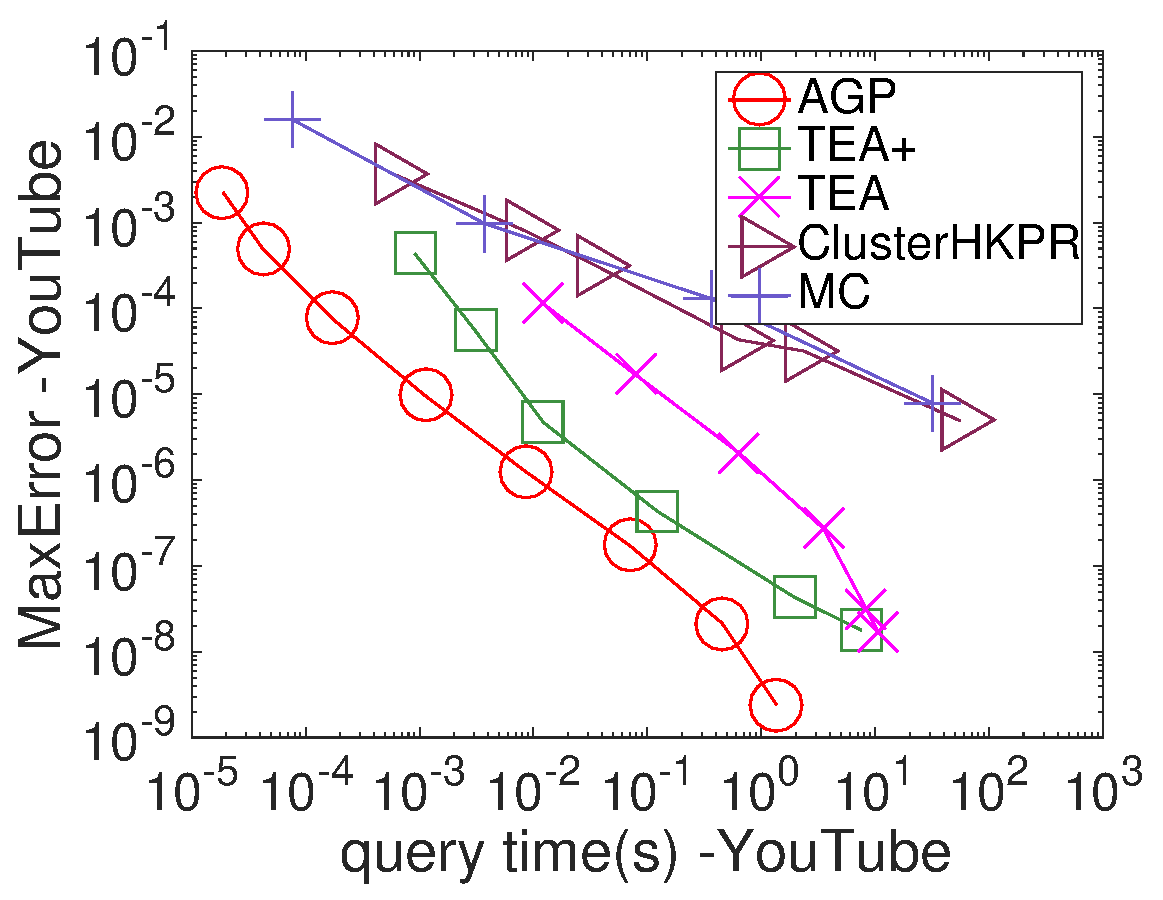
\includegraphics[height=34mm]{./Figs/HKPR-maxerr-query-YT.eps} &
			%\hspace{-3mm} 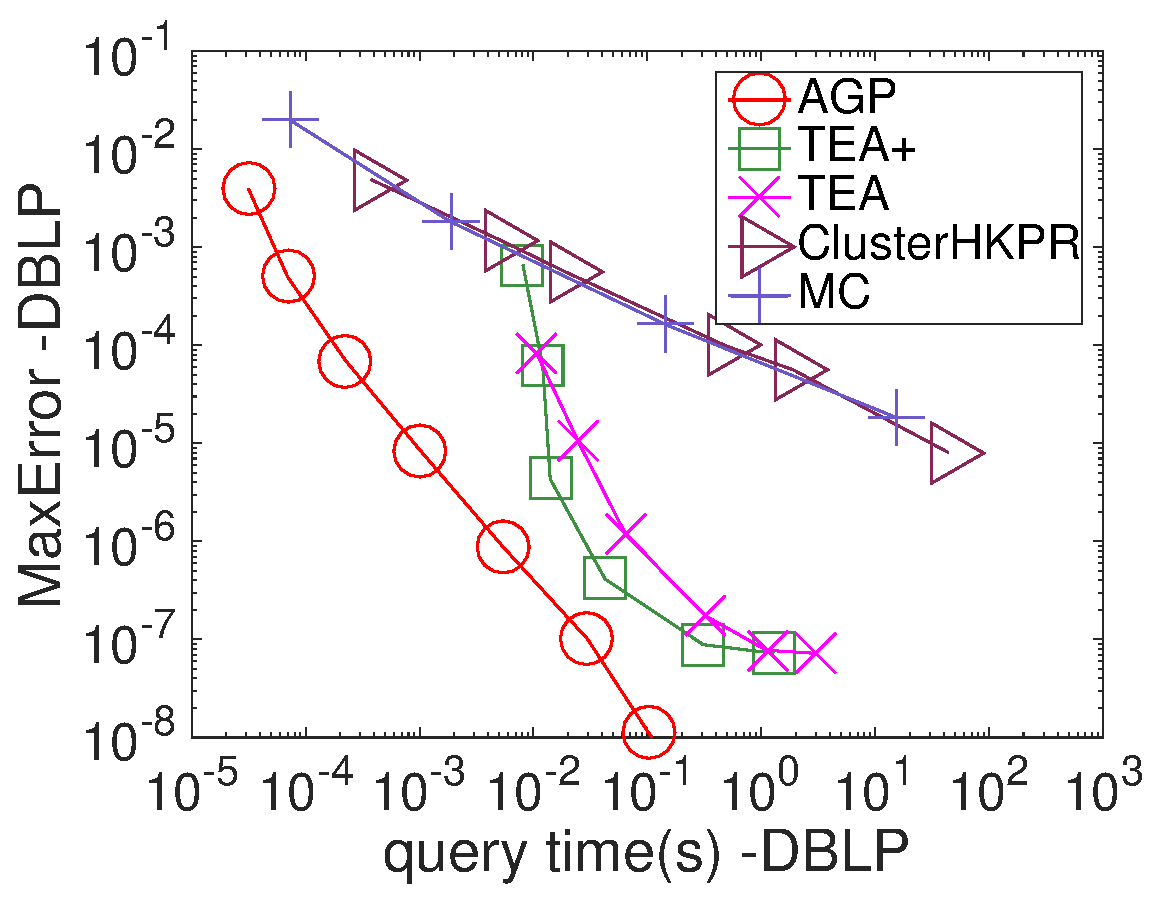
\includegraphics[height=25mm]{./Figs/HKPR-maxerr-query-DB.eps} &
			\hspace{-4mm} 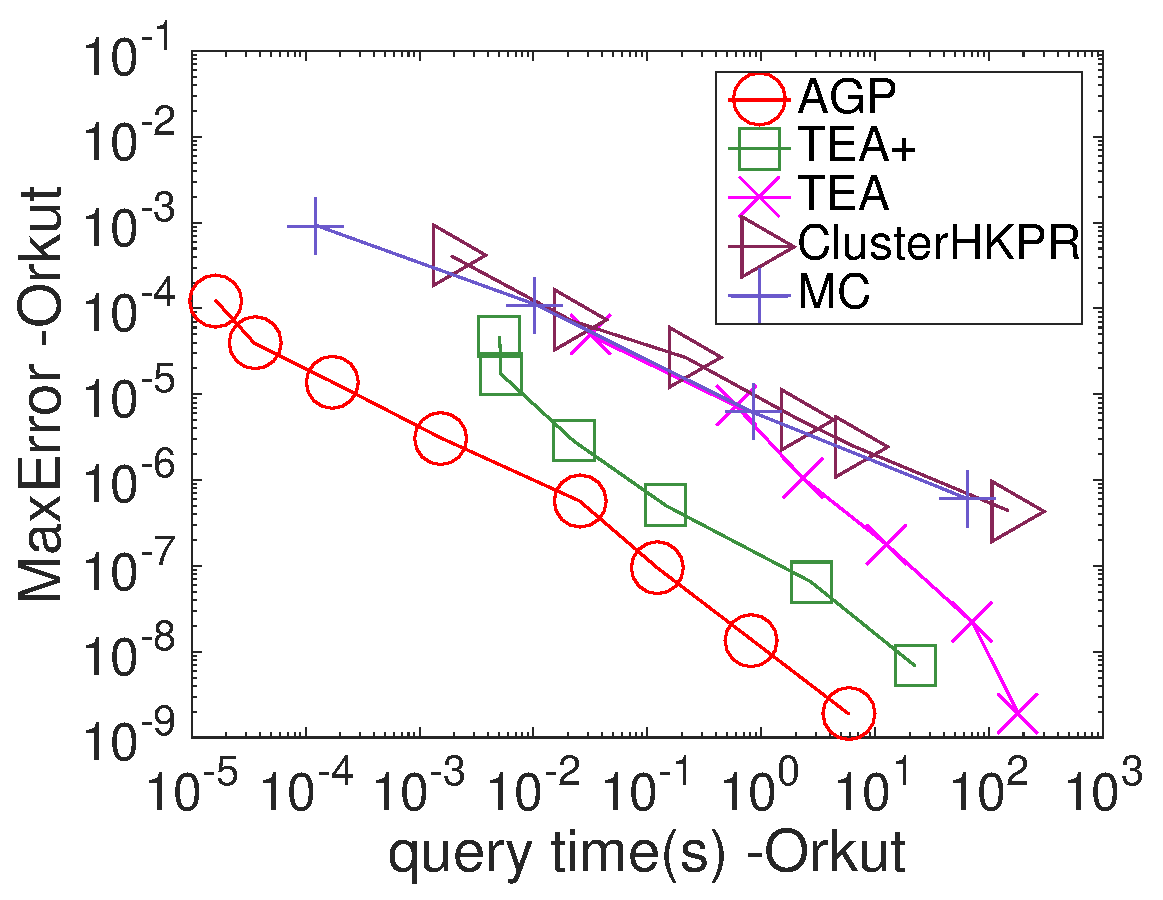
\includegraphics[height=34mm]{./Figs/HKPR-maxerr-query-OL.eps} &
			\hspace{-4mm} 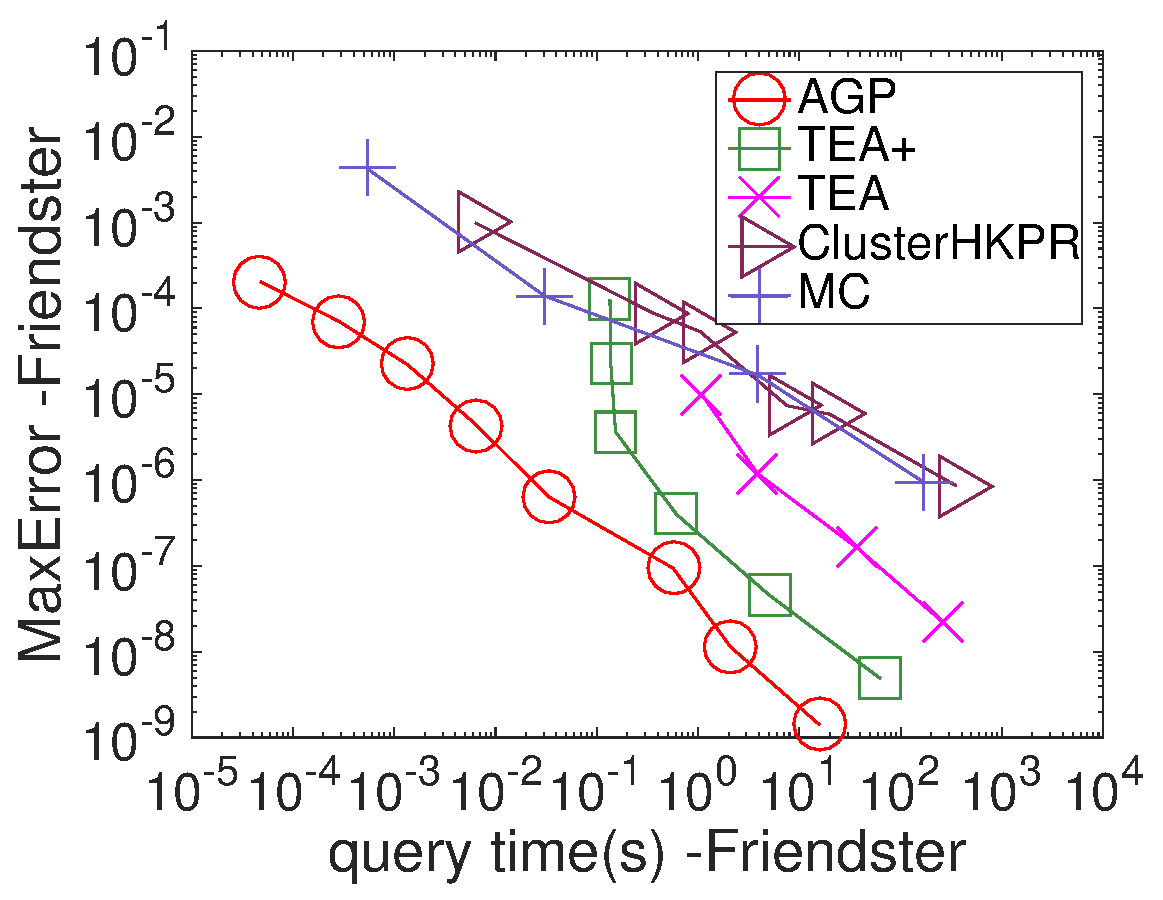
\includegraphics[height=34mm]{./Figs/HKPR-maxerr-query-FR.eps} &
			\hspace{-4mm} 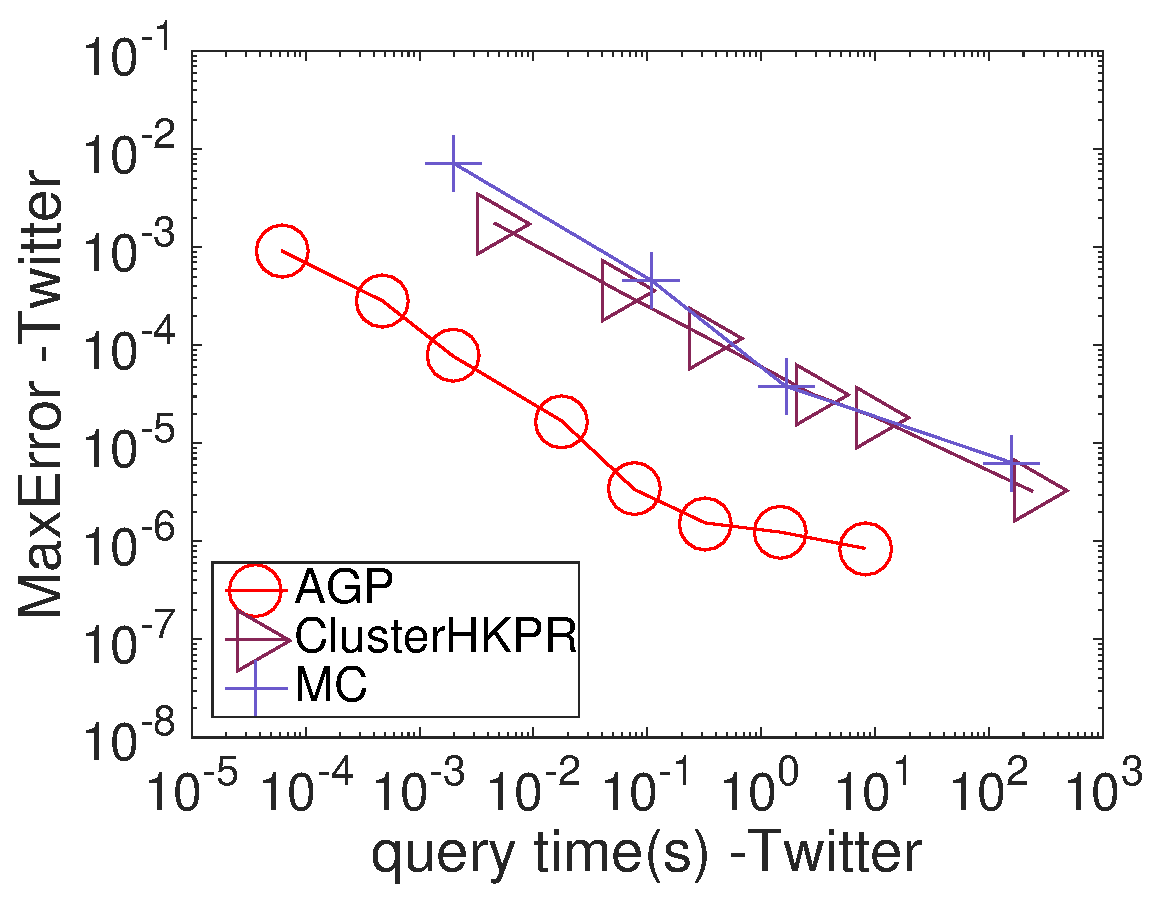
\includegraphics[height=34mm]{./Figs/HKPR-maxerr-query-TW.eps} 
		\end{tabular}
		\vspace{-5mm}
		\caption{Tradeoffs between {\em MaxError} and query time in local clustering.}
		\label{fig:HKPR-maxerror-query}
		\vspace{-2mm}
	\end{small}
\end{figure*}

\begin{figure}[t]
	\begin{small}
		\centering
		\vspace{-2mm}
		%    \begin{footnotesize}
		\begin{tabular}{cccc}
			%\multicolumn{4}{c}{\hspace{-4mm} \includegraphics[height=5mm]{./Figs/legend_large.eps}} \vspace{-1mm} \\
% 			\hspace{-2mm} 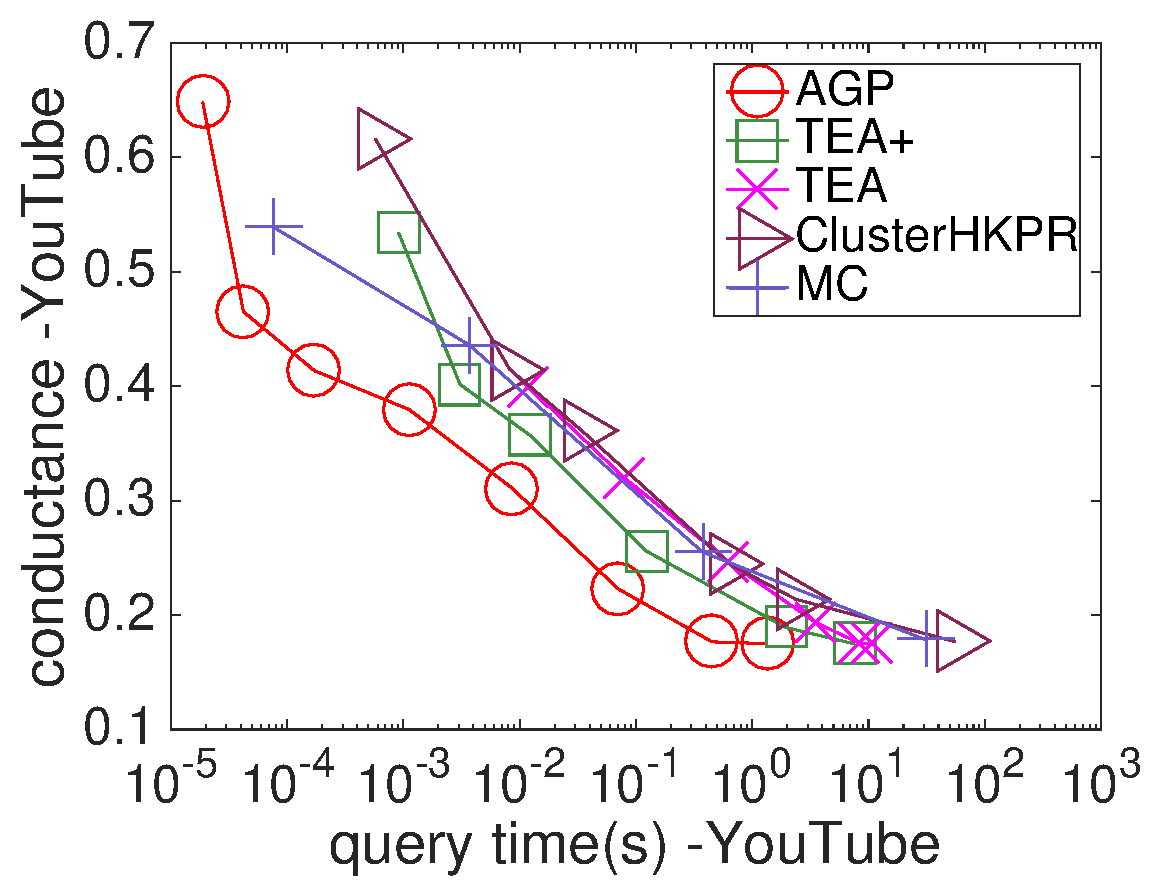
\includegraphics[height=34mm]{./Figs/HKPR-conductance-query-YT.eps} &
			%\hspace{-3mm} \includegraphics[height=25mm]{./Figs/HKPR-conductance-query-DB.eps} &
			\hspace{-4mm} 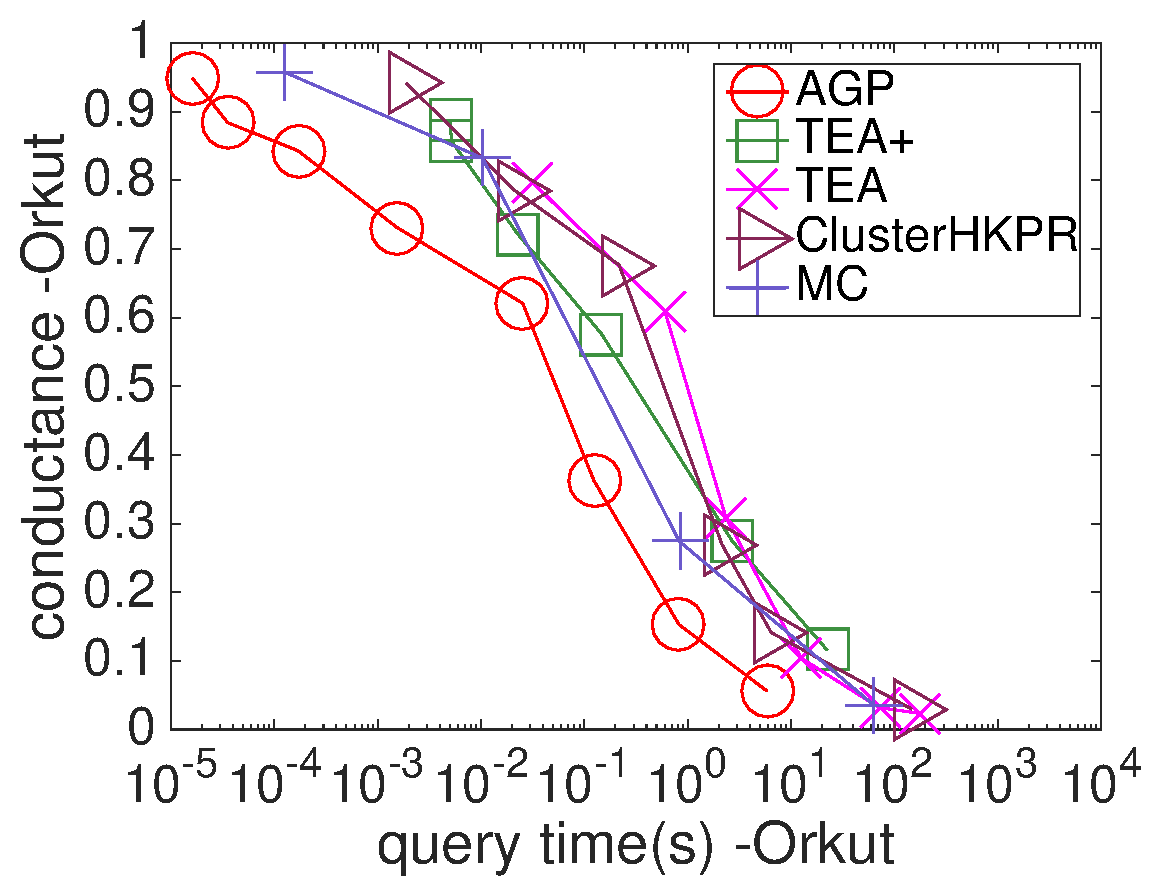
\includegraphics[height=32mm]{./Figs/HKPR-conductance-query-OL.eps} &
			\hspace{-4mm} 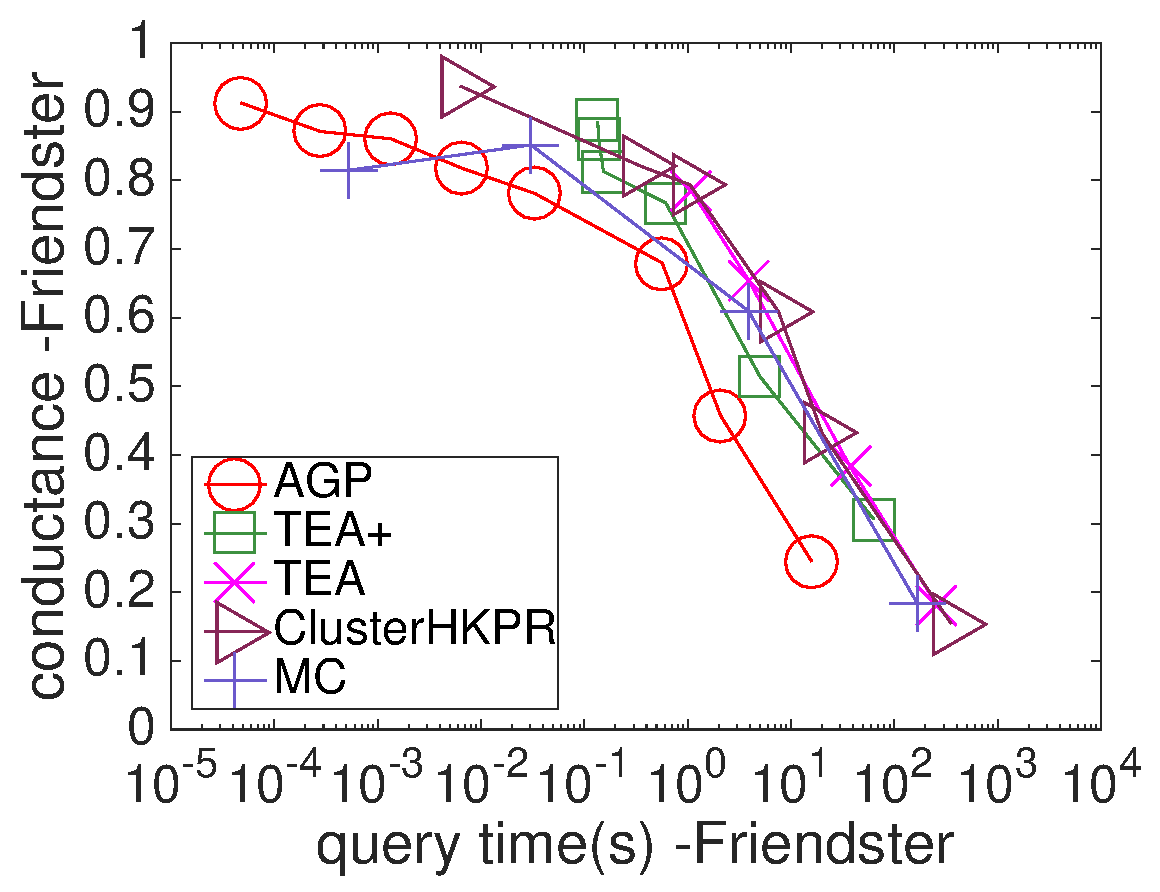
\includegraphics[height=32mm]{./Figs/HKPR-conductance-query-FR.eps} &
			%\hspace{-4mm} 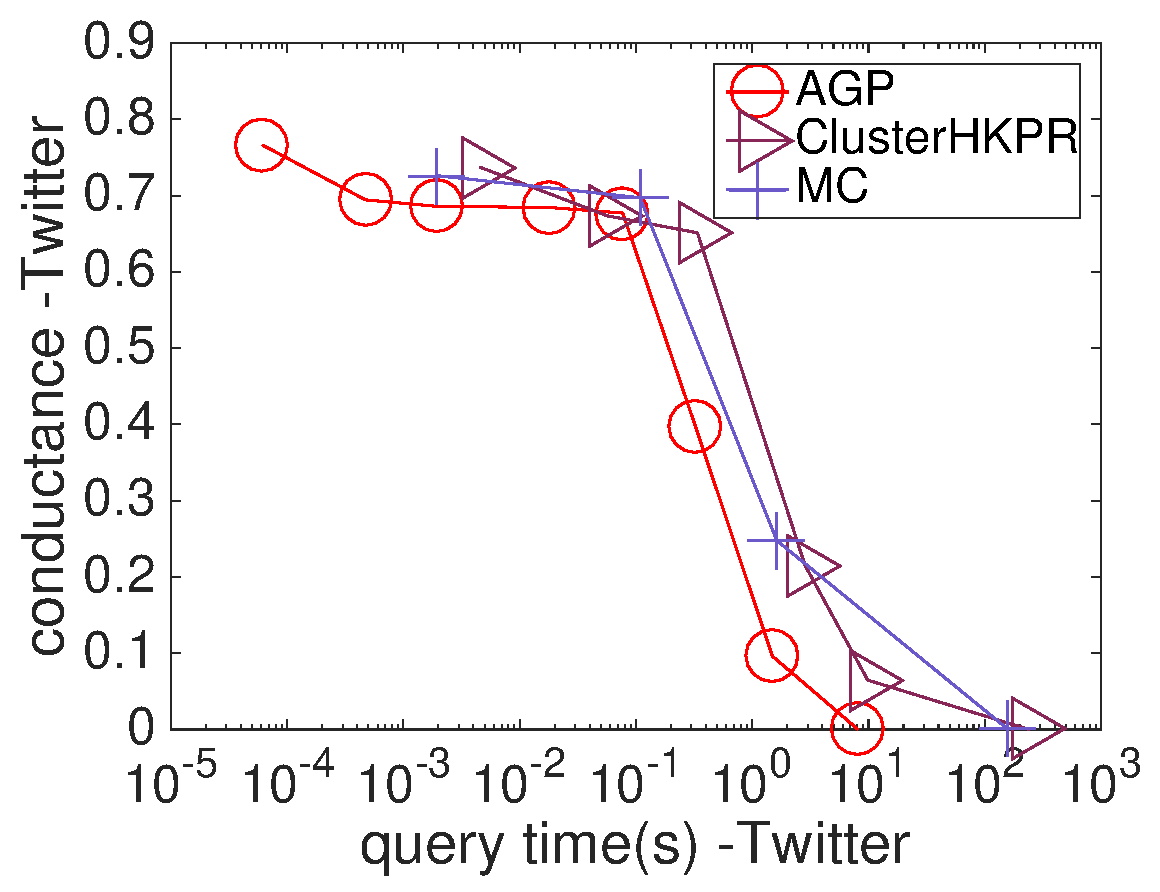
\includegraphics[height=34mm]{./Figs/HKPR-conductance-query-TW.eps} 
		\end{tabular}
		\vspace{-5mm}
		\caption{Tradeoffs between {\em conductance} and query time in local clustering.}
		\label{fig:HKPR-conductance-query}
		\vspace{-4mm}
	\end{small}
\end{figure}

In the next Lemma, we bound the variance of the approximate graph propagation vector $\hat{\pi}$, which takes a surprisingly simple form. 
\vspace{-1mm}
\begin{lemma}
\vspace{-1mm}
	\label{lem:variance}
    For any node $v \in V$, the variance of $\hat{\vec{\pi}}(v)$ obtained by Algorithm~\ref{alg:AGP-RQ} satisfies 
    %$	\Var \left[ \hat{\vec{\pi}}(v) \right]\le \frac{L(L+1)}{2} \cdot \varepsilon \cdot \vec{\pi}(v). $
    $	\Var \left[ \hat{\vec{\pi}}(v) \right]\le \frac{L(L+1)\varepsilon}{2} \cdot \vec{\pi}(v). $
    % \begin{equation}\nonumber
    % 	\begin{aligned}
    % 		\Var \left[ \hat{\vec{\pi}}(v) \right]\le \frac{L(L+1)}{2} \cdot \varepsilon \cdot \vec{\pi}(v). 
    % 	\end{aligned}
    % \end{equation}
\end{lemma}
\vspace{-1mm}
Recall that we can set $L=O(\log 1/\varepsilon)$ to obtain a relative error threshold of $\varepsilon$. Lemma~\ref{lem:variance} essentially states that the variance decreases linearly with the error parameter $\varepsilon$. Such property is desirable for bounding the relative error. In particular, for any node $v$ with $\vec{\pi}(v) > 100\cdot \frac{L(L+1)\varepsilon}{2}$, the standard deviation of $\hat{\vec{\pi}}(v)$ is bounded by ${1\over 10}\vec{\pi}(v)$. Therefore, we can set $\varepsilon = \delta \cdot \frac{200}{L(L+1)} = \Tilde{O}(\delta)$ and obtain the relative error guarantee in Definition~\ref{def:pro-relative}.
%implies that $\hat{\vec{\pi}}(v) - \vec{\pi}(v) \le  {1\over 10}\vec{\pi}(v)$ 
In particular, we have the following Theorem that bounds the expected cost of Algorithm~\ref{alg:AGP-RQ} under the relative error guarantee.

\vspace{-1mm}
\begin{theorem}\label{thm:RP-error}
Algorithm~\ref{alg:AGP-RQ} achieves an approximate propagation with relative error $\delta$, that is, for any node $v$ with $\vec{\pi}(v)>\delta$, $\left|\vec{\pi}(v)-\hat{\vec{\pi}}(v)\right|\hspace{-1mm} \leq \hspace{-1mm}\frac{1}{10} \cdot \vec{\pi}(v)$. The expected time cost can be bounded by
\vspace{-2mm}
\begin{equation*}
\vspace{-1mm}
E[Cost] =	O\left(\frac{L}{\delta}\cdot \sum_{i=1}^{L} \left\| Y_i \cdot \left(\mathbf{D}^{-a}\mathbf{A}\mathbf{D}^{-b} \right)^i \cdot \vec{x} \right\|_1\right).
\end{equation*}
\end{theorem}

To understand the time complexity in Theorem~\ref{thm:RP-error}, note that $ \left\| \left(\mathbf{D}^{-a}\mathbf{A}\mathbf{D}^{-b} \right)^i \cdot \vec{x} \right\|_1$ is the summation of the true residues at level $i$.  By the Pigeonhole principle, $ \frac{1}{\delta}\left\| Y_i \cdot \left(\mathbf{D}^{-a}\mathbf{A}\mathbf{D}^{-b} \right)^i \cdot \vec{x} \right\|_1$ is the upper bound of the residues at level $i$ that are larger than $\delta$. This bound is the output size of the propagation at level $i$, which means Algorithm~\ref{alg:AGP-RQ} achieves near optimal time complexity. 



Furthermore, we can compare the time complexity of Algorithm~\ref{alg:AGP-RQ} with other state-of-the-art algorithms in specific applications. For example, in the setting of heat kernel PageRank, the goal is to estimate $\vec{\pi}=\sum_{i=0}^\infty e^{-t} \cdot \frac{t^i}{i!}\cdot \left(\mathbf{A}\mathbf{D}^{-1} \right)^i \cdot \vec{e}_s $ for a given node $s$. The state-of-the-art algorithm TEA~\cite{yang2019TEA} computes an approximate HKPR vector $\hat{\vec{\pi}}$ such that for any $\pi(v)>\delta$, $|\vec{\pi}(v)-\hat{\vec{\pi}}(v)| \leq \frac{1}{10} \cdot \vec{\pi}(v)$ holds for high probability. By the fact that $t$ is the a constant and $\Tilde{O}$ is the Big-Oh notation ignoring log factors, the total cost of TEA is bounded by $O\left(t\log n \over \delta \right) = \Tilde{O}\left(1 \over \delta \right)$. On the other hand, in the setting of HKPR, the time complexity of Algorithm~\ref{alg:AGP-RQ} is bounded by 
\vspace{-2mm}
\begin{equation*}
\vspace{-2mm}
\frac{L}{\delta}\cdot \sum_{i=1}^{L} \left\| Y_i \cdot \left(\cdot \mathbf{A}^\top \mathbf{D}^{-1} \right)^i \cdot \vec{e}_s \right\|_1 = \frac{L}{\delta}\cdot \sum_{i=1}^{L} Y_i \le \frac{L^2}{\delta} = \Tilde{O}\left(1 \over \delta \right).
\end{equation*}
Here we use the facts that $ \left\| \left( \mathbf{A} \mathbf{D}^{-1} \right)^i \cdot \vec{e}_s \right\|_1 =1$ and $Y_i \le 1$. This implies that under the specific application of estimating HKPR, the time complexity of the more generalized  Algorithm~\ref{alg:AGP-RQ} is asymptotically the same as the complexity of TEA. Similar bounds also holds for Personalized PageRank and transition probabilities. We defer detailed explanation to the technical report~\cite{TechnicalReport}. 

	%For any $t \in V$ and $\ell \in \{0,1, 2, ... , L\}$, let $Z^{(\ell)}$ denote the term that:
%$$ Z^{(\ell)}(t)=\sum_{i=0}^{\ell-1} \frac{w_i}{Y_i}\hat{R}^{(i)}(t)+ \sum_{i=\ell}^{L}\sum_{u \in V} \frac{w_i}{Y_{\ell}} \cdot \hat{R}^{(\ell)}(u)\cdot p_{i-\ell}(u,t). $$
	 %The variance of $\hat{\pi}(t)$ obtained by Algorithm~\ref{alg:AGP-RQ} can be derived that:
    %\begin{align}\nonumber
    %	\Var \left[ \epi(t) \right]=\E \left[ \sum_{\ell=0}^{L-1}\Var \left[Z^{(\ell)}(t)\mid \hat{R}^{(0)},...,\hat{R}^{(\ell-1)}\right]\right]. 
    %\end{align}
		%Compute $p_{i+r_i} = \frac{1}{\delta}\cdot \frac{Y_{i+1}}{Y_i}\cdot \frac{\hat{\vec{r}}^{(i)}(u)}{d_{v_{i+r_i}}^a\cdot d_u^b}$ and add $v_{i+r_i}$ into $X$ with probability $\frac{p_{i+r_i}}{p_i}$\;\;
% consider the single-source PPR query from the source node $s$. Set $\delta=\frac{1}{n}$, which is commonly used in multiple applications. 
% $\vec{\hat{r}}^{(0)}(s)$ is initialized as $1$. $\vec{\hat{r}}^{(1)}(v_{1})=...=\vec{\hat{r}}^{(1)}(v_{n})=\frac{1-\alpha}{n}$ increased by the propagation from node $s$. Recall that the truncation rule asks to ignore all nodes with residues less than $\delta$. We need to abandon all propagations from node $v_{1},v_{1},...,$ and $v_{n}$ because $\vec{\hat{r}}^{(1)}(v_{j})=\frac{1-\alpha}{n}< \delta$ for $\forall j \in [1,n]$. Hence, $\hat{\vec{r}}^{(2)}(t)=0$ while the true value of residue $\vec{r}^{(2)}(t)=\left(1-\alpha\right)^2$. A large error can be caused by the simple truncation. 
%Simple truncation needs to be considered more efficiency. 
%So, truncate every nodes with small residues the trivial truncation leads to $\vec{\hat{r}}^{(2)}(t)=0$ and cause large error.  

% Indeed, consider the jump that start from neighbor $v_j$. The expectation of the geometric distributed random number $r$ is $1/p_j$, where $p_j$ is the probability of node $j$ being sampled. If $p_j$ is close to $0$, we may skip a large number of neighbors until the next sampled neighbor. 

% Actually, these is a sampling technique called {\em subset sampling} which can achieve independent sampling with small time cost. 
% We first illustrate the sampling process of subset sampling. Then we present the details to use subset sampling in our propagation structure. 
% %we conduct the sampling with the help of Sorted SubSet Sampling skill. 

% Considering an element set $S$, each element $x_i \in S$ has a pre-defined sampling probability $p_i$. The subset sampling problem wants to find an efficiency way to return the sample set, and guarantee each element $x_i \in S$ is sampled independently with the probability $p_i$. If we can pre-sort the elements $x_i \in S$ in the descending order of its sampling probability $p_i$, we call the problem as {\em sorted subset sampling}. 
% %To solve this problem, a naive method is to scan every element and check whether to be sampled one by one. We can guarantee independence of the sampling results by this naive way, while it's time cost is $O(|S|)$. If the sampling probability is relative small for the elements, $O(|S|)$ time cost can be much larger than the size of sampling results. 


% %As for the scenario that the sampling probability of each element is different, we can extend the above idea to further fix this problem. 

% Algorithm~\ref{alg:subsampling} extends the above idea for the scenario with different sampling probability. 
% %illustrates the pseudocode  to solve the Sorted SubSet Sampling problem. 
% Given the set $S$ of $h$ elements sorted by each element's sampling probability in the descending order, we initialize a variable $i$ as $0$, and a set $X$ as an empty set (Line 1). Then we repeat generating random numbers $r_i$ independently following the geometric distribution with parameter $p_i$ (Line 2-3). If $(i+r_i)$ does not exceed the number of elements $h$, we add the element $x_{i+r_i}$ to the set $X$ with probability $\frac{p_{i+r_i}}{p_i}$ (Line 4-6). Update $i$ as $(i+r_i)$ and move to the next iteration until $i$ exceeds $h$ (Line 7). After the process, we return the set $X$ as the sample set (Line 8). 
 
% %By theorem~\ref{thm:subsampling}, the Sorted Subset Sampling return the sample results efficiently and independently only if the sample elements sorted according to their sampling probability. 

% Note that the sorted subset sampling assumes all elements are sorted in the descending order of their sampling probability. In order to use sorted subset sampling in our propagation structure, we need to pre-sort the adjacency list of each node before the propagation process. Recall that for any node $u$ at level $i$, Algorithm~\ref{alg:AGP-RQ} samples the remained neighbors $v \in N_u$ with probability $p^{(i+1)}(u,v)=\frac{1}{\delta}\cdot \left(1-\frac{w_i}{Y_i} \right) \cdot \frac{\hat{R}^{(i)}(u)}{d_v^a\cdot d_u^b}$. Because the $d_u$ and $\hat{R}^{(i)}(u)$ are the same for every neighbor $v\in N_u$, we can sort the  adjacency list for $\forall v\in N_u$ only by $d_v$. The neighbors $\forall v\in N_u$ with large degrees correspond to small sampling probabilities.  
% % which is decreased by $d_v^a\cdot d_u^b$. Hence, we can pre-construct a sorted adjacency list for any node $u \in V$. 
% Thus we can append the neighbors $\forall v \in N_u$ to the adjacency list of $u$ by the ascending order of $d_v$. What's more, the sorting process can be finished in $O(m+n)$ time by counting sort, which asymptotically equals to the time cost of graph input. 

%Sorted Subset Sampling requires to sort every elements 


%As for the sampling process, a crucial point 
%In the sample process, if we check every neighbor to decide whether to sample, each propagation still cost $O(\bar{d})$, leading to the $O(m)$ cost for each iteration. 
%Hence, we adopt the techniques of subset sampling to finish the sample process during the time proportional to the size of the sampled set. 






%it asks to update the residue of all neighbors in every propagation operation, no matter how much the residue increases. 
%This costs $O(\bar{d})$ to touch every neighbor per propagation on average, where $\bar{d}$ denotes the average degree of the given graph. What's more, little residue can also increase the number of nodes with 





%\subsection{Subset Sampling}

 


%\subsection{Randomized Propagation}


% By this means, the number of nodes to be pushed in each iteration can be significantly  reduced. 
% Specifically, at each level $i\in [0,L-1]$, we pick the nodes $u$ to do the propagation only if $\hat{\vec{r}}^{(i)}(u)$ is larger than some threshold $\varepsilon$. By this means, the number of nodes to be pushed in each iteration can be significantly  reduced. 

%Moreover, note that in Algorithm~\ref{alg:AGP-deter}, the reserve $\hat{Q}^{(i)}(u)$ is only updated after the propagation from node $u$ at level $i$. If we decide not to do the propagation from node $u$
%Specifically, we can only pick the nodes $u$ satisfying $\left( 1- \frac{w_i}{Y_i}\right) \cdot \frac{\hat{R}^{(i)}(u)}{d_v^a\cdot d_u^b} \ge \delta$. Note that after the propagation from node $u$ at level $i$, for every neighbor $v\in N_u$, residue $\hat{R}^{(i+1)}(v)$ will be increased by $\left( 1- \frac{w_i}{Y_i}\right) \cdot \frac{\hat{R}^{(i)}(u)}{d_v^a\cdot d_u^b}$  according to the update rule. 

% To understand the variance bound of Algorithm~\ref{alg:AGP-RQ}, we observe that for each neighbor $v\in N_u$ with small degrees, we increase its residue by $\delta$ with probability $\frac{1}{\delta}\frac{Y_{i+1}}{Y_i} \cdot \frac{\hat{\vec{r}}^{(i)}(u)}{d_v^a\cdot d_u^b}$. Thus, the variance of this increment can be bounded by $ \delta^2\cdot \frac{1}{\delta}\frac{Y_{i+1}}{Y_i} \cdot \frac{\hat{\vec{r}}^{(i)}(u)}{d_v^a\cdot d_u^b} = \delta \cdot \frac{Y_{i+1}}{Y_i} \cdot \frac{\hat{\vec{r}}^{(i)}(u)}{d_v^a\cdot d_u^b} $. 

% for any node $u$ at level $i$, we transfer $\delta$ to its neighbors $v \in N_u$ with the probability $\frac{X^{(i+1)}(u,v)}{\delta}$. Thus, the variance of every propagation can be bounded by $\delta \cdot X^{(i+1)}(u,v)$. In each iteration from level $0$ to $L-1$,
% Meanwhile, the sum of residue increments totally received by nodes $v$ at level $i+1$ from its neighbors is $\vec{r}^{(i+1)}(v)=\sum_{u\in N_v} X^{(i+1)}(u,v)$. Hence, the variance of $\vec{r}^{(i+1)}(v)$ can be further bounded by $\delta \cdot \vec{r}^{(i+1)}(v)$. Sum up the variance of residues at the first $L$ levels. We can finally limit the variance of $\hat{\pi}(t)$ within $\delta \cdot \vec{\pi}(t)$ for every node $t \in V$, which is given in Lemma~\ref{lem:variance} in detail. 

% \begin{lemma}
% 	\label{lem:cost}
% 	The expected cost of Algorithm~\ref{alg:AGP-RQ} is bounded by
% 	\begin{align*}
% 	\E \left[Cost\right] \leq \frac{1}{\delta}\cdot \sum_{i=1}^{L} \left\| Y_i \cdot \left(\mathbf{D}^{-a}\cdot \mathbf{A}^\top \cdot \mathbf{D}^{-b} \right)^i \cdot \vec{x} \right\|_1.
% 	%\E \left[C_{total}\right] \leq \sum_{i=0}^{L-1} \sum_{v\in V} \frac{1}{\delta}\cdot R^{(i+1)}(v).
% 	\end{align*}
% \end{lemma}
% As for the total cost of Algorithm~\ref{alg:AGP-RQ}, we first consider the cost of one propagation, and sum them up in the end. For the propagation from node $u$ at level $i$ to its neighbor $v$, it will cost $1$ deterministically if $X^{(i+1)}(u,v)< \delta$, or with the probability $\frac{X^{(i+1)}(u,v)}{\delta}$ otherwise. Hence, the cost of one propagation can also be bounded by $\frac{X^{(i+1)}(u,v)}{\delta}$. Sum up all propagation for any node at the first levels. The total cost can be bounded by $\sum_{i=0}^{L-1}\sum_{v\in N_u} \frac{X^{(i+1)}(u,v)}{\delta}=\sum_{i=0}^{L-1} \frac{\vec{r}^{(i+1)}(v)}{\delta}$, which approximately equals the number of residues more than $\delta$ in the first levels. Recall that in Definition~\ref{def:pro-relative}, we want to estimate $\pi(t)$ precisely if $\pi(t)\ge \delta$. Thus, the number of residues more than $\delta$ is actually a lower bound of the propagation structure, and the cost of Algorithm~\ref{alg:AGP-RQ} achieves optimal asymptotically. 




% Finally, based on the three Lemma given above, we can derive Theorem~\ref{thm:RP-error}, which gives the error bound and time cost of our randomized propagation structure. 
%The proof of Theorem~\ref{thm:RP-error} can be divided into several parts given by the lemmas below. Lemma~\ref{lem:unbiasedness} first shows the unbiasedness of $\epi$. While Lemma~\ref{lem:variance} and Lemma~\ref{lem:cost} bound the variance and cost of $\epi$ derived by Algorithm~\ref{alg:AGP-RQ}. 




% \noindent{\bf Remarks.}



% we set the maximum level to do the propagation $L=\log{\frac{1}{\delta}}$ according to Assumption~\ref{asm:L} (Line 1). For each $i \in [0,L]$, initialize all vectors of $i$-hop residues and reserves as $\vec{0}$, except $\vec{\hat{r}}^{(0)}=\vec{x}$ (Line 2-3). In the iteration from level $0$ to $L-1$, we only deterministically do the propagation from the nodes $u$ to its neighbors $v\in N_u$, which satisfy $d_v^a\cdot d_u^b \hspace{-0.5mm} \le \hspace{-0.5mm} \frac{\hat{\vec{r}}^{(i)}(u)}{\delta} \cdot \frac{Y_{i+1}}{Y_i}$. 
% %In the propagation from node $u$ at level $i$ to its neighbor $v\in N_u$, 
% %For these node $u$ and their corresponding neighbors $v\in N_u$, 
% And increase $\hat{\vec{r}}^{(i+1)}(v)$ by $\frac{Y_{i+1}}{Y_i}\cdot \frac{\hat{\vec{r}}^{(i)}(u)}{d_v^a\cdot d_u^b}$ (Line 6-7). For the other neighbors $v \in N_u$, we sample them with the probability $\frac{1}{\delta}\cdot \frac{Y_{i+1}}{Y_i} \cdot \frac{\hat{\vec{r}}^{(i)}(u)}{d_v^a\cdot d_u^b}$ (Line 8-9). Then we transfer $\frac{w_i}{Y_i}\cdot \hat{\vec{r}}^{(i)}(u)$ to the reserve $\hat{\vec{q}}^{(i)}(u)$ and set $\hat{\vec{r}}^{(i)}(u)$ as $0$ (Line 10-11). After the $L_{th}$ iteration, return $\sum_{i=0}^L \hat{\vec{q}}^{(i)}$ as the estimation of $\pi$ (Line 12). 





% Again, we consider the toy graph in Figure~\ref{fig:special-case} and the task of estimating the 2-step transtion probability vector $\pi=\left(\mathbf{A} \cdot \mathbf{D}^{-1} \right)^2 \cdot \vec{e}_s $ from node $s$. As previously stated, to perform the propagation from $s$, we need to sample a small subset from $s$' neighbor set $N(s) = \{v_1, \ldots, v_n\}$.

% Even though each propagation received by node $t$ only brings quite small increments to its residue, a large number of propagations can accumulate these increments to a large residue.  


% Hence, other than truncate every propagation from the nodes with small residues, it's better to sample some neighbors to do the propagations. In detail, for each node $u \in V$ at level $i$ ($i\in [0,L-1]$), let $X^{(i+1)}(u,v)$ denote the residue increment of $\hat{\vec{r}}^{(i+1)}(v)$ caused by the propagation from node $u$ to its neighbor $v\in N_u$. 
% %For those propagations to some neighbors $v$ with small residue increment, such that 
% If $X^{(i+1)}(u,v)< \delta$, we can sample node $v$ with the probability $\frac{X^{(i+1)}(u,v)}{\delta}$ to determine whether propagating from node $u$ to $v$. Small residue increments correspond to small sampling probabilities. The sampling process only focus on the propagation with small residue increments. Thus, only a few number of sampling is expected to be conducted.  
% Thus, by this means, we can effectively avoid the error caused by the simple truncation without obviously extra time cost.
% %We can sample the neighbors to conduct the propagations 
% %it's better to truncate the propagation with small residue increments wisely, other than focus on nodes with small residues.
% %as for these propagation with little residue increments, we can use sampling to decide which to propagate, other than truncating these nodes trivially. 
% %Randomness can avoid the simple propagation truncation. 

% %Based on this idea, we propose a Randomized Propagation Algorithm, using randomness to avoid the large error caused by the truncated propagation. 


% Recall that we denote $X^{(i+1)}(u,v)$ as the increment of residue $\hat{\vec{r}}^{(i+1)}(v)$ caused by the propagation from node $u$ to $v$ ($v\in N_u$). By the recursive formula given in equation~\eqref{eqn:iteration}, $X^{(i+1)}(u,v)$ is expected to be $\frac{Y_{i+1}}{Y_i} \cdot \frac{\hat{\vec{r}}^{(i)}(u)}{d_v^a\cdot d_u^b}$. Algorithm~\ref{alg:AGP-RQ} deterministically do the propagation when this increment $X^{(i+1)}(u,v)$ is more than $\delta$, and use sampling to reduce the number of propagation with unbiasedness. 
%Note that in the propagation from node $u$ at level $i$ to its neighbor $\forall v\in N_u$, residue $\hat{R}^{(i+1)}(v)$ is expected to be increased by $\frac{Y_{i+1}}{Y_i} \cdot \frac{\hat{R}^{(i)}(u)}{d_v^a\cdot d_u^b}$  according to the update rule given in equation~\eqref{eqn:iteration}. 



% For ease of presentation, we first consider the simple case where $d_{v_1} = d_{v_2} = \ldots = d_{v_{d_v}}$. It follows that $p_1 = p_2= \ldots = p_{d_v}$. 


% If the sampling probability is identical for every element, denoting as $p$, we can generate a binomial random number $r\sim B(|S|,p)$ first. %$r$ tells us the number of elements to be sampled. 
% Then we generate $r$ uniform random numbers corresponding to the element ID to be sampled. In this way, we can finish the sampling process within the time $1+h$, where $h=|S|$. % denotes the number of elements in the element set $S$. 
% Moreover, we can further polish the sampling process by substituting geometric random number for the binomial random number. Denote a geometric random number $r_g\sim G(p)$, which means we need to go through $r_g-1$ failure before the first success. 
% Instead of using binomial random number to decide the number of sampling, it's better to repeat generating geometric random numbers to find the next element successfully sampled. We can save no less than 1 cost than to generate binomial random numbers. 



% for any node $u\in V$ at level $i$ ($i \in [0,L-1]$), we want to sample from those neighbors $v\in N_u$ to which whether propagating, when the residue increment $X^{(i+1)}(u,v)<\delta$. But if we check these candidate neighbors one by one, the time cost is equivalent to the power method actually. 
% %During the sample process, we aim to return the sample results with the time proportional to the size of the sample set. So we cannot scan every neighbor and decide whether to sample one by one. Otherwise, each propagation still cost $O(\bar{d})$, which is also a global propagation process and don't save time.
% % Wang et al.~\cite{wang2020RBS} propose a sampling technique to generate one random number for all neighbors. %They use the identical random number to sample every neighbor to be propagated. 
% %Though they can achieve a fast sampling with the time cost equals to the size of the sample set, every sampling is dependent for $\forall v\in N_u$. 
% How can we sample neighbors independently with the time cost proportional to the sample set? 

%With the help of sorted subset sampling, we can choose the neighbors independently without check every nodes meanwhile.

%%% Local Variables:
%%% mode: latex
%%% TeX-master: "paper"
%%% End:

%\section{Optimization}
\vspace{+1mm}

%\hspace*{\fill} \\
%\hspace*{\fill} \\
\vspace{+1mm}
%\subsection{Edge-based $\ell$-hop Backward Push} \label{sec:edgebased_lhoppush}





%\subsection{$\sqrt{1-\alpha}$-walk} \label{sec:alpha_walk}





%%% Local Variables:
%%% mode: latex
%%% TeX-master: "paper"
%%% End:

\header{\bf Propagation on directed graph.}
Our generalized propagation structure can also extend to directed graph by $\pi=\sum_{i=0}^\infty w_i \cdot \left(\D^{-a}\tilde{\A}\D^{-b} \right)^i \cdot \vec{x},$
% \begin{equation}\label{eqn:pi_gen_directed}
% \vspace{-2mm}
% 	\begin{aligned}
% 		\pi=\sum_{i=0}^\infty w_i \cdot \left(\bm{D}^{-a}\cdot \tilde{\bm{A}} \cdot \bm{D}^{-b} \right)^i \cdot \vec{x}, 
% 	\end{aligned}
% \end{equation}
where $\bm{D}$ denotes the diagonal out-degree matrix, and $\tilde{\A}$ represents the adjacency matrix or its transition according to specific applications. For PageRank, single-source PPR, HKPR, Katz we set $\tilde{\A}=\A^\top$ with the following recursive equation: 
\vspace{-2mm}
\begin{equation}\nonumber
\vspace{-2mm}
	\begin{aligned}
		\vec{r}^{(i+1)}(v)=\sum_{u\in N_{in}(v)} \left(\frac{Y_{i+1}}{Y_i} \right) \cdot \frac{\vec{r}^{(i)}(u)}{d_{out}^{a}(v) \cdot d_{out}^b(u)}. 
	\end{aligned}
\end{equation}
where $N_{in}(v)$ denotes the in-neighbor set of node $v$ and $d_{out}(u)$ is the out-degree of node $u$. 
% In comparison, for the propagation structure starting from a given target node, such as single-target PPR query,  $\tilde{\bm{A}}$ is set as $\bm{A}$ and 
% \begin{equation}\nonumber
% \vspace{-2mm}
% 	\begin{aligned}
% 		\vec{r}^{(i+1)}(v)=\sum_{u\in N_{out}(v)} \left(\frac{Y_{i+1}}{Y_i} \right) \cdot \frac{\vec{r}^{(i)}(u)}{d_{out}^{a}(v) \cdot d_{out}^b(u)}, 
% 	\end{aligned}
% \end{equation}
% where in each iteration, we update the residues of in-neighbors. 
% Beyond that, the propagation process and the complexity analysis are the same with that on undirected graphs. 







%In detail, as for PageRank and single-source PPR query, the propagation equation is that
%\begin{equation}\nonumber
%	\begin{aligned}
%		\pi=\sum_{i=0}^\infty \alpha \left( 1-\alpha \right)^i \cdot \left(\mathbf{A}^\top \mathbf{D}^{-1} \right)^i \cdot \vec{x}, 
%	\end{aligned}
%\end{equation}
%where $\vec{x}=\left(\frac{1}{n}\cdot \vec{1}\right)$ for PageRank, and $\vec{x}=\vec{e}_s$ for single-source PPR query. 
%The propagation structure of HKPR is similar with single-source PPR, except $w_i=\frac{e^{-t}t^i}{i!}$ following the poisson distribution with constant $t$ as parameter. Katz set $\tilde{\mathbf{A}}=A^\top$

%For example, as for PageRank, single-source PPR query, Katz, HITS, HKPR and so on, $\tilde{\bm{A}}$ should be set as $\bm{A}^\top$ that each propagation update the residue and reserve of out-neighbors. 





%where $\tilde{N}(v)=N_{in}(v)$ if $\mathbf{\tilde{A}}=\mathbf{A}^\top$ in the generalized equation~\eqref{eqn:pi_gen}, or $\tilde{N}(v)=N_{out}(v)$ if $\mathbf{\tilde{A}}=\mathbf{A}$. 


%If the $\tilde{A}=A^\top$ in the propagation structure, such as the single-source PPR query, HITS, Katz, and HKPR, we add $\hat{R}^{(i+1)}(v)$ by $\left(1-\frac{w_i}{Y_i} \right) \cdot \frac{\hat{R}^{(i)}(u)}{d_v^{1-r} \cdot d^r_u}$ for every out-neighbors $v\in N_o(u)$ (Line 6-7). While if $\tilde{A}=A$ such as the single-target PPR query, we update the residue for every in-neighbor of node $u$. 


\begin{comment}
\begin{table*}[t]
	%\vspace{-2mm}
	\centering
	\renewcommand{\arraystretch}{1.5}
	\tblcapup
	\caption{Typical propagation equations.}
	\vspace{-3mm}
	\tblcapdown
%	\begin{small}
		\begin{tabular}{|c|c|c|c|c|c|c|c|} \hline
			\multicolumn{2}{|c|}{\bf Algorithm} & {\bf $\boldsymbol{\tilde{A}}$}& {\bf $\boldsymbol{a}$}& {\bf $\boldsymbol{b}$} & {\bf $\boldsymbol{w_i}$} & {\bf $\boldsymbol{\vec{x}}$} & {\bf Propagation equation} \\ \hline
			\multicolumn{2}{|c|}{PageRank} & $\mathbf{A}^\top$ & $a=0$ & $b=1$& $\alpha \left( 1-\alpha \right)^i $ & $\frac{1}{n}\cdot \vec{1}$ & $\pi=\sum_{i=0}^\infty \alpha \left( 1-\alpha \right)^i \cdot \left(\mathbf{A}^\top \cdot \mathbf{D}^{-1} \right)^i \cdot \left(\frac{1}{n}\cdot \vec{1} \right)$ \\ \hline
			\multicolumn{2}{|c|}{single-source PPR} &$\mathbf{A}^\top$ &$a=0$ & $b=1$ & $\alpha \left( 1-\alpha \right)^i $ & one-hot vector $\vec{e}_s$ & $\pi=\sum_{i=0}^\infty \alpha \left( 1-\alpha \right)^i \cdot \left(\mathbf{A}^\top  \cdot \mathbf{D}^{-1} \right)^i \cdot \vec{e}_s $ \\ \hline
			\multicolumn{2}{|c|}{single-target PPR} &$\mathbf{A}$ & $a=1$ & $b=0$ & $\alpha \left( 1-\alpha \right)^i $ & one-hot vector $\vec{e}_t$ & $\pi=\sum_{i=0}^\infty \alpha \left( 1-\alpha \right)^i \cdot \left(\mathbf{D}^{-1} \cdot \mathbf{A} \right)^i \cdot \vec{e}_t $\\ \hline
			\multicolumn{2}{|c|}{HKPR} &$\mathbf{A}^\top$ &$a=0$ & $b=1$ & $e^{-t} \cdot \frac{t^i}{i!} $ & one-hot vector $\vec{e}_s$ & $\pi=\sum_{i=0}^\infty e^{-t} \cdot \frac{t^i}{i!}\cdot \left(\mathbf{A}^\top  \cdot \mathbf{D}^{-1} \right)^i \cdot \vec{e}_s $\\ \hline
			%\multicolumn{2}{|c|}{$k$-hop transition probability} & $r=1$ & $w_i=0 (i \neq k), w_k=1$ & one-hot vector $\vec{e}_s$ & $\left(\mathbf{A} \cdot \mathbf{D}^{-1} \right)^k \cdot \vec{e}_s $\\ \hline
			\multirow{3}{*}{GNN} & SGC,GCN &$\mathbf{A}^\top$ & $a=\frac{1}{2}$ & $b=\frac{1}{2}$ & $w_i=0 (i \neq k), w_k=1$ & feature vector $\vec{x}$ & $\pi=\left(\mathbf{D}^{-\frac{1}{2}} \cdot \mathbf{A} \cdot \mathbf{D}^{-\frac{1}{2}} \right)^k \cdot \vec{x} $\\ \cline{2-8}
			~& APPNP &$\mathbf{A}^\top$ &  $a=\frac{1}{2}$ & $b=\frac{1}{2}$ & $\alpha \left( 1-\alpha \right)^i$ & feature vector $\vec{x}$ & $\pi=\sum_{i=0}^k \alpha \left( 1-\alpha \right)^i \cdot \left(\mathbf{D}^{-\frac{1}{2}} \cdot \mathbf{A} \cdot \mathbf{D}^{-\frac{1}{2}} \right)^i \cdot \vec{x} $ \\ \cline{2-8}
			~& GDC &$\mathbf{A}^\top$ &  $a=\frac{1}{2}$ & $b=\frac{1}{2}$ & $e^{-t} \cdot \frac{t^i}{i!} $  & feature vector $\vec{x}$ & $\pi=\sum_{i=0}^k e^{-t} \cdot \frac{t^i}{i!}\cdot \left(\mathbf{D}^{-\frac{1}{2}} \cdot \mathbf{A} \cdot \mathbf{D}^{-\frac{1}{2}} \right)^i \cdot \vec{x} $ \\ \hline
			\multicolumn{2}{|c|}{Katz} &$\mathbf{A}^\top$ & $a=0$ & $b=0$ & $\beta^i$ & one-hot vector $\vec{e}_s$ & $\pi=\sum_{i=0}^\infty \beta^i \cdot \left(\mathbf{A}^\top \right)^i \cdot \vec{x}$\\ \hline
			\multicolumn{2}{|c|}{HITS} &$\mathbf{A}^\top$ & $a=0$ & $b=0$ & $w_i=\frac{1}{\mu_{j}}(i=2j)$, or $w_i=0$ & $\frac{1}{n}\cdot \vec{1}$ & $\pi=\sum_{j=0}^\infty \frac{1}{\mu_j}\cdot \left(\mathbf{A}^\top\right)^{2j} \cdot \vec{1}$ \\ \hline	
		\end{tabular}
%	\end{small}
	%\label{tbl:propagation}
	%\tbldown
	%\vspace{-3mm}
\end{table*}

\end{comment}



%%% Local Variables:
%%% mode: latex
%%% TeX-master: "paper"
%%% End:

%
\section{Applications} \label{sec:applications}

detailed description

\header{\bf Propagation in node proximity.} 
\begin{itemize}
	\item PageRank
	\item PPR
	\item HKPR
\end{itemize}
 

\header{\bf Propagation in GNN.} 
\begin{itemize}
	\item SGC
	\item GCN
	\item APPNP
	\item GDC
\end{itemize}



%%% Local Variables:
%%% mode: latex
%%% TeX-master: "paper"
%%% End:

\vspace{-1mm}
\section{Experiments} \label{sec:exp}

\begin{table}[t]
	\vspace{-2mm}
	\centering
	\tblcapup
	\caption{Datasets for local clustering.}
	\vspace{-4mm}
	\tblcapdown
	\begin{small}
		\begin{tabular}{|l|l|r|r|} %p{1.3in}|}
			\hline
			{\bf Data Set} & {\bf Type} & {\bf $\boldsymbol{n}$} & {\bf $\boldsymbol{m}$}	 \\ \hline
			%ca-GrQc (GQ) & undirected & 5,242 & 28,968\\
			%AS-2000(AS) & undirected & 6,474 & 25,144\\
			%CA-HepTh(HT) & undirected & 9,877 & 51,946\\
			%Wikivote (WV) & directed & 7,115 & 103,689\\
			%CA-HepPh (HP) & undirected & 12008 & 236978\\
			% Wiki-Vote(WV)	& 	directed &	7,155	&	103,689 \\
			% {HepTh(HT)}	    & 	undirected &	9,877	&	25,998		\\
			% {AS-Caida(AC)}	    &	directed &	26,475	&	106,762		\\
			% {HepPh(HP)}	        &	directed &	34,546	&	421,578 \\
			% Cnr-2000 (CN) & directed & 325,557 &	3,216,152 \\
			% {Web-Google(WG)} & directed & 875,713 &	5,105,039 \\)
			%As-Skitter (AS) & undirected & 1,696,415	& 11,095,298 \\
			%      {\color{red} In-2004(IN) } & directed & 1,382,908	& 16,917,053
			% \\
			YouTube  & undirected & 1,138,499 & 5,980,886 \\
			%DBLP-Author  & undirected & 5,425,963 & 17,298,032 \\
			% {Com-LiveJournal(CL)} & undirected & 3,997,962	& 34,681,189 \\
			%LiveJournal (LJ) &	directed & 4,847,571 & 68,475,391\\
			%IndoChina (IC)	& 	directed &	7,414,768  &	191,606,827		\\
			Orkut-Links  & undirected & 3,072,441 & 234,369,798 \\		
			%DBpediaLink (DL) & directed & 18,268,992 & 172,183,984 \\
			%WikiLink(WL) & directed & 12,150,976 & 378,142,420 \\
			% { Web-Base}   & { directed} & {
			% 118,142,155} & { 1,019,903,190} \\
			%Web-Base (WB) & directed & 118,142,155& 1,019,903,190 \\
			%It-2004 (IT)	&	directed & 41,290,682 & 1,135,718,909\\	
			Twitter  & directed & 41,652,230& 1,468,364,884 \\
			%SK-2005 (SK) & directed & 50,636,154	& 1,949,412,601 \\
			Friendster   & undirected & 68,349,466 & 3,623,698,684 \\
			%UK-Union (UK) & directed & 133,633,040 & 5,507,679,822 \\
			\hline
		\end{tabular}
	\end{small}
	\label{tbl:datasets}
	%\tbldown
	\vspace{-5mm}
\end{table}

This section experimentally evaluates AGP's performance in two concrete applications: local clustering with heat kernel PageRank and node classification with GNN. Specifically, Section~\ref{subsec:clustering} presents the experimental results of AGP in local clustering. Section~\ref{subsec:GNN} evaluates the  effectiveness of AGP on existing GNN models. 


% \begin{figure*}[!t]
% 	\begin{small}
% 		\centering
% 		\vspace{-1mm}
% 		%    \begin{footnotesize}
% 		\begin{tabular}{cccc}
% 			%\multicolumn{4}{c}{\hspace{-4mm} \includegraphics[height=5mm]{./Figs/legend_large.eps}} \vspace{-1mm} \\
% 			\hspace{-2mm} 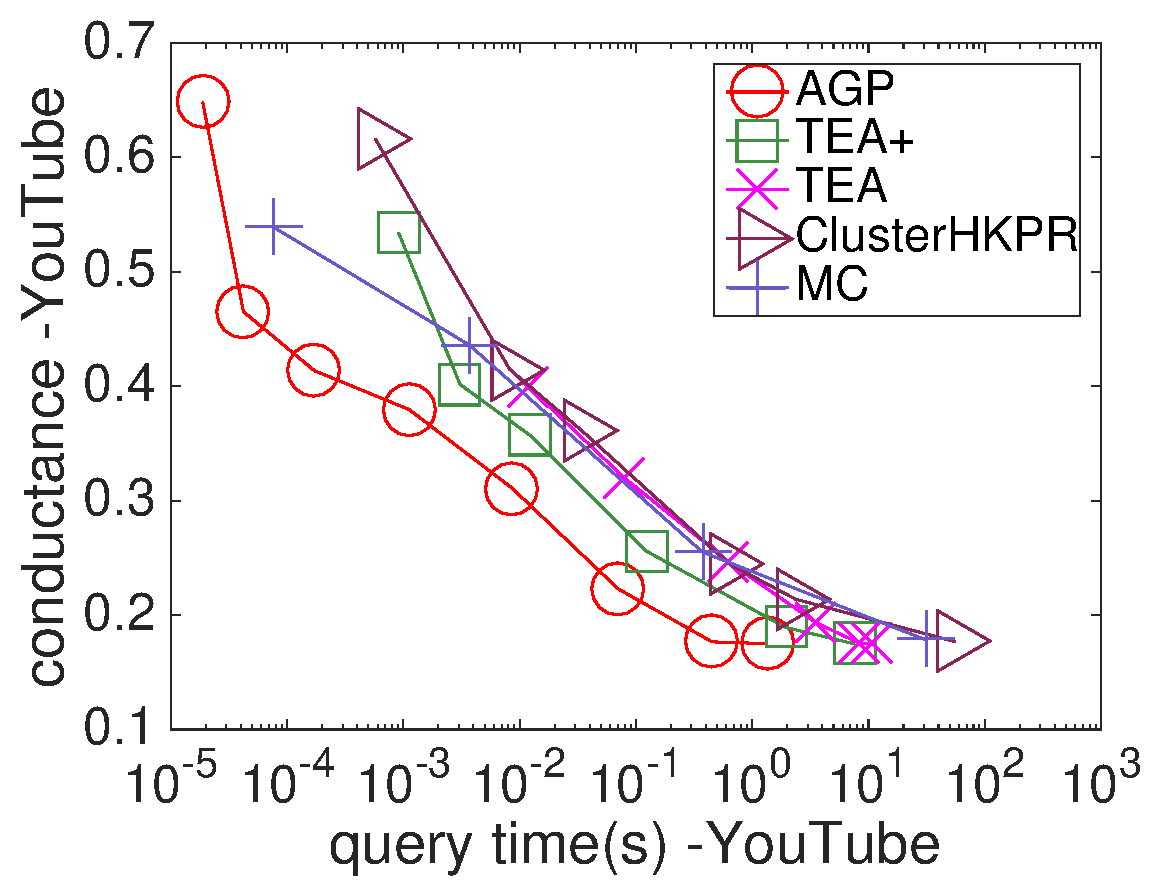
\includegraphics[height=34mm]{./Figs/HKPR-conductance-query-YT.eps} &
% 			%\hspace{-3mm} \includegraphics[height=25mm]{./Figs/HKPR-conductance-query-DB.eps} &
% 			\hspace{-4mm} 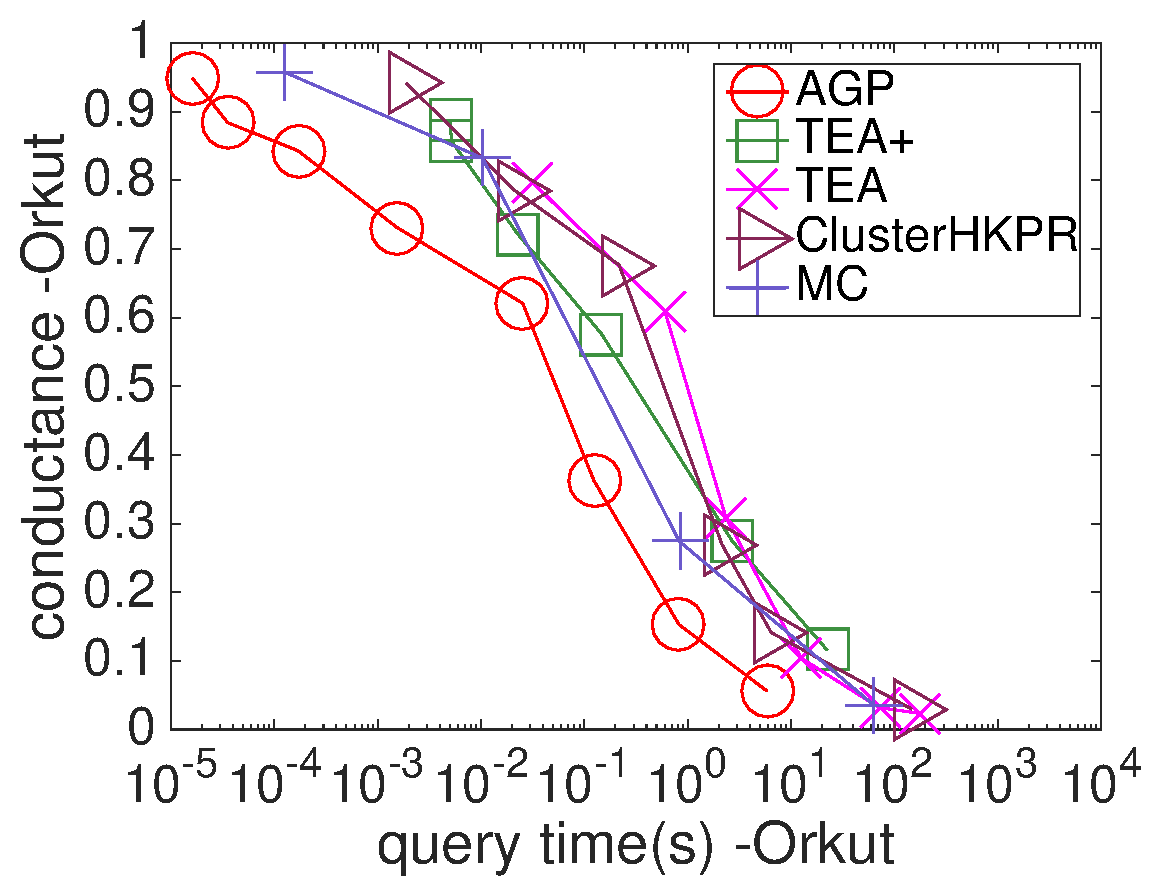
\includegraphics[height=34mm]{./Figs/HKPR-conductance-query-OL.eps} &
% 			\hspace{-4mm} 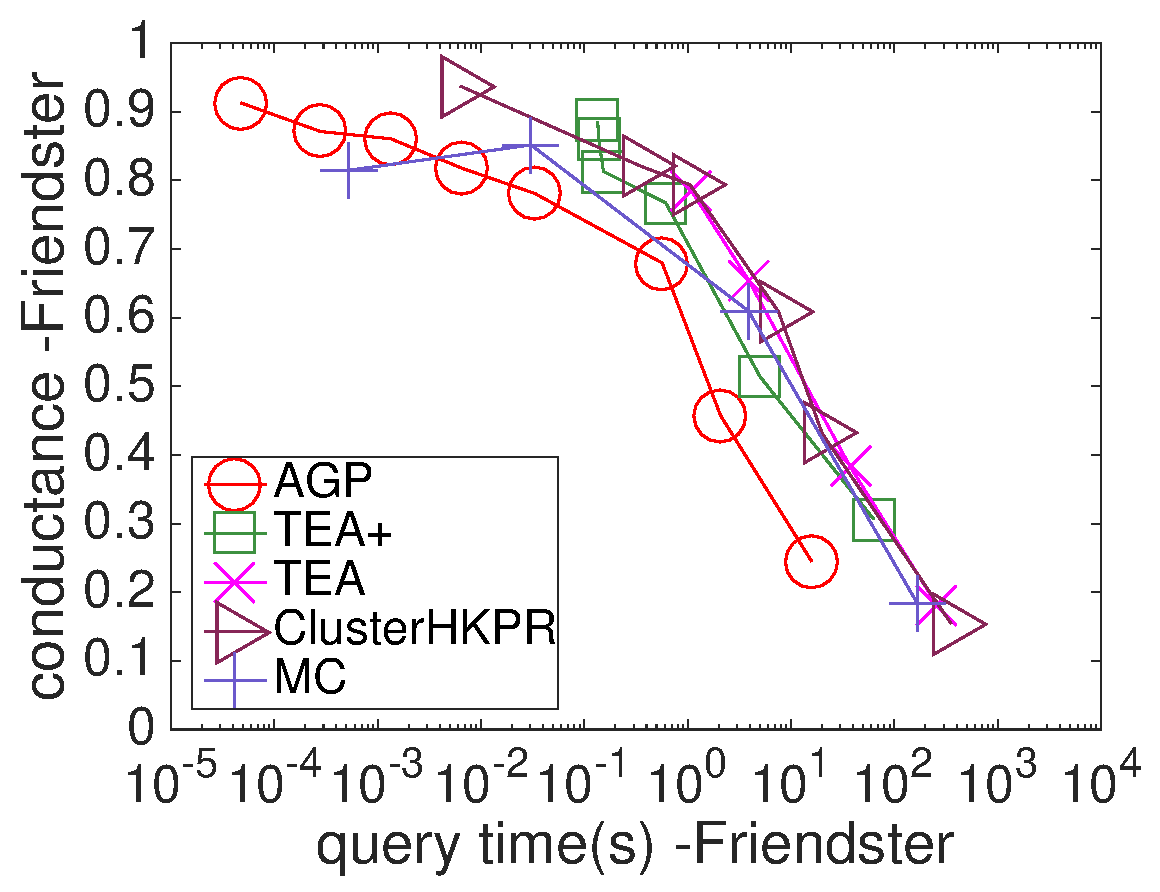
\includegraphics[height=34mm]{./Figs/HKPR-conductance-query-FR.eps} &
% 			%\hspace{-4mm} 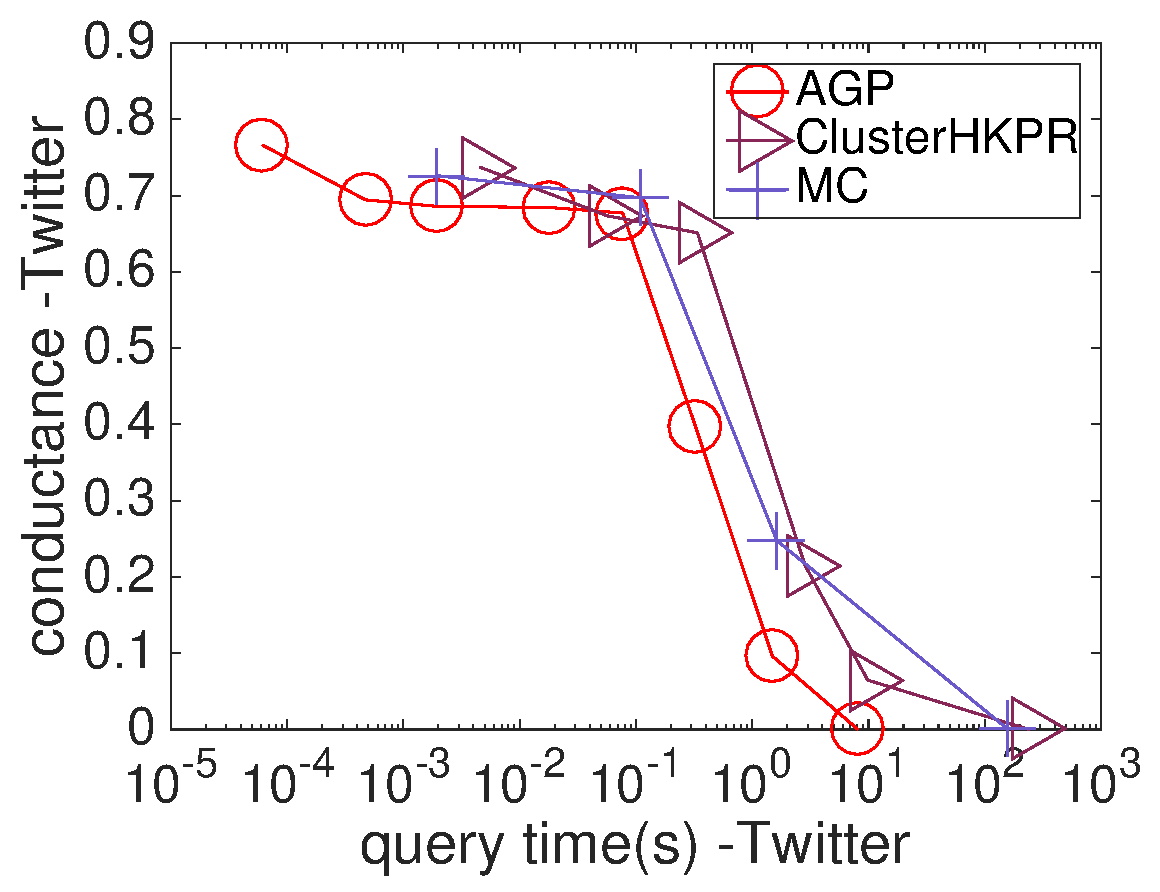
\includegraphics[height=34mm]{./Figs/HKPR-conductance-query-TW.eps} 
% 		\end{tabular}
% 		\vspace{-3mm}
% 		\caption{Tradeoffs between {\em conductance} and query time in local clustering.}
% 		\label{fig:HKPR-conductance-query}
% 		\vspace{-1mm}
% 	\end{small}
% \end{figure*}


\begin{figure*}[t]
	\begin{small}
		\centering
		%\vspace{-5mm}
		%    \begin{footnotesize}
		\begin{tabular}{cccc}
			%\multicolumn{4}{c}{\hspace{-4mm} \includegraphics[height=5mm]{./Figs/legend_large.eps}} \vspace{-1mm} \\
			%\hspace{-3mm} \includegraphics[height=25mm]{./Figs/HKPR-conductance-query-DB.eps} &
			\hspace{-4mm} 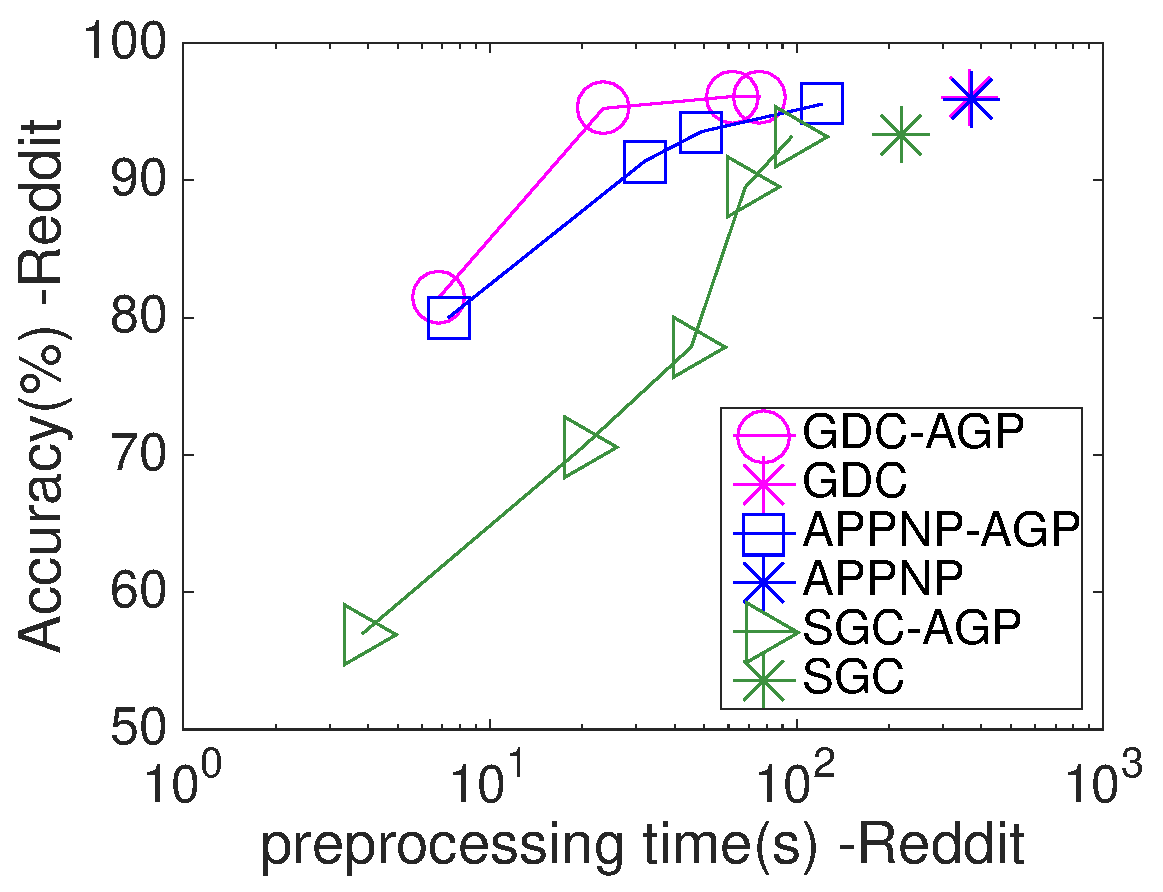
\includegraphics[height=34mm]{./Figs/GNN-accuracy-query-Reddit.eps} &
			\hspace{-4mm} 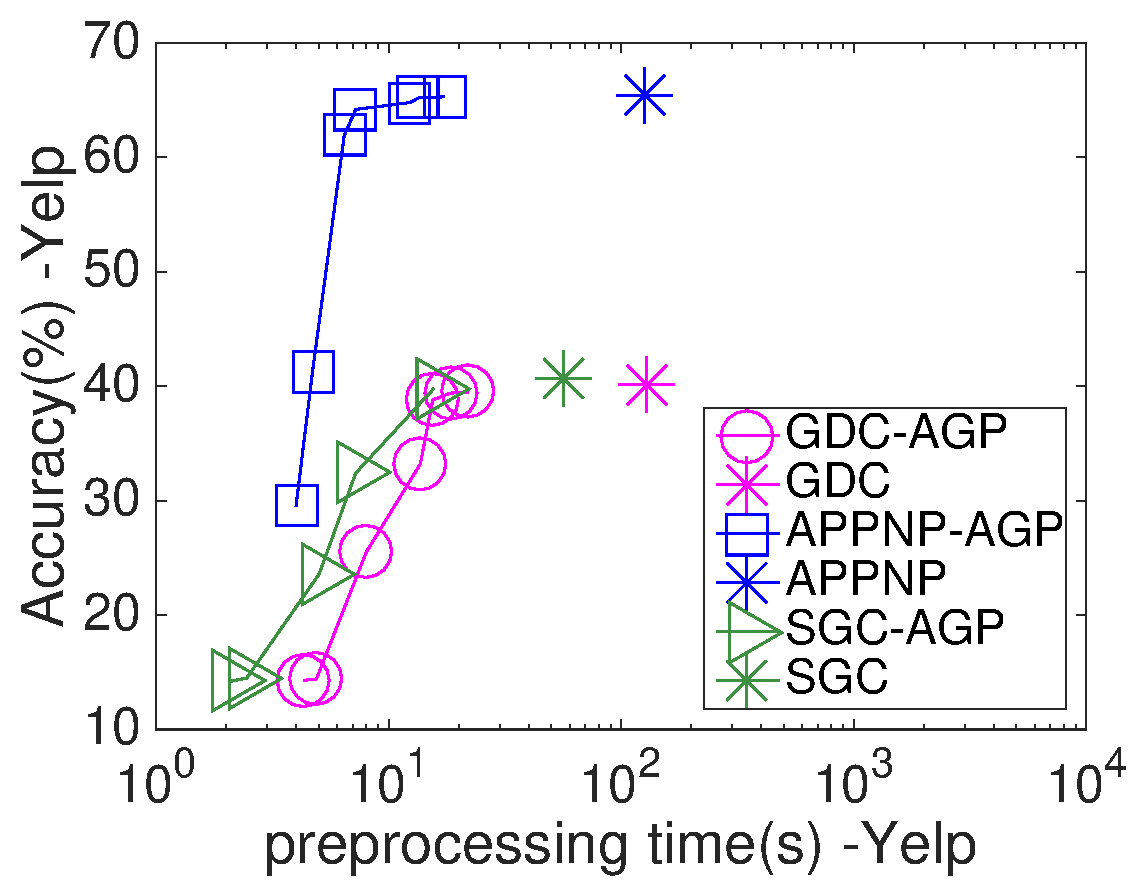
\includegraphics[height=34mm]{./Figs/GNN-accuracy-query-Yelp.eps} &
			\hspace{-2mm} \includegraphics[height=34mm]{./Figs/GNN-accuracy-query-Amazon.eps} &
			\hspace{-4mm} \includegraphics[height=34mm]{./Figs/GNN-accuracy-query-papers100M.eps} 
		\end{tabular}
		\vspace{-5mm}
		\caption{Tradeoffs between {\em Accuracy(\%)} and preprocessing time in node classification (Best viewed in color).}
		\label{fig:GNN-accuracy-query}
		\vspace{-2mm}
	\end{small}
\end{figure*}

\begin{figure}[t]
	\begin{small}
		\centering
		\vspace{-2mm}
		%    \begin{footnotesize}
		\begin{tabular}{cccc}
			%\multicolumn{4}{c}{\hspace{-4mm} \includegraphics[height=5mm]{./Figs/legend_large.eps}} \vspace{-1mm} \\
			%\hspace{-3mm} \includegraphics[height=25mm]{./Figs/HKPR-conductance-query-DB.eps} &
		%	\hspace{-4mm}  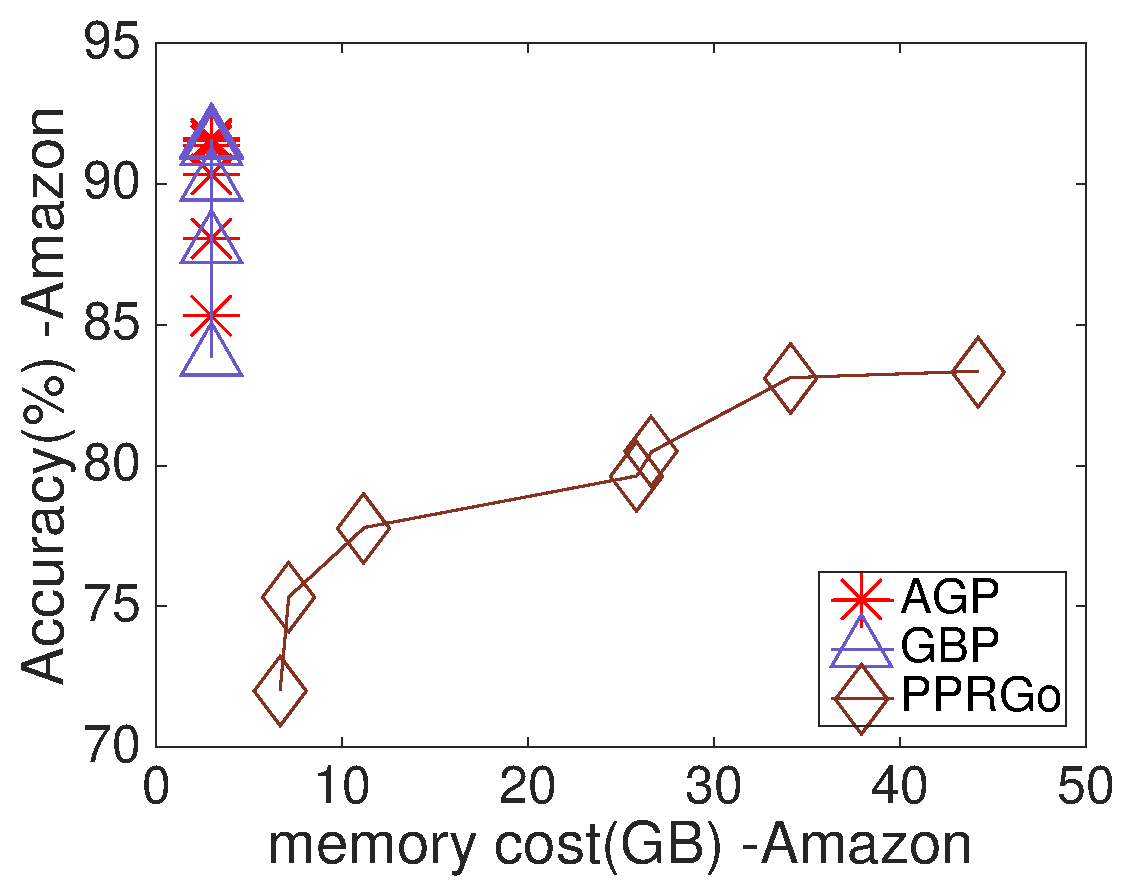
\includegraphics[height=34mm]{./Figs/GNN-accuracy-memory-Amazon.eps} &
			\hspace{-4mm}  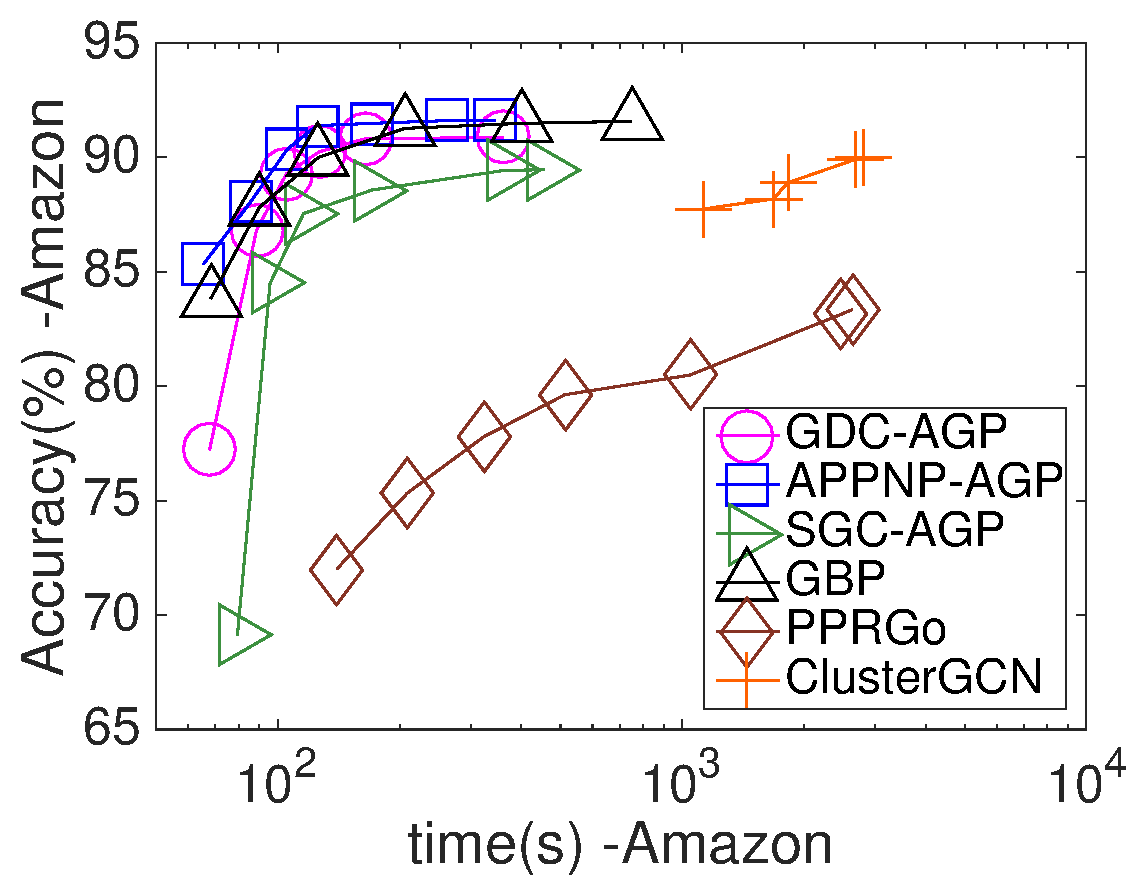
\includegraphics[height=32mm]{./Figs/GNN-accuracy-time-Amazon.eps} &
			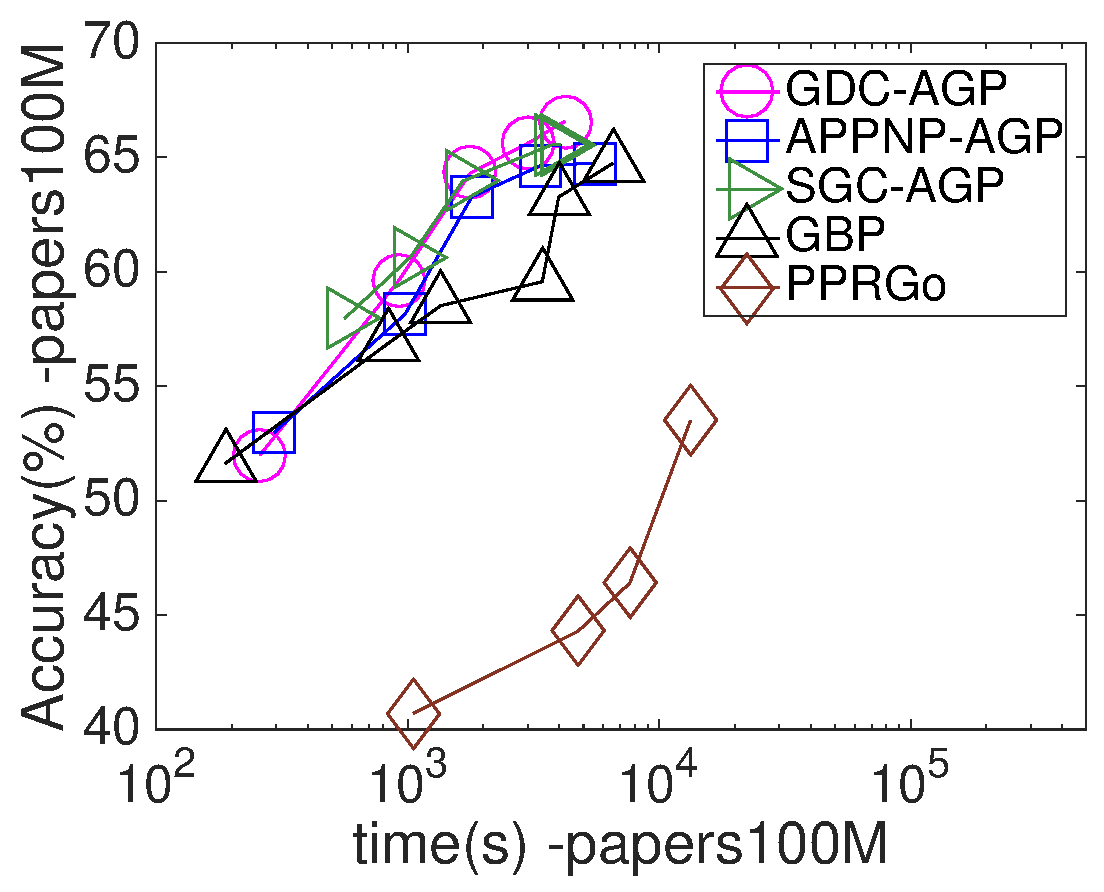
\includegraphics[height=32mm]{./Figs/GNN-accuracy-time-papers100M.eps}
		\end{tabular}
		\vspace{-5mm}
		\caption{Comparison with GBP, PPRGo and ClusterGCN.}
		\label{fig:GBP}
		\vspace{-5mm}
	\end{small}
\end{figure}



\vspace{-2mm}
\subsection{Local clustering with HKPR}\label{subsec:clustering}
In this subsection, we conduct experiments to evaluate the performance of AGP in local clustering problem. We select HKPR among various node proximity measures as it achieves the state-of-the-art result for local clustering~\cite{chung2018computing,kloster2014heat,yang2019TEA}. 
We will evaluate the trade-off curve between the query time and the approximation quality, as well as the trade-off curve between the query time and the clustering quality.
% first evaluate the query efficiency of heat kernel PageRank computed by AGP against other competitors. Then we compare the clustering quality of these methods using the derived HKPR results. Besides, we also exploit the influence of heat kernel parameter $t$ to the query effects of each algorithm. 




% choose one node proximity metric $\vec{\vec{\pi}}_s(t)$ first and approximate corresponding proximity results for each node $t \in V$ on the graph. 
% Next, sort the nodes on the graph in the descending order of $\frac{\vec{\pi}_s(t)}{d_t}$. 
% Finally, conduct the $\bf sweeping$ operation through the sorted nodes to find the subset with minimum conductance as the approximate clustering result. 
% In our experiments, we also obey this structure and apply heat kernel PageRank $\vec{\vec{\pi}}_s=\sum_{i=0}^\infty \frac{e^{-t}t^i}{i!}\cdot \left(\mathbf{A}\mathbf{D}^{-1}\right)^i\cdot \vec{e}_s$ as the node proximity following the state-of-the-art work~\cite{chung2018computing, kloster2014heat, yang2019TEA}. 


%normalize each proximity by
%Then they where heat kernel PageRank(HKPR) is the most commonly used proximity. 

%So in our experiments, we also compute the heat kernel PageRank first for every node on the graph with a given node as the seed. 





\header{\bf Datasets and Environment.} 
%Table~\ref{tbl:datasets} presents the detailed information of the datasets we used for local clustering, which can be obtained from~\cite{snapnets,LWA}. We use three undirected graphs: YouTube, Orkut, and Friendster in our experiments, as most of the local clustering methods can only support undirected graphs. We also use a large directed graph Twitter to demonstrate AGP's effectiveness on directed graphs. All local clustering experiments are conducted on a machine with an Intel(R) Xeon(R) Gold 6126@2.60GHz CPU and 500GB memory.
We use three undirected graphs: YouTube, Orkut, and Friendster in our experiments, as most of the local clustering methods can only support undirected graphs. We also use a large directed graph Twitter to demonstrate AGP's effectiveness on directed graphs. The four datasets can be obtained from~\cite{snapnets,LWA}. We summarize the detailed information of the four datasets in Table~\ref{tbl:datasets}. 



%\header{\bf Methods and Parameters.} 
\header{\bf Methods.} 
We compare AGP with four local clustering methods: TEA~\cite{yang2019TEA} and its optimized version TEA+, ClusterHKPR~\cite{chung2018computing}, and the Monte-Carlo method (MC). We use the results derived by the Basic Propagation Algorithm~\ref{alg:AGP-deter} with $L = 50$ as the ground truths for evaluating the trade-off curves of the approximate algorithms. Detailed descriptions on parameter setting for each method are deferred to appendix due to the space limits. 






\header{\bf Metrics.} 
%We use {\em MaxError} and {\em Precision@k} as our metrics to measure the approximation quality of each method. {\em MaxError} is defined as $MaxError =\max_{v \in V}\left|\frac{\vec{\pi}(v)}{d_v}-\frac{\vec{\epi}(v)}{d_v}\right|$, which measures the maximum error between the true normalized HKPR and the estimated value. Note that we use the basic propagation algorithm~\ref{alg:AGP-deter} with $L=50$ to obtain the ground truths of the normalized HKPR. 
We use {\em MaxError} as our metric to measure the approximation quality of each method. {\em MaxError} is defined as $MaxError =\max_{v \in V}\left|\frac{\vec{\pi}(v)}{d_v}-\frac{\vec{\epi}(v)}{d_v}\right|$, which measures the maximum error between the true normalized HKPR and the estimated value. We refer to $\frac{\vec{\pi}(v)}{d_{v}} $ as the {\em normalized HKPR} value from $s$ to $v$. %Note that we use the basic propagation algorithm~\ref{alg:AGP-deter} with $L=50$ to obtain the ground truths of the normalized HKPR.
On directed graph, $d_v$ is substituted by the out-degree $d_{out}(v)$. 
%We use {\em Precision@k} as our metric to measure the approximation quality of each method. Let $V_k$ denote the set of $k$ nodes with highest normalized HKPR values, and $\hat{V}_k$ denote the estimated top-$k$ node set returned by an approximate mthod. {\em Precision@k} is defined as the percentage of nodes in $\hat{V}_k$ that coincides with the actual top-$k$ results $V_k$. We use {\em Precision@k} to evaluate the accuracy of the relative node order of each method. We use the basic propagation algorithm~\ref{alg:AGP-deter} with $L=50$ to obtain the ground truths of the normalized HKPR. On directed graph, $d_t$ is substituted by the out-degree $d_{out}(v)$. 
 
%We also consider the quality of the cluster. More precisely, after deriving the (approximate )HKPR vector, we sort the nodes in descending order of the normalized HKPR values  and perform a sweeping operation to find the cluster with minimum conductance,  $\Phi(S)=\frac{|cut(S)|}{\min\{vol(S),2m-vol(S)\}}$ to measure the clustering quality, where $vol(S)=\sum_{v \in S}d(v)$, and $cut(S)=\{(u,v)\in E \mid u \in S, v \in V-S \}$. We evaluate the trade-offs between the minimum conductance found by each method and its query time. For each metric, we return the average of 50 randomly selected source nodes.  

%As mentioned in Section~\ref{subsec:cluserting-pre}, we perform local clustering methods with a sweeping algorithm. 
We also consider the quality of the cluster algorithms, which is measured by the {\em conductance}. Given a subset $S  \subseteq V$, the conductance is defined as $\Phi(S)\hspace{-1mm}=\hspace{-1mm}\frac{|cut(S)|}{\min\{vol(S),2m-vol(S)\}}$, where $vol(S)\hspace{-1mm}=\hspace{-1mm}\sum_{v \in S}d(v)$, and $cut(S)\hspace{-1mm}=\hspace{-1mm}\{(u,v)\hspace{-1mm}\in\hspace{-1mm} E \mid u \in S, v \in V-S \}$.
We perform a sweeping algorithm~\cite{Teng2004Nibble,FOCS06_FS,chung2007HKPR,chung2018computing,yang2019TEA} to find a subset $S$ with small conductance. More precisely, after deriving the (approximate) HKPR vector from a source node $s$, we sort the nodes $\{v_1, \ldots, v_n\}$ in descending order of the normalized HKPR values that $\frac{\vec{\pi}(v_1)}{d_{v_1}}\hspace{-1mm}\ge\hspace{-1mm} \frac{\vec{\pi}(v_2)}{d_{v_2}} \hspace{-1mm}\ge \hspace{-1mm}\ldots \hspace{-1mm}\ge \hspace{-1mm}\frac{\vec{\pi}(v_n)}{d_{v_n}}$. %we sort the nodes in descending order of the normalized HKPR values. 
Then, we sweep through $\{v_1, \ldots, v_n\}$ and find the node set with the minimum {\em conductance} among partial sets $S_i\hspace{-1mm} =\hspace{-1mm} \{v_1, \ldots,v_i\}, i\hspace{-1mm}=\hspace{-1mm}1,\ldots,n\hspace{-1mm}-\hspace{-1mm}1 $.

%More precisely, given a node $s$, we compute the HKPR vector $\vec{\pi} = \sum_{i=0}^\infty \frac{e^{-t}t^i}{i!}\cdot \left(\mathbf{A}\mathbf{D}^{-1}\right)^i\cdot \vec{e}_s$ of $s$, and sort the nodes $\{v_1, \ldots, v_n\}$ in descending order of $\frac{\vec{\pi}(v_1)}{d_{v_1}}\ge \frac{\vec{\pi}(v_2)}{d_{v_2}} \ge \ldots \ge \frac{\vec{\pi}(v_n)}{d_{v_n}}$. We refer to $\frac{\vec{\pi}(v)}{d_{v}} $ as the {\em normalized HKPR} value from $s$ to $v$. Then, we sweep through $\{v_1, \ldots, v_n\}$ and find the node set with the minimum conductance among partial sets $S_i = \{v_1, \ldots,v_i\}, i=1,\ldots,n-1 $. 
%After deriving the (approximate )HKPR vector, we perform a sweep algorithm to find the clusters with minimum conductance,  $\Phi(S)=\frac{|cut(S)|}{\min\{vol(S),2m-vol(S)\}}$ to measure the clustering quality, where $vol(S)=\sum_{v \in S}d(v)$, and $cut(S)=\{(u,v)\in E \mid u \in S, v \in V-S \}$. We evaluate the trade-offs between the minimum conductance found by each method and its query time. For each metric, we return the average of 50 randomly selected source nodes. 


 

\header{\bf Experimental Results.}
%Figure~\ref{fig:HKPR-precision-query} plots the trade-off curve between {\em Precision@50} and the query time for each method. We omit TEA and TEA+ on Twitter as they cannot handle directed graphs. We observe that AGP achieves the highest precision among the five approximate algorithms on all four datasets under the same query time. 
Figure~\ref{fig:HKPR-maxerror-query} plots the trade-off curve between the {\em MaxError} and query time. We observe that AGP  achieves the lowest curve among the five algorithms on all four datasets, which means AGP incurs the least error under the same query time. As a generalized algorithm for the graph propagation problem, these results suggest that AGP outperforms the state-of-the-art HKPR algorithms in terms of the approximation quality. 

% $1$ using the least time, which reflects the query efficiency of AGP. Besides, we notice that TEA+ and Monte-Carlo show a better performance than TEA and ClusterHKPR, which concurs with  analysis. In Figure~\ref{fig:HKPR-maxerror-query}, we plot the trade-offs between {\em MaxError} and query time. AGP is also the fastest method to reach the same additive error. Note that AGP can always achieve a $10x$ faster than TEA+ and $20\times-30\times$ faster than Monte-Carlo based methods. 
% Because the algorithm structure of TEA and TEA+ are only for undirected graphs. So we omit the lines of these two methods on the directed graph {\em Twitter}. On {\em Twitter}, AGP still has a better performance than the other Monte-Carlo based methods, which demonstrates the effectiveness of AGP on directed graphs. 

%To evaluate the quality of the clusters found by each method, Figure~\ref{fig:HKPR-conductance-query} shows the trade-off curve between conductance and the query time for each algorithm. We omit Twitter as the conductance metric which is only defined on undirected graphs.  We observe that AGP can achieve the lowest conductance-query time curve among the five approximate methods, which concurs that AGP provides estimators that are closest to the actual normalized HKPR. %ORIGIN!!
To evaluate the quality of the clusters found by each method, Figure~\ref{fig:HKPR-conductance-query} shows the trade-off curve between conductance and the query time on two large undirected graphs Orkut and Friendster. 
We observe that AGP can achieve the lowest conductance-query time curve among the five approximate methods on both of the two datasets, which concurs with the fact that AGP provides estimators that are closest to the actual normalized HKPR. 


%We also observe that as an exact algorithm, the basic propagation algorithm achieves the lowest conductance. 

%Finally,  Figure~\ref{fig:conductance-query-OL} plots the conductance and query time trade-offs on {\em Orkut}, with $t$ varying in $\{5,10,20,40\}$. Recall that $t$ is the average length of the heat kernel random walk. Hence, the query time of each method increases as  $t$ varying from 5 to 40.  We also observe that AGP consistently achieves the lowest conductance with the same amount of query time. Furthermore, as $t$ increases from $5$ to $40$, AGP's query time only increases by $7\times$, while TEA and TEA+ increase by $10\times-100\times$, which demonstrates the scalability of AGP. 

% the same conductance during the least time. Moreover, comparing the query time of each method when $t=5$ and $t=40$, AGP has a $7\times$ time increment, while $11\times$ increment for Monte-Carlo and $10-100\times$ increment for TEA+. This shows the good scalability of AGP. 





% \begin{table}[t]
% %\vspace{-5mm}
% 	\centering
% 	\tblcapup
% 	\caption{Comparison with APPNP, GDC and SGC.}
% 	\vspace{-3mm}
% 	\tblcapdown
% 	\begin{small}
% \begin{tabular}{|c|l|c|r|}
% \hline
% \multicolumn{2}{|c|}{}                  & \multicolumn{1}{l|}{Accuracy} & \multicolumn{1}{l|}{Propagation time(s)} \\ \hline
% \multirow{6}{*}{Amazon} & APPNP  & 91.4  & 454.1  \\ \cline{2-4}
%                 & AGP-APPNP      & 91.3  & 176.3  \\ \cline{2-4} 
%                         & GDC    & 90.8  & 458.2  \\ \cline{2-4}
%                 & AGP-GDC        & 90.8  & 114.7  \\ \cline{2-4}
%                         & SGC    & 89.5  & 271.8  \\ \cline{2-4} 
%                 & AGP-SGC        & 88.9  & 93.6   \\ \hline
                
% \multirow{6}{*}{Yelp} & APPNP    & 65.4  & 127.4  \\ \cline{2-4}
%                 & AGP-APPNP      & 65.4  & 17.3   \\ \cline{2-4}
%                       & GDC      & 39.6  & 129.8  \\ \cline{2-4}
%                 & AGP-GDC        & 39.5  & 18.4   \\ \cline{2-4}
%                       & SGC      & 30.1  & 56.7   \\ \cline{2-4} 
%                 & AGP-SGC        & 29.8  & 15.6   \\ \hline
                
% \multirow{6}{*}{Reddit} & APPNP  & 95.9  & 366.1  \\ \cline{2-4}
%                 & AGP-APPNP      & 95.7  & 87.1   \\ \cline{2-4}
%                         & GDC    & 96.1  & 367.7  \\ \cline{2-4}
%                 & AGP-GDC        & 96.1  & 62.1   \\ \cline{2-4}
%                         & SGC    & 93.5  & 161.4  \\ \cline{2-4} 
%                 & AGP-SGC        & 93.2  & 86.3   \\ \hline
                
% \multirow{6}{*}{Papers100M} 
%                       & APPNP    & 62.3  & 55706.8   \\ \cline{2-4}
%                 & AGP-APPNP       & 62.2  & 9253.7    \\ \cline{2-4}
%                       & GDC      & 64.3  & 51247.1   \\ \cline{2-4}
%                 & AGP-GDC         & 64.1  & 6808.2    \\ \cline{2-4}
%                       & SGC      & 63.4  & 24968.6   \\ \cline{2-4}
%                 & AGP-SGC         & 61.2  & 1437.2    \\ \hline
% \end{tabular}
% \end{small}
% \end{table}


\begin{table}[t]
	\vspace{-3mm}
	\centering
	\tblcapup
	\caption{Datasets for node classification.}
	\vspace{-5mm}
	\tblcapdown
	\begin{small}
		\begin{tabular}{|l|r|r|r|r|r|} %p{1.3in}|}
			\hline
			{\bf Data Set} & {\bf $\boldsymbol{n}$}& {\bf $\boldsymbol{m}$} & {\bf $\boldsymbol{d}$}& {\bf Classes} 	& {\bf Label $\%$}  \\ \hline
    Reddit     & 232,965 &   114,615,892 &602 & 41  & 0.0035           \\
    Yelp        & 716,847     & 6,977,410   & 300 & 100 & 0.7500         \\
    Amazon        & 2,449,029   & 61,859,140  & 100   & 47 & 0.7000      \\
    Papers100M     & 111,059,956 & 1,615,685,872  & 128  &  172 & 0.0109           \\
			\hline
		\end{tabular}
	\end{small}
	\label{tbl:datasets_gnn}
	%\tbldown
	\vspace{-6mm}
\end{table}

\vspace{-2mm}
\subsection{Node classification with GNN}\label{subsec:GNN}
In this section, we evaluate the AGP's ability to scale  existing Graph Neural Network models on large graphs.

\header{\bf Datasets.}
%We use four publicly available graph datasets with different size: a socal network Reddit~\cite{hamilton2017graphSAGE}, a customer interaction network Yelp~\cite{zeng2019graphsaint}, a co-purchasing network Amazon~\cite{chiang2019clusterGCN} and a large citation network Papers100M~\cite{hu2020ogb}. Table~\ref{tbl:datasets_gnn} summarizes the statistics of the datasets. Note that $d$ is the dimension of the node feature, and the label rate is the percentage of labeled nodes in the graph. Following~\cite{zeng2019graphsaint,zou2019layer}, we perform inductive node classification on Yelp, Amazon and Reddit, and semi-supervised transductive node classification on Papers100M. More specifically, for inductive node classification tasks, we train the model on a graph with labeled nodes and predict nodes' labels on a testing graph. For semi-supervised transductive node classification tasks, we train the model with a small subset of labeled nodes and predict other nodes' labels in the same graph. We follow the same training/validation/testing split as previous works in GNN~\cite{zeng2019graphsaint,hu2020ogb}. A detailed discussion on the setting of the experiments can be found in the appendix.
We use four publicly available graph datasets with different size: a socal network Reddit~\cite{hamilton2017graphSAGE}, a customer interaction network Yelp~\cite{zeng2019graphsaint}, a co-purchasing network Amazon~\cite{chiang2019clusterGCN} and a large citation network Papers100M~\cite{hu2020ogb}. Table~\ref{tbl:datasets_gnn} summarizes the statistics of the datasets, where $d$ is the dimension of the node feature, and the label rate is the percentage of labeled nodes in the graph. A detailed discussion on datasets can be found in the appendix. 


% We first evaluate GBP's performance for transductive semi-supervised learning on the three popular citation networks (Cora, Citeseer, and Pubmed). Then we compare GBP with scalable GNN methods three medium to large graphs PPI, Yelp, Amazon in terms of inductive learning ability. Finally, we present the first empirical study of transductive semi-supervised on billion-scale network Friendster. 


%\header{\bf GNN models and detailed setup.} 
\header{\bf GNN models.} 
%%We consider three proximity-based GNN models: APPNP~\cite{Klicpera2018APPNP}, SGC~\cite{wu2019SGC}, and GDC~\cite{klicpera2019GDC}. We augment the three models with the AGP algorithm~\ref{alg:AGP-RQ} to obtain three variants: APPNP-AGP, SGC-AGP and GDC-AGP. Take SGC-AGP as an example. Recall that SGC uses $\mathbf{Z}= \left(\mathbf{D}^{-\frac{1}{2}} \mathbf{A}\mathbf{D}^{-\frac{1}{2}} \right)^L \cdot \X$ to perform feature aggregation, where $\vec{X}$ is the $n\times d$ feature matrix. SGC-AGP treats each column of $\vec{X}$ as a graph signal $\vec{x}$ and perform randomized propagation algorithm (Algorithm~\ref{alg:AGP-RQ}) with predetermined error parameter $\delta$ to obtain the the final representation $\mathbf{Z}$. To achieve high parallelism, we perform propagation for multiple columns of $\mathbf{X}$ in parallel. 
We first consider three proximity-based GNN models: APPNP~\cite{Klicpera2018APPNP},SGC~\cite{wu2019SGC}, and GDC~\cite{klicpera2019GDC}. We augment the three models with the AGP Algorithm~\ref{alg:AGP-RQ} to obtain three variants: APPNP-AGP, SGC-AGP and GDC-AGP. Besides, we also compare AGP with three scalable methods: PPRGo~\cite{bojchevski2020scaling}, GBP~\cite{chen2020GBP}, and ClusterGCN~\cite{chiang2019clusterGCN}. 


%We first consider three proximity-based GNN models: APPNP~\cite{Klicpera2018APPNP},SGC~\cite{wu2019SGC}, and GDC~\cite{klicpera2019GDC}. We augment the three models with the AGP Algorithm~\ref{alg:AGP-RQ} to obtain three variants: APPNP-AGP, SGC-AGP and GDC-AGP. Take SGC-AGP as an example. Recall that SGC uses $\mathbf{Z}=\left(\mathbf{D}^{-\frac{1}{2}} \mathbf{A}\mathbf{D}^{-\frac{1}{2}} \right)^L \hspace{-1mm}\cdot \X$ to perform feature aggregation, where $\X$ is the $n\times d$ feature matrix. SGC-AGP treats each column of $\X$ as a graph signal $\bm{x}$ and perform randomized propagation algorithm (Algorithm~\ref{alg:AGP-RQ}) with predetermined error parameter $\delta$ to obtain the the final representation $\mathbf{Z}$. To achieve high parallelism, we perform propagation for multiple columns of $\mathbf{X}$ in parallel. Since APPNP and GDC's original implementation cannot scale on billion-edge graph Papers100M, we implement APPNP and GDC in the AGP framework. In particular, we set $\varepsilon = 0$ in Algorithm~\ref{alg:AGP-RQ} to obtain the exact propagation matrix $\mathbf{Z}$, in which case the approximate models APPNP-AGP and GDC-AGP essentially become the exact models APPNP and GDC. We set $L\hspace{-1mm}=\hspace{-1mm}20$ for GDC-AGP and APPNP-AGP, and $L\hspace{-1mm}=\hspace{-1mm}10$ for SGC-AGP. Note that SGC suffers from the over-smoothing problem when the number of layers $L$ is large~\cite{wu2019SGC}. We vary the parameter $\varepsilon$ to obtain a trade-off curve between the classification accuracy and the computation time. 


%%Finally, we also include PPRGo~\cite{bojchevski2020scaling}, the state-of-the-art method that improves the scalability of APPNP. PPRGo has three main parameters: the number of non-zero PPR values for each training node $k$, the number of hops $L$, and the residue threshold $r_{max}$. We vary the three parameters $(k, L, r_{max})$ to form a trade-off curve between the classification accuracy and the computation time. 

%Besides, we also compare AGP with three scalable methods: PPRGo~\cite{bojchevski2020scaling}, GBP~\cite{chen2020GBP}, and ClusterGCN~\cite{chiang2019clusterGCN}. Recall that PPRGo is an improvement work of APPNP. It has three main parameters: the number of non-zero PPR values for each training node $k$, the number of hops $L$, and the residue threshold $r_{max}$. %We vary the three parameters $(k, L, r_{max})$ to form a trade-off curve between the classification accuracy and the computation time. We vary the three parameters $(k,L,r_{max})$ from $(32,2,0.1)$ to $(64,10,10^{-5})$. GBP decouples the feature propagation and prediction to achieve high scalability. In the propagation process, GBP has two parameters: the propagation threshold $r_{max}$ and the level $L$. We vary $r_{max}$ from $10^{-4}$ to $10^{-10}$, and set $L=4$. ClusterGCN uses graph sampling method to partition graphs into small parts, and performs the feature propagation on one randomly picked sub-graph in each mini-batch. We vary the partition numbers from $10^4$ to $10^5$, and the propagation layers from $2$ to $4$. For AGP, we vary $\delta$ from $10^{-5}$ to $10^{-10}$, and tune $a,b,w_i$ for the best performance. %Detailed parameter settings can be founded in the appendix. 


%%For each method, we apply a neural network with two hidden layers, trained with mini-batch SGD. The batch size is set to be $10000$ for faster training time and better generalization ability. We employ initial residual connection~\cite{He2016ResNet} across the hidden layers to facilitate training. We use the trained model to predict each testing node's labels and take the mean accuracy after five runs. For each method, we divide the computation time into two parts: the {\em propagation time} for computing $\mathbf{Z}$, and the {\em training time} for performing mini-batch SGD on the 2-layer neural network on $\mathbf{Z}$ until convergence.


%For each method, we apply a neural network with 4 hidden layers, trained with mini-batch SGD. %The batch size is set to be $10000$ for faster training time and better generalization ability. We employ initial residual connection~\cite{He2016ResNet} across the hidden layers to facilitate training. We use the trained model to predict each testing node's labels and take the mean accuracy after five runs. For GDC, APPNP, and SGC, we divide the computation time into two parts: the {\em preprocessing time} for computing $\mathbf{Z}$, and the {\em training time} for performing mini-batch SGD on $\mathbf{Z}$ until convergence. 



\header{\bf Experimental results.} Figure~\ref{fig:GNN-accuracy-query} shows the trade-off between the preprocessing time and classification accuracy for SGC, APPNP, GDC and the corresponding AGP models. For each dataset, the three snowflakes represent the exact methods SGC, APPNP, and GDC, which can be distinguished by colors.
We observe that compared to the exact models, the approximate models generally achieve a $10\times$ speedup in preprocessing time without sacrificing the classification accuracy. For example, on the billion-edge graph Papers100M,  SGC-AGP achieves an accuracy of $62\%$ in less than $2,000$ seconds, while the exact model SGC needs over $20,000$ seconds to finish. %We also observe that APPNP-AGP achieves a higher trade-off curve than PPRGo does, which means AGP is more efficient than PPRGo in terms of scaling PPR-based GNN on large graphs. %To eliminate the effect of parallelism, we also present each method's clock time in the appendix of the technical report~\cite{TechnicalReport} . The results concur with what we found in Figure~\ref{fig:GNN-accuracy-query}. 

Figure~\ref{fig:GBP} shows the performances of AGP compared with PPRGo, GBP, and ClusterGCN on Amazon and Papers100M, the largest publicly available graphs for inductive and transductive node classification tasks, respectively.
We present the trade-off plots between the total computation time and classification accuracy for each model. We report the total running time (i.e., preprocessing time plus training time). 

We omit ClusterGCN on Papers100M as it runs out of 512GB memory on this graph. We observe that AGP significantly outperforms PPRGo and ClusterGCN on both Amazon and Papers100M in terms of both accuracy and running time. Furthermore, given the same running time, AGP achieves a higher accuracy than GBP does on Papers100M. We attribute this quality to the randomization introduced in AGP.





%Figure~\ref{fig:GNN-accuracy-memory} shows the memory overhead of each approximate method. Recall that the AGP algorithm~\ref{alg:AGP-RQ} only maintains two $n$ dimension vectors: the residue vector $\vec{r}$ and the reserve vector $\vec{q}$. Consequently, AGP only takes a fixed memory, which can be ignored compared to the graph's size and the feature matrix.  Such property is ideal for scaling GNN models on massive graphs. On the other hand, PPRGo requires a large memory size to store the intermediate local push results from each training node.






 % Besides, it set the maximum length of walk as $K=t\cdot \frac{\log{1/\delta}}{\log{\log{1/\delta}}}$. When the poisson random number $k$ is large than $K$, it truncate the walk at its $K_{th}$ step. For ClusterHKPR, 
% To obtain a tradeoff curve between the approximation quality and query time, we vary $\delta$ from $0.5$ to $0.0001$ in our experiments. 
%and generate $\frac{16\log{n}}{\delta^2 }$ walks from the seed, instead of $$. 
%evaluates the performance of AGP against state-of-the-art methods.


%%% Local Variables:
%%% mode: latex
%%% TeX-master: "paper"
%%% End:

\vspace{-2mm}
\section{Conclusion} \label{sec:conclusion}
\vspace{-1mm}
In this paper, we propose the concept of approximate graph propagation, which unifies various proximity measures, including transition probabilities, PageRank and Personalized PageRank, heat kernel PageRank, and Katz. We present a randomized graph propagation algorithm that achieves almost optimal computation time with a theoretical error guarantee. We conduct an extensive experimental study to demonstrate the effectiveness of AGP on real-world graphs. We show that AGP outperforms the state-of-the-art algorithms in the specific application of local clustering and node classification with GNNs. For future work, it is interesting to see if the AGP framework can inspire new proximity measures for graph learning and mining tasks.

\vspace{-1mm}



%%% Local Variables:
%%% mode: latex
%%% TeX-master: "paper"
%%% End:

\section{ACKNOWLEDGEMENTS}
Zhewei Wei was supported by National Natural Science Foundation of China (NSFC) No. 61972401 and No. 61932001, by the Fundamental Research Funds for the Central Universities and the Research Funds of Renmin University of China under Grant 18XNLG21, and by Alibaba Group through Alibaba Innovative Research Program. 
Hanzhi Wang was supported by the Outstanding Innovative Talents Cultivation Funded Programs 2020 of Renmin Univertity of China.
Sibo Wang was supported by Hong Kong RGC ECS No. 24203419, RGC CRF No. C4158-20G, and NSFC No. U1936205. 
Ye Yuan was supported by NSFC No. 61932004 and No. 61622202, and by FRFCU No. N181605012. 
Xiaoyong Du was supported by NSFC No. 62072458. 
Ji-Rong Wen was supported by NSFC  No. 61832017, and by Beijing Outstanding Young Scientist Program NO. BJJWZYJH012019100020098. 
This work was supported by Public Computing Cloud, Renmin University of China.

%This research was supported in part by National Natural Science Foundation of China (No. 61832017, No. 61972401, No. 61932001, No. U1711261, No. 61932004 and No. 61622202), by FRFCU No. N181605012, by Beijing Outstanding Young Scientist Program NO. BJJ WZYJH012019100020098, and by the Fundamental Research Funds for the Central Universities and the Research Funds of Renmin University of China under Grant 18XNLG21.

%%% Local Variables:
%%% mode: latex
%%% TeX-master: "paper"
%%% End:


%%
%% The next two lines define the bibliography style to be used, and
%% the bibliography file.

\balance
%\bibliographystyle{ACM-Reference-Format}
\bibliographystyle{plain}
\bibliography{paper}

%%
%% If your work has an appendix, this is the place to put it.


\appendix
%\clearpage
\begin{table*}[t]
	%\vspace{-1mm}
	%\centering
	%\lefting
	\tblcapup
	\caption{Hyper-parameters of AGP.}
	\vspace{-5mm}
	\tblcapdown
	\begin{small}
	\begin{threeparttable}
		\begin{tabular}{|c|c|c|c|c|c|c|c|c|c|c|}
			\hline
			\multirow{2}{*}{{\bf Data set}} & \multirow{2}{*}{\bf Learning rate}& \multirow{2}{*}{{\bf Dropout}} & {\bf Hidden} &\multirow{2}{*}{\bf Batch size} & {\bf GDC-AGP}&{\bf APPNP-AGP}&\bf SGC-AGP &\multicolumn{3}{c|}{\bf AGP} \\ \cline{6-11}
			~&&&{\bf dimension} & &$\boldsymbol{t}$& $\boldsymbol{\alpha}$& $\boldsymbol{L}$& {\bf $a$} &{\bf $b$}& {\bf $w_i$} \\ \hline
Yelp & 0.01 & 0.1 & 2048 & $3\cdot 10^4$&  4 & 0.9& 10 & - & - & -\\
Amazon  & 0.01 & 0.1 & 1024 &$10^5$& 4 & 0.2& 10 & 0.8 & 0.2 & $\alpha(1-\alpha)^i, \alpha=0.2$\\
Reddit  & 0.0001 & 0.3 &  2048  &$10^4$& 3 & 0.1& 10 & - & -& -\\
Papers100M & 0.0001 & 0.3 & 2048 &$10^4$& 4 & 0.2& 10 & 0.5 & 0.5 & $e^{-t}\cdot \frac{t^i}{i!}, t=4$\\ 
			\hline
		\end{tabular}
	\end{threeparttable}
	\end{small}
	\label{tbl:parameters}
	%\tbldown
	\vspace{-1mm}
\end{table*}

\section{Additional Experimental Descriptions}\label{sec:appendix}

\subsection{Local clustering with HKPR}

\header{\bf Methods and Parameters. }
For our method, we set $a=0,b=1, w_i=\frac{e^{-t}t^i}{i!}$, and $\vec{x}=\vec{e}_s$ in Equation~\eqref{eqn:pi_gen} to simulate the HKPR equation $\vec{\pi}=\sum_{i=0}^\infty \frac{e^{-t}t^i}{i!}\cdot \left(\mathbf{A}\mathbf{D}^{-1}\right)^i\cdot \vec{e}_s$. We employ the randomized propagation algorithm~\ref{alg:AGP-RQ} with level number $L= O\left(\log {1/\delta}\right)$ and error parameter $\varepsilon = \frac{2\delta}{L(L+1)}$, where $\delta$ is the relative error threshold in Definition~\ref{def:pro-relative}. We use AGP to denote this method. We vary $\delta$ from $0.1$ to $10^{-8}$ to obtain a trade-off curve between the approximation quality and the query time. 
%We also include the basic propagation algorithm~\ref{alg:AGP-deter} with $L = 50$ (denoted as Basic), which serves as the algorithm for computing ground and as a baseline for evaluating the trade-off curves of the approximate algorithms.
We use the results derived by the Basic Propagation Algorithm~\ref{alg:AGP-deter} with $L = 50$ as the ground truths for evaluating the trade-off curves of the approximate algorithms.

We compare AGP with four local clustering methods: TEA~\cite{yang2019TEA} and its optimized version TEA+, ClusterHKPR~\cite{chung2018computing}, and the Monte-Carlo method (MC). 
TEA~\cite{yang2019TEA}, as the state-of-the-art clustering method, combines a deterministic push process with the Monte-Carlo random walk. Given a graph $G=(V, E)$, and a seed node $s$, TEA conducts a local search algorithm to explore the graph around $s$ deterministically, and then generates random walks from nodes with residues exceeding a threshold parameter $r_{max}$.  One can manipulate $r_{max}$ to balance the two processes. It is shown in~\cite{yang2019TEA} that TEA can achieve $O\left(\frac{t\cdot \log{n}}{\delta}\right)$ time complexity, where $t$ is the constant heat kernel parameter.
ClusterHKPR~\cite{chung2018computing} is a Monte-Carlo based method that simulates adequate random walks from the given seed node and uses the percentage of random walks terminating at node $v$ as the estimation of $\vec{\pi}(v)$. 
%In the $k_{th}$ step, the walk stops at the node it currently walks at with the probability , or move to a randomly selected neighbor with the probability $\frac{t}{k}$. 
The length of walks $k$ follows the Poisson distribution $\frac{e^{-t}t^k}{k!}$. The number of random walks need to achieve a relative error of $\delta$ in Definition~\ref{def:pro-relative} is $O\left(\frac{t\cdot \log{n}}{\delta^3}\right)$. 
MC~\cite{yang2019TEA} is an optimized version of random walk process that sets identical length for each walk as $L=t\cdot \frac{\log{1/\delta}}{\log{\log{1/\delta}}}$. If a random walk visit node $v$ at the $k$-th step,  we add $\frac{e^{-t}t^k}{n_r \cdot k!}$ to the propagation results $\vec{\epi}(v)$, where $n_r$ denotes the total number of random walks. The number of random walks to achieve a relative error of $\delta$ is also $O\left(\frac{t\cdot \log{n}}{\delta^3}\right)$. Similar to AGP, for each method, we vary $\delta$ from $0.1$ to $10^{-8}$ to obtain a trade-off curve between the approximation quality and the query time. 
Unless specified otherwise, we set the heat kernel parameter $t$ as 5, following~\cite{kloster2014heat, yang2019TEA}. All local clustering experiments are conducted on a machine with an Intel(R) Xeon(R) Gold 6126@2.60GHz CPU and 500GB memory. 


\subsection{Node classification with GNN}

\header{\bf Datasets. }
Following~\cite{zeng2019graphsaint,zou2019layer}, we perform inductive node classification on Yelp, Amazon and Reddit, and semi-supervised transductive node classification on Papers100M. More specifically, for inductive node classification tasks, we train the model on a graph with labeled nodes and predict nodes' labels on a testing graph. For semi-supervised transductive node classification tasks, we train the model with a small subset of labeled nodes and predict other nodes' labels in the same graph. We follow the same training/validation/test-ing split as previous works in GNN~\cite{zeng2019graphsaint,hu2020ogb}. 





\header{\bf GNN models.} 
We first consider three proximity-based GNN models: APPNP~\cite{Klicpera2018APPNP},SGC~\cite{wu2019SGC}, and GDC~\cite{klicpera2019GDC}. We augment the three models with the AGP Algorithm~\ref{alg:AGP-RQ} to obtain three variants: APPNP-AGP, SGC-AGP and GDC-AGP. Take SGC-AGP as an example. Recall that SGC uses $\mathbf{Z}=\left(\mathbf{D}^{-\frac{1}{2}} \mathbf{A}\mathbf{D}^{-\frac{1}{2}} \right)^L \hspace{-1mm}\cdot \X$ to perform feature aggregation, where $\X$ is the $n\times d$ feature matrix. SGC-AGP treats each column of $\X$ as a graph signal $\bm{x}$ and perform randomized propagation algorithm (Algorithm~\ref{alg:AGP-RQ}) with predetermined error parameter $\delta$ to obtain the the final representation $\mathbf{Z}$. To achieve high parallelism, we perform propagation for multiple columns of $\mathbf{X}$ in parallel. Since APPNP and GDC's original implementation cannot scale on billion-edge graph Papers100M, we implement APPNP and GDC in the AGP framework. In particular, we set $\varepsilon = 0$ in Algorithm~\ref{alg:AGP-RQ} to obtain the exact propagation matrix $\mathbf{Z}$, in which case the approximate models APPNP-AGP and GDC-AGP essentially become the exact models APPNP and GDC. We set $L\hspace{-1mm}=\hspace{-1mm}20$ for GDC-AGP and APPNP-AGP, and $L\hspace{-1mm}=\hspace{-1mm}10$ for SGC-AGP. Note that SGC suffers from the over-smoothing problem when the number of layers $L$ is large~\cite{wu2019SGC}. We vary the parameter $\varepsilon$ to obtain a trade-off curve between the classification accuracy and the computation time. 

\begin{table}[t]
	%\vspace{-2mm}
	%\centering
	%\lefting
	\tblcapup
	\caption{URLs of baseline codes.}
	\vspace{-3mm}
	\tblcapdown
	\begin{small}
		%\begin{tabular}{|c|c|c|} %p{1.3in}|}
			
		\begin{tabular}{|c|c|}\hline
	%{\bf Methods} & {\bf URL} & \hspace{-2mm}{\bf Commit}\hspace{-5mm}\\ \hline
    %GDC & https://github.com/klicperajo/gdc & \hspace{-2mm}14333fd\hspace{-2mm}\\
    %APPNP & https://github.com/rusty1s/pytorch$\_$geometric & \hspace{-2mm}f560655\hspace{-2mm}\\
    %SGC & https://github.com/Tiiiger/SGC &\hspace{-2mm}795ec93 \hspace{-2mm} \\ 
    %PPRGo & https://github.com/TUM-DAML/pprgo$\_$pytorch &\hspace{-2mm} d9f991e\hspace{-2mm}\\ 
    %GBP & https://github.com/chennnM/GBP &\hspace{-2mm}f811fc2 \\
    %\hspace{-2mm}ClusterGCN\hspace{-2mm} &\hspace{-2mm}https://github.com/benedekrozemberczki/ClusterGCN \hspace{-2mm} &\hspace{-2mm}a6b40cc\hspace{-2mm} \\ \hline
    {\bf Methods} & {\bf URL} \\ \hline
    GDC & https://github.com/klicperajo/gdc \\
    APPNP & https://github.com/rusty1s/pytorch$\_$geometric \\
    SGC & https://github.com/Tiiiger/SGC \\ 
    PPRGo & https://github.com/TUM-DAML/pprgo$\_$pytorch \\ 
    GBP & https://github.com/chennnM/GBP \\ 
    ClusterGCN &https://github.com/benedekrozemberczki/ClusterGCN \\ \hline
	\end{tabular}
	\end{small}
	\label{tbl:url}
	%\tbldown
	%\vspace{-2mm}
\end{table}


Besides, we also compare AGP with three scalable methods: PPRGo~\cite{bojchevski2020scaling}, GBP~\cite{chen2020GBP}, and ClusterGCN~\cite{chiang2019clusterGCN}. Recall that PPRGo is an improvement work of APPNP. It has three main parameters: the number of non-zero PPR values for each training node $k$, the number of hops $L$, and the residue threshold $r_{max}$. We vary the three parameters $(k,L,r_{max})$ from $(32,2,0.1)$ to $(64,10,10^{-5})$. GBP decouples the feature propagation and prediction to achieve high scalability. In the propagation process, GBP has two parameters: the propagation threshold $r_{max}$ and the level $L$. We vary $r_{max}$ from $10^{-4}$ to $10^{-10}$, and set $L=4$ following~\cite{chen2020GBP}. ClusterGCN uses graph sampling method to partition graphs into small parts, and performs the feature propagation on one randomly picked sub-graph in each mini-batch. We vary the partition numbers from $10^4$ to $10^5$, and the propagation layers from $2$ to $4$. For AGP, we vary $\delta$ from $10^{-5}$ to $10^{-10}$, and tune $a,b,w_i$ for the best performance. 

For each method, we apply a neural network with 4 hidden layers, trained with mini-batch SGD. %The batch size is set to be $10000$ for faster training time and better generalization ability.
We employ initial residual connection~\cite{He2016ResNet} across the hidden layers to facilitate training. We use the trained model to predict each testing node's labels and take the mean accuracy after five runs. For GDC, APPNP, and SGC, we divide the computation time into two parts: the {\em preprocessing time} for computing $\mathbf{Z}$, and the {\em training time} for performing mini-batch SGD on $\mathbf{Z}$ until convergence. All the experiments in this section are conducted on a machine with an NVIDIA RTX8000 GPU (48GB memory), Intel Xeon CPU (2.20 GHz) with 40 cores, and 512 GB of RAM. Detailed parameter settings can be founded in the appendix. 


\header{\bf Detailed setups. }
Table~\ref{tbl:parameters} summarize the hyper-parameters of AGP. 
Table~\ref{tbl:url} summarizes the available URLs of methods we used. %Note that for GDC and APPNP, we set $r_{max}=0$ to obtain the exact propagation results, because the original implementation of GDC and APPNP don't support the billion-edge graphs.


%%\clearpage
\balance
\section{Proofs} \label{sec:proofs}

%\subsection{Chernoff Bound} \label{sec:chernoff}
%\begin{lemma}[Chernoff Bound \cite{ChungL06}] \label{lmm:chernoff}
%	For a set $\{x_i\}$ ($i \in [1, n_r]$) of i.i.d.\ random variables with mean $\mu$ and $x_i \in [0, 1]$,
%	$$\Pr\left[\left|{1\over n_r}\sum_{i=1}^{n_r} x_i - \mu\right| \geq \e\right] \leq \exp\left(-\dfrac{n_r \cdot \e^2}{\frac{2}{3}\e + 2\mu}\right).$$
%	\end{lemma}

%\subsection{Bernstein Inequality} \label{sec:Bernstein}
%\begin{lemma}[Bernstein inequality~\cite{ChungL06}]\label{lem:conc}
%	Let $X_1, \cdots, X_R$ be independent  random variables with
%	$|X_i| <  b$ for $i=1,\ldots, R$. Let
%	$X=\frac{1}{R}\cdot\sum^R_{i=1}X_i$, we have
%	\begin{equation}\nonumber
%	\Pr[|X-\E[X]|\ge \lambda] \le 2\cdot \exp\left(-\frac{\lambda^2\cdot
%		R}{2R\cdot \Var[X] + 2b\lambda/3}\right),
%	\end{equation}
%	where $\Var[X]$ is the variance of $X$.
%\end{lemma}

\subsection{Chebyshev's Inequality} \label{sec:chebyshev}
\vspace{-1mm}\begin{lemma}[Chebyshev's inequality] \label{lmm:chebysev}
	Let $X$ be a random variable, then $\Pr\left[\left| X -\E[X]\right| \geq \e\right] \le {\Var[X] \over \e^2 }. $
\end{lemma}
%\vspace{-2mm}
%\subsection{Median Trick} \label{sec:median-of-mean}
%\vspace{-1mm}\begin{lemma}[\cite{charikar2002finding}]\label{lmm:median}
%	Let $X_1, \ldots, X_k$ be $k \ge 3\log {1\over \delta} $ i.i.d. random variables, such
%	that $\Pr\left[\left| X_i -E[X_i]\right| \geq \e\right] \le {1\over 3}$.
%	Let $X =\textrm{Median}_{1 \le i \le k}X_i$, then
%	$\Pr\left[\left| X -E[X]\right| \geq \e\right] \le \delta$.
%\end{lemma}


%\subsection{Proof of Theorem~\ref{thm:basic}}
%\begin{proof} 
%Recall that in each propagation operation assuming from node $u$ at level $i$ ($i< L$), we always transfer $\frac{Y_{i+1}}{Y_i}\cdot \frac{\hat{\vec{r}}^{(i)}(u)}{d_v^{a} \cdot d_u^b}$ to each neighbor of node $u$. And thus for $\forall v\in N_u$, %Thus, actually, for the first $L$ level $i\in [0,L]$, 
%\begin{equation}\nonumber
%\vspace{-2mm}
%	\begin{aligned}
%		\hat{\vec{r}}^{(i+1)}(v)=\frac{Y_{i+1}}{Y_i}\cdot \hspace{-1mm}\sum_{u \in N_v}\frac{\hat{\vec{r}}^{(i)}(u)}{d_v^a\cdot d_u^b}, 
%	\end{aligned}
%\end{equation}
%which concurs with the recursive formula~\eqref{eqn:iteration}. Because $\hat{\vec{r}}^{(0)}=\vec{r}^{(0)}=\vec{x}$, for each node $v\in V$ at the first level $i\in [0,L]$, we can derive that $\hat{\vec{r}}^{(i)}(u)=\vec{r}^{(i)}(u)$ by induction. Hence, in the first $L$ level $i\in [0,L]$, the estimated residue $\hat{\vec{r}}^{(i+1)}(v)$ deterministically equals to the true value of residue $\vec{r}^{(i+1)}(v)$ that
%\begin{equation}\nonumber
%\vspace{-2mm}
%	\begin{aligned}
%		\hat{\vec{r}}^{(i)}=\vec{r}^{(i)}=\frac{Y_i}{Y_0} \cdot \left(\D^{-a}\A \D^{-b} \right)^i \cdot \vec{x}.  
%	\end{aligned}
%\end{equation}
%Because we add $\hat{\vec{q}}^{(i)}(u)$ by $\frac{w_i}{Y_i}\cdot\hat{\vec{r}}^{(i)}(u)$ after the propagation from node $u$ at level $i$ to its neighbors, it follows that
%\begin{equation}\nonumber
%	\begin{aligned}
%\hat{\vec{q}}^{(i)}=\frac{w_i}{Y_i}\cdot \hat{\vec{r}}^{(i)}=\frac{w_i}{Y_0} \cdot \left(\D^{-a}\A \D^{-b} \right)^i \cdot \vec{x}=\vec{q}^{(i)}. 
%	\end{aligned}
%\end{equation}
%As for the level $\ell\ge L$, according to Algorithm~\ref{alg:AGP-deter}, we truncate the propagation and let $\hat{\pi}=Y_0\cdot \sum_{i=0}^L \hat{\vec{q}}^{(i)}$, where $\epi$ denotes the estimated propagation vector. Hence, the error of $\epi$ all comes from the truncation and for any node $v\in V$,
%\begin{equation}\nonumber
%	\begin{aligned}
%		\vec{\pi}(v)-\vec{\epi}(v)=Y_0\cdot \sum_{i=L}^\infty \hat{\vec{q}}^{(i)}(v)\le \sum_{i=L}^\infty w_i. 
%	\end{aligned}
%\end{equation}
%Note that the entry of $\left(\D^{-a}\A \D^{-b} \right)^i$ corresponds to the $i$-hop transition probability, which is always smaller than $1$. By Assumption~\ref{asm:L}, if we set $L=c\cdot \log{\frac{1}{\delta}}=O\left( \log{\frac{1}{\delta}}\right)$, %we have $\sum_{i=L}^\infty w_i \le \frac{\delta}{10}$. Hence, $\vec{\pi}-\vec{\epi}\le \delta$. For any node $v$ with $\pi(v)>\delta$, we can further yield that $\vec{\pi}(v)-\vec{\epi}(v))\le \frac{1}{10}\delta \le \frac{1}{10} \pi(v)$. 
%the error brought by the truncation can be bounded by $\delta$, following the definition of approximation propagation with the relative error threshold $\delta$ given in Definition~\ref{def:pro-relative}. 

%Next, we show that the time cost of Algorithm~\ref{alg:AGP-deter} can be bounded by $O\left(m\cdot \log{\frac{1}{\delta}}\right)$. According to Algorithm~\ref{alg:AGP-deter}, each propagation supposing from node $u$ at any level $i\in [0,L]$ will cost $O(d_u)$ to increase the residues of its neighbors. %$\tilde{d}(u)=d_{o}(u)$ if $\tilde{\bm{A}}=\bm{A}^\top$, or $\tilde{d}(u)=d_{i}(u)$ if $\tilde{\bm{A}}=\bm{A}$. 
%We will do the propagation from every node with nonzero residue. %By the small world theory~\cite{milgram1967small}, the propagation, even from only one node, can quickly touch most of the nodes on the graph. The number of nodes with nonzero residues can reach $n$ within a few iterations. 
%Thus, the cost of one iteration may achieve $O(m)$. After $L=\log{1 \over \delta}$ iterations, the total cost of Algorithm~\ref{alg:AGP-deter} can be bounded by $O\left(m\cdot \log{1 \over \delta}\right)$, which follows the theorem. 

%\end{proof}


% \subsection{Proof of Theorem~\ref{thm:subsampling}}
% \begin{proof}
% %We first show the independence of each sampling. Then we prove the cost bound of Algorithm~\ref{alg:AGP-deter}. 
% %Recall that in Algorithm~\ref{alg:subsampling}, we use geometric distribution to sample elements. Let $Y_i$ denote the geometric variable with probability $p_i$. Then $\Pr\{Y_i=r_i\}$ gives the probability that the first success happens after $r_i-1$ independent Bernoulli trials, where the success probability of every trial is $p_i$. Thus, if the sampling probabilities of elements $\{x_i,x_{i+1},...,x_{i+r_i}\}$ are all equal to $p_i$, independently sampling these elements with probability $p_i$ one by one is equivalent to generate a random number $r_i$ following the geometric distribution with parameter $p_i$ and straightly pick the element $x_{i+r_i}$. 
% 	%This is because the geometric distribution gives the probability of first occurrence of success in sequentially independent Bernoulli trials. 
% Recall that in Algorithm~\ref{alg:subsampling}, we repeatedly sample geometric random numbers independently. Specifically, in the sampling process, We pick out the node $v_{j+r_j}$ with probability $p_j$, and we add it to the set $S$ with probability $\frac{p_{j+r_j}}{p_j}$ to guarantee the sampling probability equals to $p_j \cdot \frac{p_{j+r_j}}{p_j}=p_{j+r_j}$. Hence, Algorithm~\ref{alg:subsampling} can finally return the sample set independently and unbiasedly.
% 	%Note that the elements have sorted according to corresponding sampling probabilities in the descending order. Thus, $p_i>p_{i+r_i}$ and $x_{i+r_i}$ is less likely to be sampled with its true sample probability $p_{i+r_i}$. Hence, we will not miss the elements which ought to be sampled in expectation. 
% 	%What's more, after we pick out the element $x_{i+r_i}$ with probability $p_i$, we add it to the set $X$ with probability $\frac{p_{i+r_i}}{p_i}$ to guarantee the unbiasedness of sampling process. Hence, Algorithm~\ref{alg:subsampling} can finally return the sample set independently and unbiasedly.  
	
% 	Next, we show that the expected cost of Algorithm~\ref{alg:subsampling} can be bounded by $O(\mu+\log{d_u})$. Consider the following algorithm: divide the neighbors of any node $u\in V$ into $\left(\log{d_u}+1\right)$ buckets if $p_j \in \left(\frac{1}{2^k}. \frac{1}{2^{k-1}} \right]$. 
% 	% we put $v_j$ into the $k_{th}$ bucket $(k \in [1,\log{h}])$. 
% 	The last bucket stores the elements whose sampling probability are less than $\frac{1}{d_u}$. 
% 	%We set variable $i_k$ for the $k_{th}$ bucket, similar with variable $i$ in Algorithm~\ref{alg:subsampling}, to denote the ID of the last checked element. $i_k$ is initialized as $0$ for any $k \in [1,\log{h}+1]$. In each bucket, such as $\left(\frac{1}{2^k}, \frac{1}{2^{k-1}} \right]$ for $k \in [1,\log{h}]$ or $\left(0, \frac{1}{h} \right]$ for $k=\log{h}+1$, we first treat every element's sampling probability as $\frac{1}{2^{k-1}}$. Repeatedly generate the random number $r_k$ following the geometric distribution $G\left(\frac{1}{2^{k-1}}\right)$ until the sum of $r_k$ exceeds the number of elements in the $k_{th}$ bucket. In each iteration with the newly generated random $r_k$, skip to the element $x_{(i_k+r_k)}$ and add it to the sample set with probability $p_{(i_k+r_k)} \cdot 2^{k-1}$ to guarantee unbiasedness. Update $i_k$ as $i_k+r_k$ and move to the next iteration. 
% 	%In each bucket, such as $\left(\frac{1}{2^k}, \frac{1}{2^{k-1}} \right]$ for $k \in [1,\log{h}]$ or $\left(0, \frac{1}{h} \right]$ for $k=\log{h}+1$, 
% 	In each bucket such as $\left(\frac{1}{2^k}, \frac{1}{2^{k-1}} \right]$, we first identically treat the sampling probability of each node in the $k_{th}$ bucket as $\frac{1}{2^{k-1}}$. Generate a random number $r_k$ following the binomial distribution $B\left(h_k,\frac{1}{2^{k-1}}\right)$, where $h_k$ denotes the number of elements in the $k_{th}$ bucket. Then we pick $r_k$ elements uniformly and randomly from the $k_{th}$ bucket. Finally, we add these picked nodes to the set $S$ with probability $p \cdot 2^{k-1}$ to guarantee unbiasedness, where $p$ denotes the true sampling probability of this picked node. 
 	
%  	Comparing Algorithm~\ref{alg:subsampling} with the new algorithm mentioned above, the time cost of Algorithm~\ref{alg:subsampling} can be bounded by the new algorithm. 
%  	%they are quite similar except they treat the different probabilities to .  	%except the new algorithm divides all elements into buckets $\left(\frac{1}{2^k}, \frac{1}{2^{k-1}} \right]$, while Algorithm~\ref{alg:subsampling} uses geometric random numbers to automatically separate the elements. 
%  	For any node $v_j \in S$ whose sampling probability $p_j$ satisfies $p_j \in \left(\frac{1}{2^k}, \frac{1}{2^{k-1}} \right]$, the new algorithm first samples $v_j$ with probability $\frac{1}{2^{k-1}}$, while Algorithm~\ref{alg:subsampling} samples $v_j$ with probability $p_x$ that $\frac{1}{2^{k-1}} \ge p_x \ge p_j$ actually. Thus, the expected number of sampling in the new algorithm is more than that in Algorithm~\ref{alg:subsampling}. %Hence, the time cost of Algorithm~\ref{alg:subsampling} can be bounded by the new algorithm. 
 
 
%  	Analyzing the new algorithm, we first generate $O\left(\log{d_u} \right)$ binomial random numbers for each bucket, which cost $O\left(\log{d_u} \right)$. In each bucket such as $\left(\frac{1}{2^k}, \frac{1}{2^{k-1}} \right]$, we use $\frac{1}{2^{k-1}}$ to sample the elements whose sampling probability $p \in \left(\frac{1}{2^k}, \frac{1}{2^{k-1}} \right]$. Denote $\mu_k$ as the expected number of elements sampled from the $k_{th}$ bucket, and $r_k$ is the true sampling number in the $k_{th}$ bucket. $\mu_k \le \E \left[r_k \right]\le 2\mu_k$ because $p/ \frac{1}{2^{k-1}} \le 2$.  Hence, the expected total cost of the new algorithm can be bounded by 
%  	$$O\left(\log{d_u} +\sum_{k=0}^{\log{d_u}} \E \left[r_k \right] \right)\le O\left(\log{h} +\sum_{k=0}^{\log{h}} 2\mu_k \right)=O\left(\log{d_u} +\mu \right).$$
%  	The last equation use the fact that $\sum_{k=0}^{\log{d_u}} \mu_k=\mu$. Consequently, the time cost of Algorithm~\ref{alg:subsampling} can be bounded by $O\left(\log{d_u} +\mu \right)$, which follows the Theorem.
% \end{proof}

\subsection{Error analysis of GBP~\cite{chen2020GBP}}
Recall that in the end of Section~\ref{sec:pre}, we mention that GBP~\cite{chen2020GBP} generalizes the propagation form as $\Z=\sum_{i=0}^L w_i \left(\D^{-(1-r)}\A \D^{-r}\right)^i\cdot \X$, and may amplify the estimation error by a factor of $d_u$ for $\forall u\in V$. According to Theorem 1 given in GBP~\cite{chen2020GBP}, for any node $u\in V$ and $\forall k=0,...,d-1$, GBP returns the estimated propagation result $\hat{\Z}(u,k)$, such that $\left|\hat{\Z}(u,k)-\Z(u,k)\right|\le d_u^r \cdot \e$ holds with the probability at least $1-\frac{1}{n}$. Hence, when $r=1$, the estimation error of GBP becomes $d_u \cdot \e$. Considering a complete graph $G$ with $n$ nodes, the error of GBP turns into $n \e$. 



\subsection{Proof of Lemma~\ref{lem:unbiasedness}}\label{sec:unbiasedness}
In the propagation from node $u$ at level $\ell-1$ to node $v \in N_u$ at level $\ell$, we use $X^{(\ell)}(u,v)$ to denote the increment of the estimated residue $\hat{\vec{r}}^{(\ell)}(v)$. According to Algorithm~\ref{alg:AGP-RQ}, $X^{(\ell)}(u,v)=\frac{Y_{\ell}}{Y_{\ell-1}}\cdot \frac{\hat{\vec{r}}^{(\ell-1)}(u)}{d_v^a\cdot d_u^b}$ if $\frac{Y_{\ell}}{Y_{\ell-1}}\cdot \frac{\hat{\vec{r}}^{(\ell-1)}(u)}{d_v^a\cdot d_u^b}\ge \e$; otherwise, $X^{(\ell)}(u,v)$ may be set as $\e$ with the probability $\frac{Y_{\ell}}{\e Y_{\ell-1}}\hspace{-0.5mm}\cdot \hspace{-0.5mm} \frac{\hat{\vec{r}}^{(\ell-1)}(u)}{d_v^a\cdot d_u^b}$, or $0$ with the probability $1\hspace{-0.5mm}-\hspace{-0.5mm}\frac{Y_{\ell}}{\e Y_{\ell-1}}\cdot \frac{\hat{\vec{r}}^{(\ell-1)}(u)}{d_v^a\cdot d_u^b}$. Hence, the conditional expectation of $X^{(\ell)}(u,v)$ based on the obtained vector $\hat{\vec{r}}^{(\ell-1)}$ can be expressed as 
%Hence, we can derive the expectation of $X^{(\ell)}(u,v)$ conditioned on the vector of estimated residue $\hat{\vec{r}}^{(\ell-1)}$ as below. 
\begin{equation}\nonumber
%\label{eqn:incre2_expectation}
%\vspace{-2mm}
\begin{aligned}
\hspace{-1mm} \E \left[ X^{(\ell)}(u,v) \mid \hat{\vec{r}}^{(\ell-1)} \right]
&=\left\{
\begin{array}{ll}
\hspace{-2mm} \frac{Y_{\ell}}{Y_{\ell-1}}\cdot \frac{\hat{\vec{r}}^{(\ell-1)}(u)}{d_v^a\cdot d_u^b}, \quad if \frac{Y_{\ell}}{Y_{\ell-1}}\cdot \frac{\hat{\vec{r}}^{(\ell-1)}(u)}{d_v^a\cdot d_u^b}\ge \e\\
\hspace{-1mm} \e\cdot \frac{1}{\e}\cdot \frac{Y_{\ell}}{Y_{\ell-1}}\cdot \frac{\hat{\vec{r}}^{(\ell-1)}(u)}{d_v^a\cdot d_u^b}, \quad otherwise
\end{array} 
\right.\\
&= \frac{Y_{\ell}}{Y_{\ell-1}}\cdot \frac{\hat{\vec{r}}^{(\ell-1)}(u)}{d_v^a\cdot d_u^b}.
\end{aligned}
\end{equation}
Note that we have $\hat{\vec{r}}^{(\ell)}(v)=\sum_{u \in N_v} X^{(\ell)}(u,v)$, following
\begin{equation}\label{eqn:con-exp}
\begin{aligned}
&\E \hspace{-0.5mm} \left[ \hat{\vec{r}}^{(\ell)}(v)\mid \hat{\vec{r}}^{(\ell-1)} \right]%=\E \left[ \sum_{u \in N(v)} X^{(i+1)}(u,v) \mid \hat{\vec{r}}^{(i)} \right]\\
\hspace{-1mm}=\hspace{-2mm}\sum_{u \in N_v} \hspace{-1mm}\E \hspace{-0.5mm}\left[ X^{(\ell)}(u,v) \mid \hat{\vec{r}}^{(\ell-1)} \right]\hspace{-1mm} =\hspace{-2mm}\sum_{u \in N_v} \hspace{-1.5mm}\frac{Y_{\ell}}{Y_{\ell-1}}\hspace{-0.5mm}\cdot \hspace{-0.5mm} \frac{\hat{\vec{r}}^{(\ell-1)}(u)}{d_v^a\cdot d_u^b}. 
\end{aligned}
\end{equation}
The first equation uses the linearity of conditional expectation. It follows that
\begin{equation}\nonumber%\label{eqn:proof-expectation}
\begin{aligned}
\E \left[ \hat{\vec{r}}^{(\ell)}(v) \right]=\E \left[\E \left[ \hat{\vec{r}}^{(\ell)}(v)\mid \hat{\vec{r}}^{(\ell-1)} \right]\right]=\hspace{-1mm} \sum_{u \in N_v} \frac{Y_{\ell}}{Y_{\ell-1}} \cdot \frac{\E \left[\hat{\vec{r}}^{(\ell-1)}(u)\right]}{d_v^a\cdot d_u^b}. 
\end{aligned}
\end{equation} 
The first equality uses the fact that $\E \hspace{-0.5mm}\left[\hat{\vec{r}}^{(\ell)}(v) \right]\hspace{-0.5mm}=\hspace{-0.5mm}\E \hspace{-0.5mm}\left[\E \hspace{-0.5mm}\left[ \hat{\vec{r}}^{(\ell)}(v)\mid \hat{\vec{r}}^{(\ell-1)}\hspace{-0.5mm} \right]\hspace{-0.5mm}\right]$. 
%By equation~\eqref{eqn:proof-expectation}, 
Then we can derive the expectation of $\hat{\vec{r}}^{(\ell)}(v)$ by induction. Note that $\E \left[ \hat{\vec{r}}^{(0)}(u) \right]=\vec{r}^{(0)}(u)$ holds because $\hat{\vec{r}}^{(0)}=\vec{r}^{(0)}=\vec{x}$. Assuming $\E \left[ \hat{\vec{r}}^{(i)}(u) \right]=\vec{r}^{(i)}(u)$ holds for $\forall i \in [1,\ell-1]$ and $\forall u \in V$, the expectation of $\hat{\bm{r}}^{(\ell)}(v)$ can be expressed as %we can derive the unbiasedness of residues that
\begin{equation}\nonumber
%\vspace{-2mm}
\begin{aligned}
\E \left[ \hat{\vec{r}}^{(\ell)}(v) \right]\hspace{-1mm}=\hspace{-2mm}\sum_{u \in N_v}\hspace{-1.5mm} \frac{Y_{\ell}}{Y_{\ell-1}} \hspace{-0.5mm} \cdot \hspace{-0.5mm} \frac{\E \left[\hat{\vec{r}}^{(\ell-1)}(u)\right]}{d_v^a\cdot d_u^b}\hspace{-1mm}=\hspace{-2mm}\sum_{u \in N_v}\hspace{-1mm} \frac{Y_{\ell}}{Y_{\ell-1}}\hspace{-0.5mm} \cdot \hspace{-0.5mm}\frac{\vec{r}^{(\ell-1)}(u)}{d_v^a\cdot d_u^b}=\vec{r}^{(\ell)}(v). 
\end{aligned}
\end{equation} 
The last equality uses the recursive formula that $\vec{r}^{(\ell)}\hspace{-0.5mm} =\hspace{-0.5mm} \frac{Y_{\ell}}{Y_{\ell-1}}\hspace{-0.5mm} \cdot \hspace{-0.5mm}\left(\mathbf{D}^{-a}\mathbf{A}\mathbf{D}^{-b} \right) \cdot \vec{r}^{(\ell-1)}$. 
%\begin{equation}\nonumber
%	\begin{aligned}
%	\hspace{-0.5mm} \vec{r}^{(i+1)} 
	%=Y_{i+1}  \cdot \left(\mathbf{D}^{-a}\hspace{-1mm}\cdot \mathbf{A}^\top \hspace{-1.5mm} \cdot \mathbf{D}^{-b}\right)^{i+1} \hspace{-2.5mm} \cdot \vec{x}
%	= \frac{Y_{i+1}}{Y_i}\hspace{-0.5mm} \cdot \hspace{-0.5mm}\left(\mathbf{D}^{-a} \cdot \mathbf{A} \cdot \mathbf{D}^{-b} \right) \cdot \vec{r}^{(i)}. 
%	\end{aligned}
%\end{equation} 
%For $\forall v \in V$ and $\forall u \in N(v)$, it follows that
%\begin{equation}\nonumber
%	\begin{aligned}
%	\vec{r}^{(i+1)}(v) =\sum_{u \in N(v)} \frac{Y_{i+1}}{Y_i} \cdot \frac{\vec{r}^{(i)}(u)}{d_v^a\cdot d_u^b}. 
%	\end{aligned}
%\end{equation} 
	
Next we present the expectation analysis of the estimated reserve vector $\hat{\vec{q}}^{(\ell)}$ for $\forall \ell\in \{0,1,...,L\}$. Recall that for $\forall v \in V$, we set $\hat{\vec{q}}^{(\ell)}(v)=\frac{w_{\ell}}{Y_{\ell}}\cdot \hat{\vec{r}}^{(\ell)}(v)$ according to Algorithm~\ref{alg:AGP-RQ}. Hence, the expectation of $\hat{\vec{q}}^{(\ell)}(v)$ can be expressed as
%\vspace{-2mm}
\begin{equation}\nonumber%\label{eqn:unbiasedness-q}
%\vspace{-1mm}
\begin{aligned}
\E \left[ \hat{\vec{q}}^{(\ell)}(v) \right]=\E \left[\frac{w_{\ell}}{Y_{\ell}}\cdot \hat{\vec{r}}^{(\ell)}(v) \right]=\frac{w_{\ell}}{Y_{\ell}}\cdot \vec{r}^{(\ell)}(v)=\vec{q}^{(\ell)}(v). 
\end{aligned}
\end{equation} 
The first equality uses the fact that $\vec{q}^{(\ell)}(v)=\frac{w_{\ell}}{Y_{\ell}} \cdot \vec{r}^{(\ell)}(v)$, and the lemma follows. 




\subsection{Proof of Lemma~\ref{lem:variance}}
%Recall that in Algorithm~\ref{alg:AGP-RQ}, the propagation from node $u$ at level $i$ will be conducted deterministically if $\left(1-\frac{w_i}{Y_i} \right) \cdot \frac{\hat{R}^{(i)}(u)}{d^{1-r}_v\cdot d^r_u}\ge \delta$. Otherwise, the randomness exists. Let $X^{(i+1)}(u,v)$ denote the increment of residue $\hat{R}^{(i+1)}(v)$ in the propagation from node $u$ at level $i$ to its neighbor $v \in N(u)$ at level $i+1$. When $\left(1-\frac{w_i}{Y_i} \right) \cdot \frac{\hat{R}^{(i)}(u)}{d^{1-r}_v\cdot d^r_u}< \delta$, 
%	\begin{equation}\nonumber
%	\begin{aligned}
%	X^{(i+1)}(u,v)
%	&=\hspace{-1mm} \left\{
%	\begin{array}{ll}
%	\delta, \quad w.p. \quad \frac{1}{\delta}\cdot \left(1-\frac{w_i}{Y_i} \right) \cdot \frac{\hat{R}^{(i)}(u)}{d^{1-r}_v\cdot d^r_u};\\
%	0, \quad w.p. \quad 1-\frac{1}{\delta}\cdot \left(1-\frac{w_i}{Y_i} \right) \cdot \frac{\hat{R}^{(i)}(u)}{d^{1-r}_v\cdot d^r_u},
%	\end{array} 
%	\right.\\
%	\end{aligned}
%	\end{equation}
%where the notation $w.p.$ means "with the probability". Thus, the variance of $X^{(i+1)}(u,v)$ conditioned on the vector of estimated residue $\hat{R}^{(i)}$ can be derived that
%\begin{equation}
%	\begin{aligned}
%		&\Var \left[ X^{(i+1)}(u,v) \mid \hat{R}^{(i)} \right] \le \E \left[ \left( X^{(i+1)}(u,v) \right)^2 \mid \hat{R}^{(i)} \right] \\
%		& = \delta^2 \cdot \frac{1}{\delta} \cdot \left(1-\frac{w_i}{Y_i} \right) \cdot \frac{\hat{R}^{(i)}(u)}{d^{1-r}_v\cdot d^r_u} = \delta \cdot \left(1-\frac{w_i}{Y_i} \right) \cdot \frac{\hat{R}^{(i)}(u)}{d^{1-r}_v\cdot d^r_u}.
%	\end{aligned}
%\end{equation}
%It follows that	

For any $v \in V$ and $\ell \in \{0,1, ... , L\}$, we first prove 
%\vspace{-2mm}
\begin{equation}\label{eqn:eq1}
%\vspace{-2mm}
\Var \left[ \vec{\epi}(v) \right]= \sum_{\ell=1}^{L} \E \left[ \Var \left[\vec{z}^{(\ell)}(v)\mid \hat{\vec{r}}^{(0)},...,\hat{\vec{r}}^{(\ell-1)}\right]\right],
\end{equation}
where 
%\vspace{-2mm}
\begin{equation}\label{eqn:def-z}
%\vspace{-2mm}
\vec{z}^{(\ell)}(v)=\sum_{i=0}^{\ell-1} \frac{w_i}{Y_i}\hat{\vec{r}}^{(i)}(v)+ \sum_{i=\ell}^{L}\sum_{u \in V} \frac{w_i}{Y_{\ell}} \cdot \hat{\vec{r}}^{(\ell)}(u)\cdot p_{i-\ell}(u,v),     
\end{equation}
and $p_{i-\ell}(u,v)$ denotes the $(i-\ell)$-hop transition probability from node $u$ to node $v$,  corresponding to the $(u,v)$-th entry of the $(i-\ell)$-hop transition matrix $\left(\D^{-a} \A \D^{-b}\right)^{i-\ell}$. % that the random walk starting from $u$ reaches node $v$ at the $(i-\ell)$-th step.  
%And $p_{i-\ell}(u,t)$ equals the $t_{th}$ entry of $\left(\mathbf{D}^{-(1-r)} \cdot \mathbf{A} \cdot \mathbf{D}^{-r} \right)^j \cdot \vec{e}_u$.
Then we show 
%\vspace{-2mm}
\begin{equation}\label{eqn:eq2}
%\vspace{-1mm}
\E \left[ \Var \left[\vec{z}^{(\ell)}(v)\mid \hat{\vec{r}}^{(0)},...,\hat{\vec{r}}^{(\ell-1)}\right]\right] \hspace{-1mm} \le \e \vec{\pi}(v),     
\end{equation}
following $\Var\left[\epi(v)\right]\le L \cdot \e \vpi(v)$.  

\header{\bf Proof of Equation~\eqref{eqn:eq1}. } 
For $\forall v\in V$, we can rewrite $\z^{(L)}(v)$ as
%\vspace{-2mm}
\begin{equation}\nonumber
%\vspace{-1mm}
    \vec{z}^{(L)}(v)=\sum_{i=0}^{L-1} \frac{w_i}{Y_i}\hat{\vec{r}}^{(i)}(v)+ \sum_{u \in V} \frac{w_L}{Y_{L}} \cdot \hat{\vec{r}}^{(L)}(u)\cdot p_{0}(u,v). 
\end{equation}
Note that the $0$-hop transition probability satisfies: $p_0(v,v)=1$ and $p_0(u,v)=0$ for each $u \neq v$, following: 
%\vspace{-2mm}
\begin{equation}\nonumber
%\vspace{-1mm}
\z^{(L)}(v)=\sum_{i=0}^L \frac{w_i}{Y_i}\er^{(i)}(v)=\sum_{i=0}^L \eq^{(i)}(v)=\epi(v).     
\end{equation}
The second and last equality use the fact:  $\frac{w_i}{Y_i}\er^{(i)}(v)\hspace{-0.5mm}=\hspace{-0.5mm}\eq^{(i)}(v)$, and $\sum_{i=0}^L \eq^{(i)}(v)\hspace{-0.8mm}=\hspace{-0.8mm}\epi(v)$, respectively. 
%Thus, $z^{(L)}(v)=\sum_{i=0}^L \hat{\vec{r}}(v)$ beacuse $\sum_{u \in V} \frac{w_L}{Y_{L}} \cdot \hat{\vec{r}}^{(L)}(u)\cdot p_{0}(u,v)= \frac{w_L}{Y_{L}} \cdot \hat{\vec{r}}^{(L)}(v)$. Recall that in Algorithm~\ref{alg:AGP-RQ}, we return $\sum_{i=0}^L \hat{\vec{q}}^{(i)}$ as the estimator of $\pi$. Thus, 
%\begin{equation}\label{eqn:variance-sum}
%	\begin{aligned}
%		\Var \left[ \vec{\epi}(v) \right]\hspace{-0.5mm}= \Var \left[ \sum_{i=0}^{L} \hat{\vec{q}}^{(\ell)}(v)\right] = \Var \left[ \sum_{i=0}^{L} \frac{w_i}{Y_i}\hat{\vec{r}}^{(i)}(v)\right]
%		=\Var \left[\vec{z}^{(L)}(v) \right]. 
%	\end{aligned}
%\end{equation}
    %The last equation uses the fact that $p_0(v,v)=1$ and $\sum_{u \in V} \frac{w_i}{Y_{\ell}} \cdot \hat{\vec{r}}^{(\ell)}(u)\cdot p_{i-\ell}(u,v)=\frac{w_i}{Y_{\ell}}\cdot \hat{\vec{r}}^{(\ell)}(v)$. 
Thus, $\Var[\z^{(L)}(v)]\hspace{-0.8mm}=\hspace{-0.8mm}\Var[\epi(v)]$. The goal to prove Equation~\eqref{eqn:eq1} is equivalent to show 
%\vspace{-2mm}
\begin{equation}\label{eqn:sameEq1}
%\vspace{-1mm}
\Var[\z^{(L)}(v)]= \sum_{\ell=1}^{L} \E \left[ \Var \left[\vec{z}^{(\ell)}(v)\mid \hat{\vec{r}}^{(0)},...,\hat{\vec{r}}^{(\ell-1)}\right]\right]. 
\end{equation}
By the total variance law, $\Var[\z^{(L)}(v)]$ can be expressed as
%\vspace{-2mm}
\begin{equation}\label{eqn:var-1}
%\vspace{-2mm}
\begin{aligned}
\Var \left[ \vec{z}^{(L)}(v)\right]
&= \E \left[ \Var \left[\vec{z}^{(L)}(v) \mid \hat{\vec{r}}^{(0)},\hat{\vec{r}}^{(1)},...,\hat{\vec{r}}^{(L-1)}\right]\right]\\
&+\Var \left[ \E \left[\vec{z}^{(L)}(v) \mid \hat{\vec{r}}^{(0)},\hat{\vec{r}}^{(1)},...,\hat{\vec{r}}^{(L-1)}\right] \right]. 
\end{aligned}
\end{equation}
Note that the first term of Equation~\eqref{eqn:var-1} $\E \hspace{-0.5mm}\left[\hspace{-0.5mm} \Var \hspace{-0.5mm}\left[\hspace{-0.5mm}\vec{z}^{(L)}(v) \hspace{-1mm}\mid \hspace{-1mm} \hat{\vec{r}}^{(0)}\hspace{-1.5mm},...,\hat{\vec{r}}^{(L-1)}\hspace{-1mm}\right]\hspace{-0.5mm}\right]$ belongs to the final summation in Equation~\eqref{eqn:sameEq1}. To prove Equation~\eqref{eqn:sameEq1}, we will further disassemble the second term of Equation~\eqref{eqn:var-1} $\Var \left[ \E \left[\vec{z}^{(L)}(v) \mid \hat{\vec{r}}^{(0)},...,\hat{\vec{r}}^{(L-1)}\right] \right]$ in the form of $\E[\Var[.]]$. For $\forall \ell \in \{0,1,...,L\}$, considering $ \E \left[\vec{z}^{(\ell)}(v) \mid \hat{\vec{r}}^{(0)},\hat{\vec{r}}^{(1)},...,\hat{\vec{r}}^{(\ell-1)}\right] $, we have
%Applying the linearity of conditional expectation, we have %for each $\ell \in \{0,1, 2, ... , L\}$, 
\begin{equation}\label{eqn:var-total-1}
\begin{aligned}
&\E \left[\vec{z}^{(\ell)}(v) \mid \hat{\vec{r}}^{(0)},...,\hat{\vec{r}}^{(\ell-1)}\right]\\
&\hspace{-1mm}=\hspace{-1mm}\E \left[\left( \sum_{i=0}^{\ell-1} \hspace{-0.5mm}\frac{w_i}{Y_i}\hat{\vec{r}}^{(i)}(v)\hspace{-0.5mm}+\hspace{-0.5mm} \sum_{i=\ell}^{L}\sum_{u \in V}\hspace{-0.5mm} \frac{w_i}{Y_{\ell}}\hspace{-0.5mm} \cdot \hspace{-0.5mm} \hat{\vec{r}}^{(\ell)}(u)\hspace{-0.5mm}\cdot \hspace{-0.5mm} p_{i-\ell}(u,v)\right) \mid \hat{\vec{r}}^{(0)}\hspace{-1mm},...,\hat{\vec{r}}^{(\ell-1)}\right]\\
&\hspace{-1mm}=\hspace{-1.5mm}\sum_{i=0}^{\ell-1} \frac{w_i}{Y_i}\hat{\vec{r}}^{(i)}(v)+ \hspace{-1mm}\sum_{i=\ell}^{L}\sum_{u \in V} \frac{w_i}{Y_{\ell}} \cdot p_{i-\ell}(u,v) \cdot \E \left[\hat{\vec{r}}^{(\ell)}(u) \mid \hat{\vec{r}}^{(0)},...,\hat{\vec{r}}^{(\ell-1)}\right]. 
\end{aligned}
\end{equation}
The first equality uses the definition equation~\eqref{eqn:def-z} of $\z^{\ell}(v)$, and the second equality uses the fact $\E \left[\sum_{i=0}^{\ell-1} \frac{w_i}{Y_i}\hat{\vec{r}}^{(i)}(v) \mid \hat{\vec{r}}^{(0)},...,\hat{\vec{r}}^{(\ell-1)}\right]= \sum_{i=0}^{\ell-1} \frac{w_i}{Y_i}\hat{\vec{r}}^{(i)}(v)$ and the linearity of conditional expectation. By Equation~\eqref{eqn:con-exp}, we have 
%\vspace{-1mm}
\begin{equation}\nonumber
%\vspace{-1mm}
\begin{aligned}
&\E \left[\er^{(\ell)}(u) \mid \er^{(0)},...,\er^{(\ell-1)}\right]=\E \left[\er^{(\ell)}(u) \mid \er^{(\ell-1)}\right]\\
&=\sum_{w \in N_u} \frac{Y_{\ell}}{Y_{\ell-1}} \cdot \frac{\hat{\vec{r}}^{(\ell-1)}(w)}{d_u^a\cdot d_w^b}
=\sum_{w \in N_u}\frac{Y_{\ell}}{Y_{\ell-1}} \cdot \hat{\vec{r}}^{(\ell-1)}(w)\cdot p_1(w,u),      
\end{aligned}
%\vspace{-1mm}
\end{equation}
where the $1$-hop transition probability $p_1(w,u)=\frac{1}{d_u^a\cdot d_w^b}$. 
Thus, the second term of Equation~\eqref{eqn:var-total-1} can be further expressed as
\vspace{-2mm}
\begin{equation}\label{eqn:r-l1}
\begin{aligned}
&\sum_{i=\ell}^{L}\sum_{u \in V} \frac{w_i}{Y_{\ell}} \cdot p_{i-\ell}(u,v) \cdot \E \left[\hat{\vec{r}}^{(\ell)}(u) \mid \hat{\vec{r}}^{(0)},...,\hat{\vec{r}}^{(\ell-1)}\right]\\
&=\sum_{i=\ell}^{L}\sum_{w \in V}\sum_{u \in N_w} \frac{w_i}{Y_{\ell}} \cdot \frac{Y_{\ell}}{Y_{\ell-1}} \cdot \hat{\vec{r}}^{(\ell-1)}(w)\cdot p_{i-\ell}(u,v) \cdot p_1(w,u)\\
&=\sum_{i=\ell}^{L}\sum_{w \in V} \frac{w_i}{Y_{\ell-1}}\hat{\vec{r}}^{(\ell-1)}(w)\cdot p_{i-\ell+1}(w,v). 
\end{aligned}
\end{equation}
In the last equality, we use the property of transition probability that $\sum_{u \in N_w}p_{i-\ell}(u,v)\cdot p_1(w,u)=p_{i-\ell+1}(w,v)$. By plugging Equation~\eqref{eqn:r-l1} into Equation~\eqref{eqn:var-total-1}, we have
\begin{equation}\label{eqn:var-total-2}
\begin{aligned}
&\E \left[\vec{z}^{(\ell)}(v) \mid \hat{\vec{r}}^{(0)},...,\hat{\vec{r}}^{(\ell-1)}\right]\\
&=\sum_{i=0}^{\ell-1} \frac{w_i}{Y_i}\hat{\vec{r}}^{(i)}(v)+\sum_{i=\ell}^{L}\sum_{w \in V} \frac{w_i}{Y_{\ell-1}}\hat{\vec{r}}^{(\ell-1)}(w)\cdot p_{i-\ell+1}(w,v)\\
&=\hspace{-1mm}\sum_{i=0}^{\ell-2} \frac{w_i}{Y_i}\hat{\vec{r}}^{(i)}(v)+ \hspace{-1mm}\sum_{i=\ell-1}^{L}\sum_{u \in V} \frac{w_i}{Y_{\ell}} \hat{\vec{r}}^{(\ell-1)}(u) \cdot p_{i-\ell+1}(u,v)
=\vec{z}^{(\ell-1)}(v), 
\end{aligned}
\end{equation}
where we use the fact that
\begin{equation}\nonumber
\begin{aligned}
&\sum_{i=\ell}^{L}\sum_{w \in V} \frac{w_i}{Y_{\ell-1}}\hat{\vec{r}}^{(\ell-1)}(w)\cdot p_{i-\ell+1}(w,v)\\
&=\hspace{-2mm}\sum_{i=\ell-1}^{L}\sum_{u \in V} \frac{w_i}{Y_{\ell-1}}\hat{\vec{r}}^{(\ell-1)}(u)\cdot p_{i-\ell+1}(u,v)\hspace{-0.5mm}-\hspace{-2mm}\sum_{u\in V}\hspace{-1mm}\frac{w_{\ell-1}}{Y_{\ell-1}}\er^{(\ell-1)}(u)\cdot p_0(u,v). 
\end{aligned}
\end{equation}
The last equality also uses the properties of $0$-hop transition probability:  $p_0(v,v)=1$, and  $p_0(u,v)=0$ if $u \neq v$. By plugging Equation\eqref{eqn:var-total-2} into Equation~\eqref{eqn:var-1}, we have
\begin{equation}\nonumber%\label{eqn:var-2}
	\begin{aligned}
		\Var \left[ \vec{z}^{(L)}(v)\right]
		= \E \left[ \Var \left[\vec{z}^{(L)}(v) \mid \hat{\vec{r}}^{(0)},...,\hat{\vec{r}}^{(L-1)}\right]\right]
		\hspace{-0.5mm}+\hspace{-0.5mm}\Var \left[ \vec{z}^{(L-1)}(v) \right]. 
	\end{aligned}
\end{equation}
We can repeat applying the total variance law to $\Var \left[ \vec{z}^{(L-1)}(v) \right]$ conditioned on the set $\{\hat{\vec{r}}^{(0)},\hat{\vec{r}}^{(1)},...,\hat{\vec{r}}^{(L-2)}\}$. Then $\Var \left[\vec{z}^{(L-1)}(v)\right]$ can be similarly expressed as
\begin{equation}\nonumber
\begin{aligned}
\hspace{-1mm}\Var \left[\vec{z}^{(L-1)}(v)\right]\hspace{-1mm}=\hspace{-1mm}\E \hspace{-0.5mm} \left[\hspace{-0.5mm} \Var \hspace{-0.5mm}\left[\hspace{-0.5mm} \vec{z}^{(L-1)}(v) \mid \hat{\vec{r}}^{(0)},...,\hat{\vec{r}}^{(L-2)}\hspace{-0.5mm}\right]\hspace{-0.5mm}\right]\hspace{-1mm}+\hspace{-1mm}\Var \hspace{-0.5mm}\left[\hspace{-0.5mm} \vec{z}^{(L-2)}(v)\hspace{-0.5mm}\right], 
\end{aligned}
\end{equation}
following $\Var \left[ \vec{z}^{(L)}(v)\right]\hspace{-1mm}=\hspace{-1mm}\sum_{\ell=L-1}^L \E \left[\Var \left[\vec{z}^{(\ell)}(v)\mid \hat{\vec{r}}^{(0)},...,\hat{\vec{r}}^{(\ell-1)}\right]\right]+\Var [\z^{L-2}(v)]$. By iterating the above process, we can finally express $\Var \left[ \vec{z}^{(L)}(v)\right]$ as: 
\vspace{-2mm}
\begin{equation}\nonumber
\vspace{-2mm}
\Var \left[ \vec{z}^{(L)}(v)\right]
\hspace{-1mm}=\hspace{-1mm}\sum_{\ell=1}^{L}\E \left[\Var \left[\vec{z}^{(\ell)}(v)\mid \hat{\vec{r}}^{(0)},...,\hat{\vec{r}}^{(\ell-1)}\right]\right]+\Var [\z^{(0)}(v)]. 
%&+\Var\left[ \sum_{i=0}^{L}\sum_{u \in V} \frac{w_i}{Y_{0}} \cdot \hat{\vec{r}}^{(0)}(u)\cdot p_{i}(u,v) \right]. 
\end{equation}
Note that $\Var [\z^{(0)}(v)]=\Var\left[ \sum_{i=0}^{L}\sum_{u \in V} \frac{w_i}{Y_{0}} \cdot \hat{\vec{r}}^{(0)}(u)\cdot p_{i}(u,v) \right]$. Because, $\hat{\vec{r}}^{(0)}$ is set as $\hat{\vec{r}}^{(0)}=\vec{r}^{(0)}=\vec{x}$ deterministically, following the variance 
$\Var\left[ \sum_{i=0}^{L}\sum_{u \in V} \frac{w_i}{Y_{0}} \cdot \hat{\vec{r}}^{(0)}(u)\cdot p_{i}(u,v) \right]\hspace{-1mm}=\hspace{-1mm}0$. Consequently, 
\vspace{-3mm}
\begin{equation}\nonumber
\vspace{-2mm}
\Var \left[ \vec{z}^{(L)}(v)\right]=\sum_{\ell=1}^{L}\E \left[\Var \left[\vec{z}^{(\ell)}(v)\mid \hat{\vec{r}}^{(0)},...,\hat{\vec{r}}^{(\ell-1)}\right]\right],     
\end{equation}
which follows Equation~\eqref{eqn:sameEq1}, equivalent to Equation~\eqref{eqn:eq1}. 



\header{\bf Proof of Equation~\eqref{eqn:eq2}. } 
In this part, we present the proof: 
\vspace{-1mm}
\begin{equation}\nonumber
\vspace{-1mm}
\E \left[\Var \left[\vec{z}^{(\ell)}(v)\mid \hat{\vec{r}}^{(0)},...,\hat{\vec{r}}^{(\ell-1)}\right]\right]\le \e \vec{\pi}(v), 
\end{equation}
for $\ell \hspace{-0.8mm}\in \hspace{-0.8mm} \{1,...,L\}$ and $\forall v \hspace{-0.5mm}\in \hspace{-0.5mm}V$. Recall that we set $ \vec{z}^{(\ell)}(v)\hspace{-0.8mm}=\hspace{-0.8mm}\sum_{i=0}^{\ell-1}\hspace{-0.5mm} \frac{w_i}{Y_i}\hat{\vec{r}}^{(i)}(v)+ \sum_{i=\ell}^{L}\sum_{u \in V} \frac{w_i}{Y_{\ell}} \cdot \hat{\vec{r}}^{(\ell)}(u)\cdot p_{i-\ell}(u,v)$. Thus, the goal is equivalent to bound the expectation of 
\vspace{-2mm}
\begin{equation}\label{eqn:goal1}
\vspace{-1mm}
\Var \left[\left(\sum_{i=0}^{\ell-1} \hspace{-0.5mm}\frac{w_i}{Y_i}\hat{\vec{r}}^{(i)}(v)\hspace{-0.5mm}+\hspace{-1mm}\sum_{i=\ell}^{L}\sum_{u \in V}\hspace{-0.5mm} \frac{w_i}{Y_{\ell}}\hspace{-0.5mm} \cdot \hspace{-0.5mm} \hat{\vec{r}}^{(\ell)}(u)\hspace{-0.5mm}\cdot \hspace{-0.5mm} p_{i-\ell}(u,v)\right)\hspace{-0.5mm} \mid \hspace{-0.5mm} \hat{\vec{r}}^{(0)}\hspace{-1mm},...,\hat{\vec{r}}^{(\ell-1)}\right]. 
\end{equation}
Recall that in the proof of Lemma~\ref{lem:unbiasedness}(in Section~\ref{sec:unbiasedness}), we use  $X^{(\ell)}(w,u)$ to denote the increment of $\hat{\vec{r}}^{(\ell)}(u)$ in the propagation from node $w$ at level $\ell-1$ to $u \in N(w)$ at level $\ell$. According to Algorithm~\ref{alg:AGP-RQ}, given the obtained $\{\hat{\vec{r}}^{(0)}\hspace{-1mm},...,\hat{\vec{r}}^{(\ell-1)}\}$, we introduce subset sampling to guarantee the independence among all $X^{(\ell)}(w,u)$ at level $\ell$ for $\forall w,u \in V$. Furthermore, based on the obtained $\{\hat{\vec{r}}^{(0)}\hspace{-1mm},...,\hat{\vec{r}}^{(\ell-1)}\}$, $\hat{\vec{r}}^{(\ell)}(u)=\sum_{w \in N(u)} X^{(\ell)}(w,u)$ is also independent to every $\er^{(i)}(v)$ for $\forall i \in \{0,...,\ell-1\}$. Thus, Equation~\eqref{eqn:goal1} can be expressed as
\vspace{-2mm}
\begin{equation}\nonumber
\vspace{-2mm}
\begin{aligned}
&\Var \left[\sum_{i=0}^{\ell-1} \frac{w_i}{Y_i}\hat{\vec{r}}^{(i)}(v)\mid  \hat{\vec{r}}^{(0)},...,\hat{\vec{r}}^{(\ell-1)}\right]\\
&+\Var \left[\sum_{i=\ell}^{L}\sum_{u \in V} \frac{w_i}{Y_{\ell}}\cdot  \hat{\vec{r}}^{(\ell)}(u)\cdot  p_{i-\ell}(u,v)\mid  \hat{\vec{r}}^{(0)},...,\hat{\vec{r}}^{(\ell-1)}\right]. 
\end{aligned}
\end{equation}
By the fact that $\Var \left[ \sum_{i=0}^{\ell-1}\frac{w_i}{Y_i}\hat{\vec{r}}^{(i)}(v)\mid \hat{\vec{r}}^{(0)},...,\hat{\vec{r}}^{(\ell-1)}\right]=0$, we can further express the goal as the bound of the expectation of 
\vspace{-2mm}
\begin{equation}\label{eqn:goal2}
\vspace{-2mm}
\Var \left[\sum_{i=\ell}^{L}\sum_{u \in V} \frac{w_i}{Y_{\ell}}\cdot  \hat{\vec{r}}^{(\ell)}(u)\cdot  p_{i-\ell}(u,v)\mid  \hat{\vec{r}}^{(0)},...,\hat{\vec{r}}^{(\ell-1)}\right]. 
%=\sum_{i=\ell}^{L} \sum_{u \in V}\left( \frac{w_i}{Y_{\ell}} \cdot p_{i-\ell}(u,v) \right)^2\Var \left[ \hat{\vec{r}}^{(\ell)}(u)\mid \hat{\vec{r}}^{(\ell-1)}\right].
\end{equation}
Plugging $\hat{\vec{r}}^{(\ell)}(u)=\sum_{w \in N(u)} X^{(\ell)}(w,u)$ into Equation~\eqref{eqn:goal2}, the goal to be bounded can be expressed as the expectation of
\vspace{-1mm}
\begin{equation}\label{eqn:goal3}
\begin{aligned}
&\Var \left[\sum_{i=\ell}^{L}\sum_{u \in V} \sum_{w \in N(u)}\frac{w_i}{Y_{\ell}}\cdot p_{i-\ell}(u,v) \cdot X^{(\ell)}(w,u)\mid  \hat{\vec{r}}^{(0)},...,\hat{\vec{r}}^{(\ell-1)}\right]\\
&=\sum_{i=\ell}^{L}\sum_{u \in V} \sum_{w \in N(u)}\hspace{-2mm}\Var \left[\frac{w_i}{Y_{\ell}}\cdot p_{i-\ell}(u,v) \cdot X^{(\ell)}(w,u)\mid  \hat{\vec{r}}^{(0)},...,\hat{\vec{r}}^{(\ell-1)}\right], 
\end{aligned}
\end{equation}
where we use the independence of $X^{(\ell)}(w,u)$ for $\forall w,u\in V$, based on the obtained $\{\hat{\vec{r}}^{(0)}\hspace{-1mm},...,\hat{\vec{r}}^{(\ell-1)}\}$. Recall that in Algorithm~\ref{alg:AGP-RQ}, if $\frac{Y_{\ell}}{Y_{\ell-1}}\cdot \frac{\hat{\vec{r}}^{(\ell-1)}(w)}{d_u^a\cdot d_w^b}< \e$, $X^{(\ell)}(w,u)$ is increased by $\e$ with the probability $\frac{Y_{\ell}}{\e \cdot Y_{\ell-1}}\cdot \frac{\hat{\vec{r}}^{(\ell-1)}(w)}{d_u^a\cdot d_w^b}$, or $0$ otherwise. Thus, the variance of $X^{(\ell)}(w,u)$ conditioned on the obtained estimated vector $\hat{\vec{r}}^{(\ell-1)}$ can be bounded by
\vspace{-3mm}
\begin{equation}\label{eqn:tmp1}
\vspace{-1mm}
\begin{aligned}
&\Var \left[X^{(\ell)}(w,u) \mid \hat{\vec{r}}^{(\ell-1)} \right] 
\le \E \left[ \left(X^{(\ell)}(w,u)  \right)^2 \mid \hat{\vec{r}}^{(\ell-1)} \right]\\
&\hspace{-1mm}=\e^2 \cdot \frac{1}{\e} \cdot \frac{Y_{\ell}}{Y_{\ell-1}} \cdot \frac{\hat{\vec{r}}^{(\ell-1)}(w)}{d_u^a\cdot d_w^b}
%=\frac{\delta \cdot Y_{i+1}}{Y_i} \cdot \frac{\hat{\vec{r}}^{(i)}(u)}{d_v^a\cdot d_u^b}
=\e \cdot \frac{Y_{\ell}}{Y_{\ell-1}} \cdot \hat{\vec{r}}^{(\ell-1)}(w) \cdot p_1(w,u), 
\end{aligned}
\end{equation}
where $p_1(w,u)=\frac{1}{d_u^a\cdot d_w^b}$ denotes the 1-hop transition probability. Plugging~\eqref{eqn:tmp1} into Equation~\eqref{eqn:goal3}, the goal changes to bound the expectation of
\vspace{-2mm}
\begin{equation}\label{eqn:goal4}
\begin{aligned}
&\sum_{i=\ell}^{L}\sum_{u \in V} \sum_{w \in N(u)}\left(\frac{w_i}{Y_{\ell}}\cdot p_{i-\ell}(u,v) \right)^2\cdot \e \cdot \frac{Y_{\ell}}{Y_{\ell-1}} \cdot \hat{\vec{r}}^{(\ell-1)}(w) \cdot p_1(w,u)\\
&\le \sum_{i=\ell}^{L}\sum_{w \in V} \frac{\e\cdot w_i}{Y_{\ell-1}}\cdot \hat{\vec{r}}^{(\ell-1)}(v)\cdot p_{i-\ell+1}(w,v), 
\end{aligned}
\end{equation}
where we use the property of transition probability: $\sum_{w\in N_u} p_{i-\ell}(u,v)\cdot p_1(w,u)=p_{i-\ell+1}(w,v)$. Consequently, the expectation of Equation~\eqref{eqn:goal4} is: 
\vspace{-2mm}
\begin{equation}\label{eqn:goal5}
\begin{aligned}
&\E \left[\sum_{i=\ell}^{L}\sum_{w \in V} \frac{\e\cdot w_i}{Y_{\ell-1}}\cdot \hat{\vec{r}}^{(\ell-1)}(w) \cdot p_{i-\ell+1}(w,v)\right]\\
&=\sum_{i=\ell}^{L}\sum_{w \in V} \frac{\e\cdot w_i}{Y_{\ell-1}}\cdot \r^{(\ell-1)}(w)\cdot p_{i-\ell+1}(w,v)
=\sum_{i=\ell}^{L} \e \cdot \q^{(i)}(v) \le \e \vpi(v).  
\end{aligned}
\end{equation}
The first equality uses the linearity of expectation and the unbiasedness of $\hat{\vec{r}}^{(\ell-1)}(w)$ proved in Lemma~\ref{lem:unbiasedness}. The second equality uses the definition of $\r^{i}(v)$ and $\q^{i}(v)$ (shown in Definition~\ref{def:RQ-relation}), and the definition of $p_{i-\ell+1}(w,v)$ which corresponds to the $(w,v)$-th entry of the transition matrix $\left( \D^{-a} \A \D^{-b}\right)^{i-\ell+1}$: 
\vspace{-2mm}
\begin{equation}\nonumber
\vspace{-1mm}
\begin{aligned}
&\hspace{-1.5mm}\sum_{w \in V}\hspace{-1mm}\frac{w_i}{Y_{\ell-1}}\r^{(\ell-1)}\hspace{-0.5mm}(w)\hspace{-0.5mm}\cdot \hspace{-0.5mm} p_{i-\ell+1}(w,v)\hspace{-1mm}=\hspace{-0.5mm}w_i\hspace{-0.5mm}\cdot \hspace{-2.5mm}\sum_{w \in V}\hspace{-1mm} \left[\hspace{-0.5mm}\left(\D^{-a} \A \D^{-b}\right)^{\ell-1}\hspace{-4.5mm}\cdot \hspace{-0.5mm} \bm{x}\right]_w \hspace{-2mm}\hspace{-0.5mm}\cdot \hspace{-0.5mm} p_{i-\ell+1}(w,v)\\
&=w_i\cdot \left[\left(\D^{-a} \A \D^{-b}\right)^{i}\cdot \bm{x}\right]_v=\frac{w_i}{Y_i}\r^{(i)}(v)=\q^{(i)}(v). 
\end{aligned}
\end{equation}

Reviewing the above proof, we want to show Equation~\eqref{eqn:eq2} holds: 
\vspace{-2mm}
\begin{equation}\nonumber
\vspace{-2mm}
\E \left[\Var \left[\vec{z}^{(\ell)}(v)\mid \hat{\vec{r}}^{(0)},...,\hat{\vec{r}}^{(\ell-1)}\right]\right]\le \e \vec{\pi}(v). 
\end{equation}
We have proved that $\Var \left[\vec{z}^{(\ell)}(v)\mid \hat{\vec{r}}^{(0)},...,\hat{\vec{r}}^{(\ell-1)}\right]$ can be bounded by $\sum_{i=\ell}^{L}\sum_{w \in V} \frac{\e\cdot w_i}{Y_{\ell-1}}\cdot \hat{\vec{r}}^{(\ell-1)}(v)\cdot p_{i-\ell+1}(w,v)$ (shown in Equation~\eqref{eqn:goal1}, \\~\eqref{eqn:goal2}, ~\eqref{eqn:goal3}, and ~\eqref{eqn:goal4}). Then, Equation~\eqref{eqn:goal5} presents the bound of the expectation $\E \left[\sum_{i=\ell}^{L}\sum_{w \in V} \frac{\e\cdot w_i}{Y_{\ell-1}}\cdot \hat{\vec{r}}^{(\ell-1)}(v)\cdot p_{i-\ell+1}(w,v)\right]$. Thus, the lemma follows. 


%Due to $\hat{\vec{r}}^{(\ell)}(v)=\sum_{u \in N(v)} X^{(\ell)}(u,v)$, it follows that %As for node $v$ at level $i+1$, the propagation received from its neighbors $u\in N(v)$ is independent because Algorithm~\ref{alg:AGP-RQ} conducts subset sampling for each node $u$ independently. Thus, 
%\begin{equation}\label{eqn:variance-RP}
%	\begin{aligned}
%		&\Var \left[\hat{\vec{r}}^{(\ell)}(v)\mid \hat{\vec{r}}^{(\ell-1)} \right]
%		=\Var \left[\left( \sum_{u\in N(v)} X^{(\ell)}(u,v) \right)\mid \hat{\vec{r}}^{(\ell-1)} \right]\\
%		&=\hspace{-2mm}\sum_{u\in N(v)}\hspace{-2mm}\Var \left[X^{(\ell)}(u,v) \mid \hat{\vec{r}}^{(\ell-1)} \right]
%		=\e \cdot \hspace{-2mm}\hspace{-2mm}\sum_{u\in N(v)}\hspace{-1mm} \frac{Y_{\ell}}{Y_{\ell-1}} \cdot \hat{\vec{r}}^{(\ell-1)}(u) \cdot p_1(u,v).
%	\end{aligned}
%\end{equation}
%The second equation is based on the independence of every increment $X^{(\ell)}(u,v)$ by subset sampling. Furthermore, we can also derive $\Var \left[\sum_{u \in V}  \hat{\vec{r}}^{(\ell)}(u) \mid \hat{\vec{r}}^{(\ell-1)}\right]=\sum_{u \in V} \Var \left[ \hat{\vec{r}}^{(\ell)}(u) \mid \hat{\vec{r}}^{(\ell-1)}\right]$ by the independence of $X^{(\ell)}(u,v)$. %Because every sampling in any propagation is independent according to Theorem~\ref{thm:subsampling}, we have .
%Thus, 
%\begin{equation}\nonumber
%	\begin{aligned}
%		&\Var \left[\sum_{i=\ell}^{L}\sum_{u \in V} \frac{w_i}{Y_{\ell}} \cdot \hat{\vec{r}}^{(\ell)}(u)\cdot p_{i-\ell}(u,v)\mid \hat{\vec{r}}^{(0)},...,\hat{\vec{r}}^{(\ell-1)}\right]\\
		%&\le (L-\ell+1) \sum_{i=\ell}^{L} \sum_{u \in V}\left( \frac{w_i}{Y_{\ell}} \cdot p_{i-\ell}(u,v) \right)^2\Var \left[ \hat{\vec{r}}^{(\ell)}(u)\mid \hat{\vec{r}}^{(\ell-1)}\right].
%		&\le \sum_{i=\ell}^{L} \sum_{u \in V}\left( \frac{w_i}{Y_{\ell}} \cdot p_{i-\ell}(u,v) \right)^2\Var \left[ \hat{\vec{r}}^{(\ell)}(u)\mid \hat{\vec{r}}^{(\ell-1)}\right].
%	\end{aligned}
%\end{equation}
    %By equation~\eqref{eqn:variance-RP} that $\Var \left[ \hat{\vec{r}}^{(\ell)}(u)\mid \hat{\vec{r}}^{(\ell-1)}\right] = \frac{\delta \cdot Y_\ell}{Y_{\ell-1}} \cdot \hspace{-3mm} \sum\limits_{w\in N(u)}\hspace{-3mm}\hat{\vec{r}}^{(\ell-1)}(w)\cdot p_1(w,u)$. 
%By equation~\eqref{eqn:variance-RP}, %we have $\Var \left[ \hat{\vec{r}}^{(\ell)}(u)\mid \hat{\vec{r}}^{(\ell-1)}\right]=\e \cdot \sum_{u\in N(v)} \frac{Y_{\ell}}{Y_{\ell-1}} \cdot \hat{\vec{r}}^{(\ell-1)}(u) \cdot p_1(u,v)$, following
%it follows that
%\begin{equation}\label{eqn:bound-part}
%	\begin{aligned}
%		&\Var \left[\sum_{i=\ell}^{L}\sum_{u \in V} \frac{w_i}{Y_{\ell}} \cdot \hat{\vec{r}}^{(\ell)}(u)\cdot p_{i-\ell}(u,v)\mid \hat{\vec{r}}^{(0)},...,\hat{\vec{r}}^{(\ell-1)}\right]\\
		%&\le (L-\ell+1)\cdot \e \cdot \sum_{i=\ell}^{L} \sum_{u \in V} \frac{w_i}{Y_{\ell-1}} \cdot p_{i-\ell+1}(u,v) \cdot \hat{\vec{r}}^{(\ell-1)}(u).
%		&\le \e \cdot \sum_{i=\ell}^{L} \sum_{u \in V} \frac{w_i}{Y_{\ell-1}} \cdot p_{i-\ell+1}(u,v) \cdot \hat{\vec{r}}^{(\ell-1)}(u).
%	\end{aligned}
%\end{equation}
%Note $ \vec{z}^{(\ell)}(v)=\sum_{i=0}^{\ell-1} \frac{w_i}{Y_i}\hat{\vec{r}}^{(i)}(v)+ \sum_{i=\ell}^{L}\sum_{u \in V} \frac{w_i}{Y_{\ell}} \cdot \hat{\vec{r}}^{(\ell)}(u)\cdot p_{i-\ell}(u,v)$. By the independence of the residue increment from level $\ell-1$ to $\ell$, the linearity holds for the conditional variance that
%\begin{equation}\nonumber
%	\begin{aligned}
%		&\Var \left[\vec{z}^{(\ell)}(v)\mid \hat{\vec{r}}^{(0)},...,\hat{\vec{r}}^{(\ell-1)} \right]
%		=\Var \left[ \sum_{i=0}^{\ell-1} \frac{w_i}{Y_i}\hat{\vec{r}}^{(i)}(v)\mid \hat{\vec{r}}^{(0)},...,\hat{\vec{r}}^{(\ell-1)}\right]\\
%		&+\Var \left[\sum_{i=\ell}^{L}\sum_{u \in V} \frac{w_i}{Y_{\ell}} \cdot \hat{\vec{r}}^{(\ell)}(u)\cdot p_{i-\ell}(u,v)\mid \hat{\vec{r}}^{(0)},...,\hat{\vec{r}}^{(\ell-1)}\right], 
%	\end{aligned}
%\end{equation}
%Applying equation~\eqref{eqn:bound-part} and the fact $\Var \left[ \sum\limits_{i=0}^{\ell-1}\hspace{-1mm}\frac{w_i}{Y_i}\hat{\vec{r}}^{(i)}(v)\mid \hat{\vec{r}}^{(0)}\hspace{-3mm},...,\hat{\vec{r}}^{(\ell-1)}\right]=0$, we can derive that 
%\begin{equation}\nonumber
%	\begin{aligned}
%		\Var \left[\vec{z}^{(\ell)}(v)\mid \hat{\vec{r}}^{(0)},...,\hat{\vec{r}}^{(\ell-1)} \right]
		%&\le (L-\ell+1)\cdot \e \cdot \sum_{i=\ell}^{L} \sum_{u \in V} \frac{w_i}{Y_{\ell-1}} \cdot p_{i-\ell+1}(u,v) \cdot \hat{\vec{r}}^{(\ell-1)}(u).
%		\le \e \hspace{-0.5mm}\cdot \hspace{-1mm}\sum_{i=\ell}^{L} \sum_{u \in V} \hspace{-0.5mm} \frac{w_i}{Y_{\ell-1}} \cdot p_{i-\ell+1}(u,v) \cdot \hat{\vec{r}}^{(\ell-1)}(u).
%	\end{aligned}
%\end{equation}
%Lemma~\ref{lem:unbiasedness} guarantees the unbiasedness of $\hat{\vec{r}}^{(\ell-1)}$ that $\E \left[\hat{\vec{r}}^{(\ell-1)}(u) \right]=\vec{r}^{(\ell-1)}(u)$. Hence, %$\Var \left[Z^{(\ell)}(t)\mid \hat{R}^{(0)},...,\hat{R}^{(\ell-1)} \right]\le (L-\ell+1) \sum_{i=\ell}^{L} \sum_{u \in V} \frac{w_i}{Y_{\ell-1}} \cdot p_{i-\ell+1}(u,t) \hat{R}^{(\ell-1)}(u)$. 
%\begin{equation}\nonumber
%	\begin{aligned}
%		\E \left[\Var \left[\vec{z}^{(\ell)}(v)\mid \hat{\vec{r}}^{(0)}\hspace{-2mm},...,\hat{\vec{r}}^{(\ell-1)} \right] \right]
		%&\le (L-\ell+1)\cdot \e \cdot \sum_{i=\ell}^{L} \sum_{u \in V} \frac{w_i}{Y_{\ell-1}} \cdot p_{i-\ell+1}(u,v) \cdot \vec{r}^{(\ell-1)}(u).
%		\hspace{-0.5mm}\le \e \hspace{-0.5mm}\cdot \hspace{-1.5mm}\sum_{i=\ell}^{L} \sum_{u \in V}\hspace{-1mm} \frac{w_i}{Y_{\ell-1}} \hspace{-0.5mm} \cdot p_{i-\ell+1}(u,v) \cdot \vec{r}^{(\ell-1)}(u). 
		%=(L-\ell+1) \sum_{i=\ell}^{L}  Q^{(i)}(t)
		%&\le (L-\ell+1) \sum_{i=\ell}^{L} \sum_{u \in V}\frac{w_i}{Y_{\ell}} \cdot p_{i-\ell}(u,t) \sum_{w\in N(u)} \delta \cdot \frac{Y_\ell}{Y_{\ell-1}} \cdot \frac{\hat{R}^{(\ell-1)}(w)}{d^{1-r}_u\cdot d^r_w}
%	\end{aligned}
%\end{equation}
%By Definition~\ref{def:RQ-relation}, we have $$\sum_{u \in V} \frac{w_i}{Y_{\ell-1}} \cdot p_{i-\ell+1}(u,v) \cdot \vec{r}^{(\ell-1)}(u)=w_i \cdot \vec{r}^{(i)}(v) =\vec{q}^{(i)}(v).$$ Consequently, %$\E \left[\Var \left[\vec{z}^{(\ell)}(v)\mid \hat{\vec{r}}^{(0)},...,\hat{\vec{r}}^{(\ell-1)} \right] \right] \le (L-\ell+1) \cdot \e \cdot\sum_{i=\ell}^{L} \vec{q}^{(i)}(v) \le (L-\ell+1) \cdot \e \vec{\pi}(v)$. 
%$\E \left[\Var \left[\vec{z}^{(\ell)}(v)\mid \hat{\vec{r}}^{(0)},...,\hat{\vec{r}}^{(\ell-1)} \right] \right] \hspace{-0.5mm}\le \e \cdot\sum_{i=\ell}^{L} \vec{q}^{(i)}(v) \le \e \vec{\pi}(v)$. 
%Thus, 
%\begin{equation}\nonumber
%	\begin{aligned}
%		\Var\left[\vec{\epi}(v)\right]=\hspace{-1mm}\sum_{\ell=1}^{L}\hspace{-0.5mm}\E \left[\Var \left[\vec{z}^{(\ell)}(v)\mid \hat{\vec{r}}^{(0)},...,\hat{\vec{r}}^{(\ell-1)}\right]\right]
		%\le\hspace{-0.5mm} \frac{L(L+1)}{2} \cdot \e \vec{\pi}(v), 
%		\le\hspace{-0.5mm} L \cdot \e \vec{\pi}(v), 
%	\end{aligned}
%\end{equation} 
%and the Lemma follows.




\subsection{Proof of Theorem~\ref{thm:RP-error}}
We first show that the expected cost of Algorithm~\ref{alg:AGP-RQ} can be bounded by
\vspace{-2mm}
\begin{equation}\nonumber
\vspace{-1mm}
\E \left[ C_{total} \right] \le \frac{1}{\e}\cdot \sum_{i=1}^{L} \left\| Y_i \cdot \left(\mathbf{D}^{-(1-r)}\mathbf{A}\mathbf{D}^{-r} \right)^i \cdot \vec{x} \right\|_1. 
\end{equation}
By setting $\e=O\left(\frac{\delta}{L}\right)$, the theorem follows. 
 
For $\forall i \in \{1,...,L\}$ and $\forall u,v \in V$, let $C^{(i)}(u,v)$ denote the cost generated by the propagation from node $u$ at level $i-1$ to $v \in N(u)$ at level $i$. According to Algorithm~\ref{alg:AGP-RQ}, $C^{(i)}(u,v)=1$ deterministically if $\frac{Y_{i}}{Y_{i-1}} \cdot \frac{\hat{\r}^{(i-1)}(u)}{d_v^a\cdot d_u^b}\ge \e$. Otherwise, $C^{(i)}(u,v)=1$ with the probability $\frac{1}{\e}\cdot \frac{Y_{i}}{Y_{i-1}} \cdot \frac{\hat{\r}^{(i-1)}(u)}{d_v^a\cdot d_u^b}$, following 
\vspace{-2mm}
\begin{equation}\nonumber
\vspace{-1mm}
\begin{aligned}
\hspace{-1mm} \E \left[ C^{(i)}(u,v)\mid \hat{\vec{r}}^{(i-1)} \right]
&=\hspace{-1mm} \left\{
\begin{array}{ll}
1, \quad if \quad \frac{Y_{i}}{Y_{i-1}}\cdot \frac{\hat{\vec{r}}^{(i-1)}(u)}{d_v^a\cdot d_u^b}\ge  \e\\
1 \cdot \frac{1}{\e}\cdot \frac{Y_{i}}{Y_{i-1}} \cdot \frac{\hat{\vec{r}}^{(i-1)}(u)}{d_v^a\cdot d_u^b}, \quad otherwise
\end{array} 
\right.\\
&\le \frac{1}{\e}\cdot \frac{Y_{i}}{Y_{i-1}} \cdot \frac{\hat{\vec{r}}^{(i-1)}(u)}{d_v^a\cdot d_u^b}.
\end{aligned}
\end{equation}
Because $\E \left[ C^{(i)}(u,v) \right] \le \E \left[\E \left[ C^{(i)}(u,v)\mid \hat{\vec{r}}^{(i-1)} \right]\right]$, we have
\vspace{-2mm}
\begin{equation}\nonumber
\vspace{-1mm}
	\begin{aligned}
	\E \left[ C^{(i)}(u,v) \right]=\frac{1}{\e}\cdot \frac{Y_{i}}{Y_{i-1}}  \cdot \frac{\E \left[ \hat{\vec{r}}^{(i-1)}(u)\right]}{d_v^a\cdot d_u^b}
	=\frac{1}{\e}\cdot \frac{Y_{i}}{Y_{i-1}} \cdot \frac{\vec{r}^{(i-1)}(u)}{d_v^a\cdot d_u^b}, 
	\end{aligned}
\end{equation} 
where we use the unbiasedness of $\hat{\vec{r}}^{(i)}(u)$ shown in Lemma~\ref{lem:unbiasedness}. Let $C_{total}=\sum_{i=1}^{L} \sum_{v\in V} \sum_{u \in N(v)} C^{(i)}(u,v)$ denotes the total time cost of Algorithm~\ref{alg:AGP-RQ}, it follows 
\vspace{-2mm}
\begin{equation}\nonumber
\vspace{-1mm}
	\begin{aligned}
	&\E \left[ C_{total} \right]=\sum_{i=1}^{L} \sum_{v\in V} \sum_{u \in N(v)} \E \left[C^{(i)}(u,v)\right]\\
	&\le\sum_{i=1}^{L} \sum_{v\in V} \sum_{u \in N(v)}\frac{1}{\e}\cdot \frac{Y_{i}}{Y_{i-1}} \cdot \frac{\vec{r}^{(i-1)}(u)}{d_v^a\cdot d_u^b}
	=\sum_{i=1}^{L} \sum_{v\in V} \frac{1}{\e}\cdot \vec{r}^{(i)}(v).
	\end{aligned}
\end{equation}
By Definition~\ref{def:RQ-relation}, we have $\vec{r}^{(i)}=Y_i \cdot \left(\mathbf{D}^{-a}\mathbf{A}\mathbf{D}^{-b} \right)^i \cdot \vec{x}$, following  
\begin{equation}\label{eqn:cost1}
\E \left[ C_{total} \right] \le \frac{1}{\e}\cdot \sum_{i=1}^{L} \left\| Y_i \cdot \left(\mathbf{D}^{-a} \mathbf{A} \mathbf{D}^{-b} \right)^i \cdot \vec{x} \right\|_1.
\end{equation}
%which follows the Lemma.
Recall that Lemma~\ref{lem:variance} presents the variance bound: $\Var\left[\vec{\epi}(v) \right]\le L\cdot \e \vec{\pi}(v)$. According to the Chebyshev's Inequality shown in Section~\ref{sec:chebyshev}, we have
\begin{equation}\label{eqn:chebypr}
	\begin{aligned}
		\Pr \{ \left|\vec{\pi}(v)-\vec{\epi}(v)\right| \ge \frac{1}{10}\cdot \vec{\pi}(v)\} \le \frac{L\cdot \e \vec{\pi}(v)}{\frac{1}{100} \cdot \vec{\pi}^2(v)}=\frac{100L\cdot \e}{\vec{\pi}(v)}. 
	\end{aligned}
\end{equation}
%Denote $\tilde{O}$ as the Big-Oh notation ignoring the log factors. 
For any node $v$ with $\vec{\pi}(v)> \delta$, when we set $\e=\frac{0.01\cdot \delta}{100L}=O \left( \frac{\delta}{L}\right)$, Equation~\eqref{eqn:chebypr} can be further expressed as 
\vspace{-2mm}
\begin{equation}\nonumber
\vspace{-1mm}
	\begin{aligned}
		\Pr \{ \left|\vec{\pi}(v)-\vec{\epi}(v)\right| \ge \frac{1}{10}\cdot \vec{\pi}(v)\} \le \frac{0.01\cdot \delta}{\vec{\pi}(v)} < 0.01.  
	\end{aligned}
\end{equation}
Hence, for any node $v$ with $\pi(v)>\delta$, $\Pr \{ \left|\vec{\pi}(v)-\vec{\epi}(v)\right| \ge \frac{1}{10}\cdot \vec{\pi}(v)\} $ holds with a constant probability ($99\%$). Combining with Equation~\eqref{eqn:cost1}, the expected cost of Algorithm~\ref{alg:AGP-RQ} satisfies 
\vspace{-2mm}
\begin{equation}\nonumber
\vspace{-1mm}
	\begin{aligned}
		\E \left[ C_{total} \right] 
		&\le \frac{1}{\e}\cdot \sum_{i=1}^{L} \left\| Y_i \cdot \left(\mathbf{D}^{-a}\mathbf{A} \mathbf{D}^{-b} \right)^i \cdot \vec{x} \right\|_1\\
		&=O\left(\frac{L}{\delta}\cdot \sum_{i=1}^{L} \left\| Y_i \cdot \left(\mathbf{D}^{-a}\mathbf{A} \mathbf{D}^{-b} \right)^i \cdot \vec{x} \right\|_1\right), 
	\end{aligned}
\end{equation}
which follows the theorem. 




%%% Local Variables:
%%% mode: latex
%%% TeX-master: "paper"
%%% End:





\end{document}
\endinput
%%
%% End of file `sample-sigconf.tex'.
